\documentclass[]{msu-thesis}
\usepackage{lmodern}
\usepackage{amssymb,amsmath}
\usepackage{ifxetex,ifluatex}
\usepackage{fixltx2e} % provides \textsubscript
\ifnum 0\ifxetex 1\fi\ifluatex 1\fi=0 % if pdftex
  \usepackage[T1]{fontenc}
  \usepackage[utf8]{inputenc}
\else % if luatex or xelatex
  \ifxetex
    \usepackage{mathspec}
  \else
    \usepackage{fontspec}
  \fi
  \defaultfontfeatures{Ligatures=TeX,Scale=MatchLowercase}
\fi
% use upquote if available, for straight quotes in verbatim environments
\IfFileExists{upquote.sty}{\usepackage{upquote}}{}
% use microtype if available
\IfFileExists{microtype.sty}{%
\usepackage{microtype}
\UseMicrotypeSet[protrusion]{basicmath} % disable protrusion for tt fonts
}{}
\usepackage[margin=1in]{geometry}
\usepackage{hyperref}
\hypersetup{unicode=true,
            pdftitle={Examining Work With Data in STEM Education Through the Lens of Engagement Theory: A Person-Oriented Approach Using an Experience Sampling Method},
            pdfauthor={Joshua M. Rosenberg},
            pdfborder={0 0 0},
            breaklinks=true}
\urlstyle{same}  % don't use monospace font for urls
\usepackage{natbib}
\bibliographystyle{apalike}
\usepackage{longtable,booktabs}
\usepackage{graphicx,grffile}
\makeatletter
\def\maxwidth{\ifdim\Gin@nat@width>\linewidth\linewidth\else\Gin@nat@width\fi}
\def\maxheight{\ifdim\Gin@nat@height>\textheight\textheight\else\Gin@nat@height\fi}
\makeatother
% Scale images if necessary, so that they will not overflow the page
% margins by default, and it is still possible to overwrite the defaults
% using explicit options in \includegraphics[width, height, ...]{}
\setkeys{Gin}{width=\maxwidth,height=\maxheight,keepaspectratio}
\IfFileExists{parskip.sty}{%
\usepackage{parskip}
}{% else
\setlength{\parindent}{0pt}
\setlength{\parskip}{6pt plus 2pt minus 1pt}
}
\setlength{\emergencystretch}{3em}  % prevent overfull lines
\providecommand{\tightlist}{%
  \setlength{\itemsep}{0pt}\setlength{\parskip}{0pt}}
\setcounter{secnumdepth}{5}
% Redefines (sub)paragraphs to behave more like sections
\ifx\paragraph\undefined\else
\let\oldparagraph\paragraph
\renewcommand{\paragraph}[1]{\oldparagraph{#1}\mbox{}}
\fi
\ifx\subparagraph\undefined\else
\let\oldsubparagraph\subparagraph
\renewcommand{\subparagraph}[1]{\oldsubparagraph{#1}\mbox{}}
\fi

%%% Use protect on footnotes to avoid problems with footnotes in titles
\let\rmarkdownfootnote\footnote%
\def\footnote{\protect\rmarkdownfootnote}

%%% Change title format to be more compact
\usepackage{titling}

% Create subtitle command for use in maketitle
\newcommand{\subtitle}[1]{
  \posttitle{
    \begin{center}\large#1\end{center}
    }
}

%\setlength{\droptitle}{-2em}
%  \title{Examining Work With Data in STEM Education Through the Lens of Engagement Theory: A Person-Oriented Approach Using an Experience Sampling Method}
%  \pretitle{\vspace{\droptitle}\centering\huge}
%  \posttitle{\par}
%  \author{Joshua M. Rosenberg}
%  \preauthor{\centering\large\emph}
%  \postauthor{\par}
%  \predate{\centering\large\emph}
%  \postdate{\par}
%  \date{2017-11-24}
%

\frontmatter
%\pagenumbering{Roman}
\newpage

\newpage

\pagebreak

\pagebreak


\usepackage{booktabs}
\usepackage{amsthm}
\makeatletter
\def\thm@space@setup{%
  \thm@preskip=8pt plus 2pt minus 4pt
  \thm@postskip=\thm@preskip
}
\makeatother
\setlength{\parindent}{4em}
\setlength{\parskip}{0em}

\title{Engaging in Data Practices in Summer STEM Programs: A Person-in-Context Approach
}
\author{Joshua M. Rosenberg}
\fieldofstudy{Educational Psychology and Educational Technology}
\dedication{This dissertation is dedicated to Katie and to Jonah, who (mostly) happily slept through most of its writing.}
\date{2018}

%%%%%% MSU-THESIS stuff
% \usepackage[T1]{fontenc}
% \usepackage{newtxtext,newtxmath} % If they want Times we’ll give them Times
% \usepackage{amsmath}
% %
% \usepackage[]{natbib}
% \bibliographystyle{unified}
%
%
% % If you need newlines in your title, you must use \protect\\
% \title{Examining Work With Data in STEM Education Through the Lens of Engagement Theory: A Person-Oriented Approach Using an Experience Sampling Method}
% \author{Joshua M. Rosenberg}
% \fieldofstudy{Educational Psychology and Educational Technology}
% \dedication{This dissertation is dedicated to Katie.}
% \date{2018}
% \usepackage{listings}
% \lstset{language=TeX,basicstyle={\ttfamily}}
% \usepackage{lipsum}
% \usepackage{xcolor}
% \usepackage{gb4e}
%
% %\usepackage[bookmarksopenlevel=2,bookmarks=true]{hyperref} % not needed but here for testing
%
% \counterwithin{exx}{chapter}
% \singlegloss
%
% % Uncomment the next line for single spaced examples with gb4e
% %\patchcommand{\exe}{\SingleSpacing}{}
%
% % This code is an example of how to set up a new list of
% \newlistof{listoflistings}{lol}{List of Listings}
% \newfloat[chapter]{listing}{lol}{Listing}
% \newlistentry{listing}{lol}{0}
% \renewcommand*{\cftlistingname}{Listing\space}
% \renewcommand*{\cftlistingaftersnum}{\msucaptiondelim}
\usepackage{booktabs}
\usepackage{longtable}
\usepackage{array}
\usepackage{multirow}
\usepackage[table]{xcolor}
\usepackage{wrapfig}
\usepackage{float}
\usepackage{colortbl}
\usepackage{pdflscape}
\usepackage{tabu}
\usepackage{threeparttable}

\usepackage{amsthm}
\newtheorem{theorem}{Theorem}[section]
\newtheorem{lemma}{Lemma}[section]
\theoremstyle{definition}
\newtheorem{definition}{Definition}[section]
\newtheorem{corollary}{Corollary}[section]
\newtheorem{proposition}{Proposition}[section]
\theoremstyle{definition}
\newtheorem{example}{Example}[section]
\theoremstyle{definition}
\newtheorem{exercise}{Exercise}[section]
\theoremstyle{remark}
\newtheorem*{remark}{Remark}
\newtheorem*{solution}{Solution}
\begin{document}
%\maketitle

\maketitlepage
% Next make the abstract
\begin{abstract}
% Your abstract goes here.  Master's 1 page max. PhD 2 page max.
Data-rich activities provide an opportunity for science and mathematics learners to develop empowering capabilities. Aspects of work with data are recognized as core competencies in both science and mathematics curricular standards and have been the focus of research over the past three decades. While research on work with data has focused on cognitive outcomes and the development of specific practices at the student and classroom levels, little research has considered learners' experience--their perceptions of themselves, the activity, and of how engaged they are--of work with data and engaging in data science.

The present study explores learners engagement in data practices in the context of summer STEM programs. The data practices that are the focus of this study are selected on the basis of past research in science and mathematics education and data science education research. They are 1) asking questions, 2) observing phenomena, 3) constructing measures and generating data, 4) data modeling, and 5) interpreting findings. Because of the need to study learners' engagement in specific data practices, a person-in-context approach is used. Data from measures of learners' engagement ia collected through an Experience Sampling Method (ESM) that involves asking learners at random intervals to answer short questions about their experience and are analyzed with a person-oriented approach to discover profiles of learners' engagement. The following research questions guide the study: 1) What profiles of engagement and its conditions (PECs) emerge from the participants’ responses? 2) How does work with data relate to each PEC? 3) Do the relationships between instructional support for work with data and the PECs vary depending on students’ pre-program interest in STEM? 4) What are the common characteristics of potentially adaptive PECs beyond the presence of the aspects of work with data and other activities or the characteristics of learners?

These questions are explored in the context of nine summer STEM programs that took place over four week in one of two large cities in the Northeastern United States. 203 learners reported 2,970 responses via short ESM surveys of their perceptions of themselves (their competence) and of the activity (its challenge) and of how engaged they are. Programs were video-recorded, and segments of video associated with ESM responses were qualitatively coded for each of the data practices. Relations of learners engagement to the data practices were analyzed using multi-level models. Finally, activities were coded qualitatively to identify characteristics of particularly engaging activities

Aspects of work with data were fairly common overall, though modeling data was less common than other data practices. Relations of specific practices show that generating data is associated with particularly adaptive profiles (characterized by high levels of engagement and learners' positive perceptions of themselves and the activity), potentially because this step makes the work with data concrete to learners. This study provides an understanding of learners' experience of work with data and how work with data differs from other activities in summer STEM programs. Findings have implications for supporting work with data in informal and formal learning environments and for how researchers can use a person-in-context approach to study engaging in data science in a way that is sensitive to moment-to-moment changes in learners' experience.

\end{abstract}

% Force a newpage
\clearpage
% Make the copyright page. The Graduate School ridiculously prohibits you
% from having a copyright page unless you pay ProQuest to register the copyright.
% This should be illegal, but I didn't make up the rule.

\makecopyrightpage

% If you have a dedication page, uncomment the next command to print the dedication page
%
\makededicationpage
%
\clearpage

% Your Acknowledgements are formatted like a chapter, but with no number
\chapter*{Acknowledgements}
\DoubleSpacing % Acknowledgements should be double spaced
I would like to acknowledge my advisor and dissertation co-director Matthew Koehler and my dissertation co-director Jennifer Schmidt. I would also like to thank Lisa Linnenbrink-Garcia and Christina Schwarz. Thank you to my mentors and peers in the EPET program at MSU. Thank you to collaborators Lee Shumow and Neil Naftzger for their work on the STEM Interest and Engagement project (National Science Foundation DRL-1421198).Thank you to participating youth activity leaders and youth.
\clearpage

% We need to turn single spacing back on for the contents/figures/tables lists
\SingleSpacing
\tableofcontents* % table of contents will not be listed in the TOC
\clearpage
\listoftables % comment this out if you have no tables
\clearpage
\listoffigures % comment this out if you have no figures
\mainmatter
% If you have a list of abbreviations/symbols it would go here preceded by a \clearpage
% See the class documentation and the Memoir manual for how to create other lists
%

\chapter{Introduction}\label{intro}

\DoubleSpacing

Changes in how we plan our day-to-day lives, communicate, and learn are
increasingly impacted by data. These sources of data are created by us,
for us, and about us, although at present opportunities for learners to
analyze data in educational settings remain limited. Data analysis
includes processes of collecting, creating, modeling data, and asking
questions that may be answered with data and making sense of findings.
Analyzing data in educational settings, then, is more than just
crunching numbers or interpreting a figure created by someone else, but
rather is about making sense of phenomena and problem solving (Wild \&
Pfannkuch, 1999). Data analysis and its processes cut across STEM
domains and are recognized as core competencies in both the Next
Generation Science Standards and the Common Core State Standards
(National Governors Association Center for Best Practices, Council of
Chief State School Officers, 2010; NGSS Lead States, 2013). Scholars
have pointed out the benefits of analyzing data for learners as young as
two years old (Gopnik, \& Sobel, 2000).

In supporting teachers and learners' data analysis efforts, some
scholars have focused on the process of key data analytic practices,
particularly the practices of generating measures of phenomena and
creating data models---as an organizing activity in science and
mathematics content areas (English, 2012; Lehrer \& Romberg, 1996; Lesh,
Middleton, Caylor, \& Gupta, 2008). Findings from this area of research
suggest that engaging in these practices ``has an exceptionally high
payoff in terms of students' scientific reasoning'' (Lehrer \& Schauble,
2015, p.~696) and can highlight the utility of mathematics for students'
lives (Lesh, Middleton, Caylor, \& Gupta, 2008).

While scholars have looked at cognitive outcomes and learners'
capability to participate in specific, key aspects of data analysis as
well as strategies to address key challenges of doing so, we have not
yet examined key data analytic practices in terms of engagement theory.
Contemporary engagement theory offers a framework with which to
understand learners' experience of engaging in these practices, referred
to as work with data in the remainder of this study because it considers
multiple dimensions of experiencing engagement and its dynamic nature
(Fredricks \& McColskey, 2012). Scholars commonly consider engagement in
terms of its cognitive (i.e., use of meta-cognitive learning
strategies), behavioral (hard work on a task), and affective dimensions
(enjoyment; Fredricks, Blumenfeld, \& Paris, 2004; Sinatra, Heddy, \&
Lombardi, 2015; Skinner \& Pitzer, 2012).

In recognition of its dynamic nature, some engagement scholars have
usefully drawn upon flow theory (Csikszentmihalyi, 1990, 1997) to
identify how learners' perceived competence and challenge act as key
conditions of engagement (Shernoff, Kelly, Tonks, Anderson, Cavanagh,
Sinha, \& Abdi, 2016), aligning with situated views of learning (Sfard,
1998) and motivation (Nolen, Horn, \& Ward, 2015).

The purpose of this study, then, is to understand learners' experience
of engagement in work with data and the conditions that support it.
Engagement is understood in terms of cognitive, behavioral, and
affective dimensions, and the conditions that support engagement are
understood in terms of two subjective components that past research and
theory suggest influence engagement: perceived challenge and perceived
competence, as well as instructional support for engaging in aspects of
work with data. Engagement in work with data is explored in the context
of outside-of-school STEM enrichment programs carried out during the
summer. In recognition of the challenge of studying engagement in
learning environments where factors related to activities, learners, and
each of the nine programs all interact at the same time, this study uses
a methodological approach suited to studying engagement as a dynamic,
multi-faceted experience. Specifically, this study employs the
Experience Sampling Method (ESM; Hektner, Schmidt, \& Csikszentmihalyi,
2007) where learners answer short questions about their experience when
signaled. This approach is both sensitive to changes in engagement over
time, as well as between learners and allows us to understand engagement
and how factors impact it in more nuanced and complex ways (Turner \&
Meyer, 2000).

\chapter{Literature Review}\label{literature-review}

What is data analysis and what has past research taught us about it?
This section defines data analysis as a key practice across STEM
domains, with a focus on work with data as activities that are both very
specific to work with data (i.e., constructing measures and data
modeling) and activities that are more general across STEM domains
(i.e., asking questions and interpreting findings). This section also
reviews gaps in the literature and introduces engagement and
``influencers'' of engagement, or factors that past research indicates
can impact learners' engagement, to establish the conceptual framework
used in the present study.

\section{Defining Work With Data}\label{defining-work-with-data}

As described in the introduction to this section, some scholars have
focused on a few key pieces of data analysis connected through the use
of ``data to solve real problems and to answer authentic questions''
(Hancock et al., 1992, p.~337). This approach is commonly described as
including two goals: 1) creating data through constructing measures and
collecting data and 2) accounting for variability in data through
models, or data modeling (English, 2012; Hancock et al., 1992; Lehrer \&
Romberg, 1996; Lesh et al., 2008). This approach has primarily been
taken up by mathematics educators and is reflected in statistics
curriculum documents (Franklin et al., 2007). In science settings, where
answering questions about phenomena serve as the focus of activities, it
shares features of the process of engaging in scientific and engineering
practices but has been less often studied.

Scholars have conceived of working with data in different ways, but some
core components have emerged. For instance, Wild and Pfannkuch (1999)
consider the process in terms of identifying a problem, generating a
measurement system and sampling plan, collecting and cleaning the data,
exploring the data and carrying out planned analyses, and interpreting
the findings from the analysis. Such a process is common in STEM content
areas, particularly across statistics education research and is
instantiated in standards for curricula: Franklin et al.'s guidelines
for the American Statistical Association focus on the Framework for
statistical problem solving: formulating questions, collecting data,
analyzing data, and interpreting results (2007). The goals of this
framework and its components are similar to Hancock et al.'s (1992)
description of ``using data to solve real problems and to answer
authentic questions'' (p.~337). Scholars have subsequently expanded
Hancock et al.'s definition of to include six components: asking
questions, generating measures, collecting data, structuring data,
visualizing data, and making inferences in light of variability (see
Lehrer \& Schauble, 2004). The last of these components is crucial
across all of the visions of work with data reviewed here and
distinguishes these processes from other aspects of data analysis:
Accounting for variability (or uncertainty) is central to solving
real-world problems with data and the process of data modeling.

The five aspects of work with data. The definition of working with data
used in the present study represents a synthesis across these existing
accounts of this process and focuses on five aspects that are common to
them. Engagement in work with data, then, includes five processes that
are part of a cycle (Franklin et al., 2007; Lee \& Tran, 2015; Wild \&
Pfannkuch, 1999). Those processes are: asking questions or identifying
problems, making observations, generating data, data modeling (to
account for variability or uncertainty), and interpreting and
communicating findings.

The five practices depicted in Figure 1, are a cycle because not only
does each part follow that before it, but also because the overall
process is iterative: interpreting findings commonly leads to new
questions and subsequent engagement in work with data. The first
process, asking questions, is about generating questions that can be
answered with empirical evidence. The next, making observations is about
watching phenomena and noticing what is happening with respect to the
phenomena or problem being investigated. This is followed by generating
data, the process of figuring out how or why to inscribe an observation
as data about a phenomena, as well as generating coding frames or tools
for measuring. Next, because data are often messy, data modeling is a
necessary step follows from its creation or collection. Data models
include simple statistics, such as the mean and variance, as well as
more complicated models, such as linear models and extensions of the
linear model. Finally, the last step is to interpret and communicate
findings regarding the phenomena that the question is about.

\begin{figure}

{\centering 
\includegraphics[width=0.8\linewidth]{images/figure1} 

}

\caption{Work with data in STEM education settings}\label{fig:unnamed-chunk-1}
\end{figure}

Also, as depicted in Figure 1, scholars have pointed out some key
features of how work with data is carried out that impact their
effectiveness as a pedagogical approach. These key features include an
emphasis on making sense of real-world phenomena and iterative cycles of
engaging in work with data and collaboration and dialogue, through which
ideas and intermediate findings are critiqued and subject to critique,
and revised over time (McNeill \& Berland, 2017). As we will discuss
later, these factors might have the potential to impact engagement
through the proximal conditions of challenge and competence.

The role of work with data in the curriculum. Scholars argue that work
with data can serve as an organizing set of practices for engaging in
inquiry in STEM settings (Lehrer \& Schauble, 2015). Data are both
encountered and generated by learners, and so opportunities for STEM
students to work with data provide many opportunities to leverage
students' curiosity because processes of inquiry can be grounded in
phenomena that learners themselves can see and manipulate or phenomena
that learners are interested in. Also important, becoming proficient in
work with data can provide learners with an in-demand capability in
society, owing to the number of occupations, from education to
entrepreneurship, that demand or involve taking action based on data
(Wilkerson \& Fenwick, 2017). Furthermore, becoming proficient in work
with data can be personally empowering because of the parts of our
lives---from paying energy bills to interpreting news articles---that
use data.

Recent reform efforts emphasize work with data (i.e., the scientific and
engineering practices in the NGSS and the standards for mathematical
practice in the Common Core State Standards). However, work with data is
uncommon in many classroom settings (McNeill \& Berland, 2017), and so
learning environments suited to engaging in work with data, but not
explicitly designed to support it, may be valuable to study because they
may serve as incubators of these rare and challenging learning
activities.

Work with data is related to what is commonly described as data analysis
in K-12 settings, though data analysis as described in curricular
standards and policy documents can take many forms: from learning about
what we already know to systematic efforts to measure large, small, or
hard to study phenomena. Data analysis includes both individual
cognitive processes, such as reasoning about what counts as a good
source of data and coordinated social processes, like sharing what is
found with others (Lovett \& Shah, 2007). Many policy and curricular
documents characterize data analysis as using data to explain or predict
phenomena (i.e., National Governors Association Center for Best
Practices, Council of Chief State School Officers, 2010; NGSS Lead
States, 2013). The range of capabilities included within data analysis
is large, ranging from collecting insufficient data to construct an
answer to a question, interpreting already-created figures or analyzing
already-collected data, and seeking to develop answers to questions that
are already known. In addition, teachers and other stakeholders do data
analysis in very different ways, with greater or lesser veracity to the
aims of data analysis (McNeill \& Berland, 2017). Thus, work with data
as defined in this study include both more specific aspects of data
analysis (constructing measures and data modeling) and more general
aspects, such as asking questions and interpreting findings.

Outside-of-school programs are a potentially valuable setting to explore
engagement in work with data because of the combined pedagogical and
technical expertise of their staff and the activities learners do during
their participation in them. Staff for these programs includes educators
and scientists, engineers, and others with the technical experience.
Additionally, the programs were designed to involve learners in the
types of real-world practices experienced by experts in STEM
disciplines. Attendance in such programs is associated with many
benefits to learners (Green, Lee, Constance, \& Hynes, 2013; see Lauer,
Akiba, Wilkerson, Apthorp, Snow, \& Martin-Glenn, 2006, for a
comprehensive review). These programs are also selected because little
research has examined how data are part of the experiences of youth in
out-of-school-time programs, despite its place as one of a few core
practices in STEM. While these reasons to study work with data focus on
outside-of-school programs, they are also germane to more formal
learning environments, such as classrooms, in which teachers want to
design opportunities for their learners to work with data. This is
important even for those teachers who themselves have technical
expertise, but who have experienced limited training and support for
engaging learners in work with data. Therefore, these programs can
provide insight into whether engaging in work with data is associated
with more optimal forms of engagement in the conditions like those for
classrooms in which engaging in work with data is a novel and
potentially promising approach to doing and learning about STEM.

\section{What We Know (And Do Not Know) About Engagement in Work with
Data}\label{what-we-know-and-do-not-know-about-engagement-in-work-with-data}

Research related to engagement in work with data has been carried out by
developmental and educational psychologists as well as by mathematics
and science educators (see Lehrer and Schauble, 2015, for a review).
This research has been carried out in laboratories and classroom
settings. For this study, key findings from past studies are organized
around three themes: 1. Specific cognitive outcomes 2. Learners'
capability to participate in each of the aspects of work with data 3.
Strategies to address key challenges of engaging in each of the aspects
of work with data

First, scholars have researched cognitive capabilities related to work
with data. Much of this laboratory-based research has focused on how
children develop the capability to inductively reason from observations
(Gelman \& Markman, 1987). Other research has focused on the development
of causal, or mechanistic, reasoning, among young children (Gopnik et
al., 2001; Gopnik \& Sobel, 2000), often from a Piagetian,
individual-development focused tradition (i.e., Piaget \& Inhelder,
1969). A key outcome of engaging in work with data has to do with how
learners account for variability (Lehrer, Kim, \& Schauble, 2007;
Petrosino, Lehrer, \& Schauble, 2003; Lesh, Middleton, Caylor, \& Gupta,
2008; Lee, Angotti, \& Tarr, 2010), arguably the main goal of engaging
in work with data (Konold \& Pollatsek, 2002). From this research, we
know that learners can develop the capacity to reason about variability
(and covariability).

Second, we know that different aspects of work with data pose unique
opportunities and challenges. Asking empirical questions requires
experience and ample time to ask a question that is both able to be
answered with data and which is sustaining and worth investigating
(Bielik, 2016; Hasson \& Yarden, 2012). Constructing measures, such as
of the height of the school's flagpole, requires negotiation not only of
what to measure, but how and how many times to measure it (Lehrer, Kim,
\& Schauble, 2007). Regarding modeling, not only teaching students about
models, such as that of the mean, but also asking them to create them,
are valuable and practical (Lehrer \& Schauble, 2004; Lehrer, Kim, \&
Jones, 2011), but also time-intensive. Interpreting findings, especially
in light of variability through models, and communicating answers to
questions, means not only identifying error but understanding its
sources, and can be supported through exploring models that deliberately
represent the data poorly, but can be instructive for probing the
benefits and weaknesses of models (Lee \& Hollebrands, 2008; Lehrer,
Kim, \& Schauble, 2007).

In the context of these opportunities and challenges, how learners
participate in different aspects of work with data in terms of
engagement theory has not been a focus of research. Consider the process
of structuring data, commonly described as a---or the---key part of many
applied data analyses, that is also under-emphasized in students' use of
data in science settings in which students are provided
already-processed, or plotted, data (McNeill \& Berland, 2017). How
challenging do students perceive these activities to be? How to they
perceive their competence regarding this activity? More importantly, how
do they engage---cognitively, behaviorally, and affectively---during
these experiences? Knowing more about these processes could help us to
develop informed recommendations for teachers and designers intending to
bring about opportunities for learners to engage in work with data in a
better-supported way that is sustained over time.

Third, strategies to support engagement in work with data have included
design of curricula, development of instructional strategies supported
through collaborations between researchers and teachers, and often,
technological tools. At present, opportunities for students to engage in
work with data, or analyze data to solve real problems and to answer
authentic questions, are limited in K-12 STEM settings. Much of the
research in science settings focuses on evidence use, which can include
data, but also includes other forms of evidence, such as those from
authoritative sources (McNeill \& Berland, 2016). Furthermore, creating
and constructing models of primary data takes ample time (Dickes,
Sengupta, Farris, \& Basu, 2016), and doing so even in mathematics
settings is uncommon (Lehrer \& Schauble, 2015). Furthermore, providing
opportunities for students to engage in work with data requires a shift
in educational norms and curricular resources, aligned standards and
assessments, and teacher professional development (McNeill \& Berland,
2017; Wilkerson-Jerde, Andrews, Shaban, Laina, \& Gravel, 2016). From
this research, we know about specific strategies and learning
progressions for learners to develop this capability, such as the role
of measurement in exposing learners in a direct way to sources of
variability (Petrosino et al., 2003), role of simulation to learn about
sampling distributions (Stohl \& Tarr, 2002), and use of relevant
phenomena, such as manufacturing processes, such as the size of metallic
bolts, which can help learners to focus on ``tracking a process by
looking at its output'' (Konold \& Pollatsek, 2002, p.~282).

\section{Engagement in STEM Domains}\label{engagement-in-stem-domains}

The nature of engagement is discussed in terms of general features that
have been identified across content area domains, conditions that
support engagement, and differences between engagement in general and in
STEM settings. This is followed by a discussion of two key features of
engagement: its dynamic characteristics and what a person-oriented
approach to its study can add to research about engagement and its
impact on learning and other outcomes.

General characteristics of engagement. Engagement is defined in this
study as active involvement, or investment, in activities (Blumenfeld et
al., 2004). Explaining how learners are involved in activities and tasks
is especially important if we want to know about what aspects of work
with data are most engaging (and in what ways), and therefore can serve
as exemplary for others advancing work with data as well as those
calling for greater support for engagement. Apart from being focused on
involvement, engagement is often thought of as a meta-construct, that
is, one that is made up of other constructs (Skinner \& Pitzer, 2012;
Skinner, Kindermann, \& Furrer, 2009). By defining engagement as a
meta-construct, scholars characterize it in terms of cognitive,
behavioral, and affective dimensions that are distinct yet interrelated
(Fredricks, 2016). We know from past research that the cognitive,
behavioral, and affective dimensions of engagement can be distinguished
(Wang \& Eccles, 2012; Wang \& Holcombe, 2012) and that while there are
long-standing concerns about the conceptual breadth of engagement
(Fredricks et al., 2016), careful justification and thoughtful use of
multidimensional engagement constructs and measures is warranted based
on past research.

Recent scholarship has summarized key characteristics of engagement and
outcomes from being engaged at school and in other learning environments
(Fredricks, 2016), defined for STEM domains in the next section.
Engagement is also considered to be dynamic and changing in response to
individual, situation or moment, and broader contextual factors, such as
the family, classroom, or outside-of-school programs. Many
conceptualizations of engagement include cognitive, behavioral, and
affective dimensions, but the contents of these dimensions can vary
across domains, as discussed in the next section about STEM content
areas.

Characteristics of engagement in STEM domains. Engagement in STEM
settings shares characteristics with engagement across disciplines, yet
there are some distinct aspects of it (Greene, 2015). While one type of
engagement---behavioral---is associated with positive outcomes, many
STEM practices call for engagement in additional ways (Sinatra et al.,
2015), especially around epistemic and agency-related dimensions. For
example, many scholars have defined scientific and engineering practices
as epistemic practices, which involve applying epistemic considerations
around sources of evidence and the nature of explanatory processes
(Berland et al., 2016; Stroupe, 2014). The emphasis on developing new
knowledge and capabilities through engaging in STEM practices is a
potentially important aspect. This is important because measures of
engagement might need to be modified for use in STEM domains. Because of
the importance of constructing knowledge to engagement in STEM
practices, then, cognitive engagement is defined for this study in terms
of learning something new or getting better at something.

The behavioral and affective aspects of engagement in STEM settings are
arguably more similar to engagement in general than cognitive
engagement. While sometimes defined in terms of extra-curricular
involvement or following directions, behavioral engagement is defined in
this study as working hard at and concentrating on learning-related
activities (Fredricks et al., 2004; Singh, Granville, \& Dika, 2002).
Finally, affective engagement is defined as affective responses to
activities, such as being excited, angry, or relaxed (Pekrun \&
Linnenbrink-Garcia, 2012).

Key conditions that support engagement. In particular for
engagement---about involvement in activities---past research has shown
that ESM can help us to find out what conditions support it. Past
research suggests that not only learner-level characteristics, such as
learners' interest in the domain of study, but also dynamic, changing
moment-to-moment conditions are also important (Shernoff et al., 2003;
Shernoff et al., 2016; Shumow, Schmidt, \& Zaleski, 2013). Focusing on
dynamic conditions, Emergent Motivation Theory (EMT; Csikszentmihalyi,
1990), provides a useful lens. From EMT, a key momentary influencer of
engagement is how difficult individuals perceive an activity to be, or
its perceived challenge. Another key influencer is how good at an
activity individuals perceive themselves to be, or their perceived
competence. Most important, from the perspective of EMT, being
challenged by and good at an activity are especially engaging
experienced when together. Past research has supported this contention.
Shernoff et al. (2016), for example, demonstrated that while challenge
and skill with high levels of one but low levels on the other (i.e.,
high challenge and low skill) were not broadly associated with positive
forms of engagement, their interaction was, suggesting that learners'
perceptions of the challenge of the activity, and their perceptions of
how skillful they are, are important for explaining why learners engage.

Other key conditions that support engagement concern teacher support
(Strati, Schmidt, \& Maier, 2017). Particularly concerning work with
data, which is demanding not only for learners but also teachers,
sustained support from teachers is an essential component of learners
being able to work with data (Lehrer \& Schauble, 2015; Wilkerson,
Andrews, Shaban, Laina, \& Gravel, 2016). Consequently, this study
considers not only profiles of engagement, but also the conditions of
engagement as part in terms of both learners' subjective experiences and
support from the instructors. The conditions included in the PECs relate
to learners' subjective perceptions of two key factors suggested by past
research and theory, in particular, how challenging they perceive the
activity to be and how good at it they perceive themselves to be
(Csikszentmihalyi, 1990). In recognition of differences among learners
in their tendency to engage in different (higher or lower) ways in
specific activities based in part on individual differences (Hidi \&
Renninger, 2006), learners' interest in STEM before the start of the
programs is also considered as a factor that can impact engagement.
Instructional support for work with data is also considered through the
creation of codes for activities in which students are involved with
data and the instructors are providing support for the activity in which
they are engaged. Finally, gender and the racial and ethnic group of
students is added, as past research has indicated these as factors that
influence engagement in STEM (Bystydzienski, Eisenhart, \& Bruning;
Shernoff \& Schmidt, 2008). These conditions are different from those
discussed in the section on the five aspects of work with data in that
they are teacher-related factors (with respect to instructional
support), subjective factors (with respect to perceptions of challenge
and competence), and demographic characteristics, whereas a focus on
real-world phenomena, iterative cycles, and collaboration and dialogue
may potentially impact engagement through learners' perceiving the
activity to be supported by the subjective contextual conditions of
challenge and competence.

\section{Using ESM to Study the Dynamics of
Engagement}\label{using-esm-to-study-the-dynamics-of-engagement}

A number of scholars, in recognition of the dynamic nature of
engagement, have explored the use of Experience Sampling Method (ESM) to
understand engagement (e.g., Strati et al., 2017)---or have recommended
it is as a valuable approach for doing so (Turner \& Meyer, 2000;
Sinatra et al., 2015). ESM involves asking---usually using a digital
tool and occasionally a diary---to ask participants short questions
about their experiences. ESM is particularly well-suited to
understanding the dynamic nature of engagement because students answered
brief surveys about their experience when they were signaled, minimally
interrupting them from the activity they are engaged in and also seeking
to collect measures about learners' experience when signaled (Hektner,
et al., 2007).

Research how shown us how the use of ESM can lead to distinct research
contributions. Shernoff, Csikszentmihalyi, Schneider, and Shernoff
(2003) examined engagement through the use of measures aligned with flow
theory, namely, using measures of concentration, interest, and enjoyment
(Csikszentmihalyi, 1997). In a study using the same measures of
engagement (concentration, interest, and enjoyment) Shernoff et al.
(2016) used an observational measure of challenge and control (or
environmental complexity) and found that it significantly predicted
engagement, as well as self-esteem, intrinsic motivation, and academic
intensity. Schneider et al. (2016) and Linnansaari et al. (2015)
examined features of optimal learning moments or moments in which
students report high levels of interest, skill, and challenge, as well
as their antecedents and consequences. Similar to ESM in that through
its use engagement can be studied in a more context-sensitive, still
other scholars have used daily diary studies to examine engagement as a
function of autonomy-supportive classroom practices (Patall, Vasquez,
Steingut, Trimble, \& Pituch, 2015; Patall, Steingut, Vasquez, Trimble,
\& Freeman, 2017). This past research that used ESM (or daily diary
studies) to study engagement has shown us that the methodological
approach can be used to answer questions that were hard to answer using
the more-traditional pre- or post-survey measures.

Other research shows us that there are newer approaches to analyzing ESM
data that can contribute insights into the dynamics of engagement in a
more fine-grained way. For example, Strati et al. (2017) explored the
relations between engagement to measures of teacher support, finding
associations between instrumental support and engagement and powerfully
demonstrating the capacity of ESM to understand some of the dynamics of
engagement. Similarly, Poysa et al. (2017) used a similar data analytic
approach as Strati et al. (2017), that is, use of crossed effects models
for variation within both students and time points, both within and
between days. These studies establish the value of the use of ESM to
understand the dynamics of engagement and that such an approach may be
able to be used to understand engaging in work with data. Additionally,
these studies show that how effects at different levels are treated,
namely, how variability at these levels is accounted for through random
effects as part of mixed effects models, is a key practical
consideration for analysts of ESM data.

\section{A Person-Oriented Approach to
Engagement}\label{a-person-oriented-approach-to-engagement}

One powerful and increasingly widely used way to examine dynamic
constructs holistically is a person-oriented approach, which can be used
to consider the way in which psychological constructs are experienced
together and at once in the experiences of learners. In the context of
the present study, this approach can help us to identify naturally
occurring profiles of engagement and its conditions that capture both
the cognitive, behavioral, and affective dimensions of engagement and
the subjective conditions of challenge and competence to understand how
students experience engagement and its conditions in a more holistic
way. The person-oriented view, developed within developmental science,
emphasizes these groups of constructs in light of the dynamic nature of
learning and development, and the importance of both person-level and
contextual factors upon these dynamics (Bergman \& El-Khouri, 1997;
Magnusson \& Cairns, 1996), though recent conceptions of the
developmental science approach sometimes differ in the extent to which
they acknowledge these contextual factors (Witherington, 2015). Though
studies examining learning from a person-oriented perspective are not
very common, some examples include studies of intrinsic and extrinsic
motivation (Corpus \& Wormington, 2014; Hayenga \& Corpus, 2010),
profiles of achievement goals (see Wormington \& Linnenbrink-Garcia,
advance online publication, for a review), and epistemic cognition
(Trevors, Kendeou, Braten, \& Braasch, 2017).

There are some recent studies taking a person-oriented approach to the
study of engagement (i.e., Salmela-Aro, Moeller, Schneider, Spicer, \&
Lavonen, 2016a; Salmela-Aro, Muotka, Alho, Hakkarainen, \& Lonka, 2016b;
Van Rooij, Jansen, \& van de Grift, 2017; Schmidt, Rosenberg, \& Beymer,
advance online publication). Van Rooij et al. (2017) identified five
secondary school student profiles, derived from three dimensions of
student engagement: behavioral engagement, cognitive engagement, and
intellectual engagement. Salmela-Aro et al. (2016b) examined burnout and
engagement using a person-oriented approach. While not using ESM, this
study demonstrated the use of a person-oriented approach including
(although not focused on profiles comprised exclusively of) engagement.
Examining the same variables (engagement and the three aspects of school
burn-out) and others, Salmela-Aro et al. (2016b) demonstrated
substantial differences in student momentary resources, demands, and
engagement across the four profiles and contributes to a rich
understanding of engagement in situ yet does not conduct profiles of
engagement at the momentary level.

Using profiles to account for the dynamics of a multidimensional
construct. The person-oriented approach has an important implication for
how we consider engagement, in particular when we consider how to
understand engagement as a meta-construct (Skinner, Kindermann, \&
Furrer, 2009) and how to account for its dynamic nature
(Csikszentmihalyi, 1990). Regarding engagement as a meta-construct, we
know from both engagement and person-oriented research that engagement
can be explained in terms of different patterns among its individual
components (Bergman \& Magnusson, 1997), in the present case its
cognitive, behavioral, and affective components. Because learners'
engagement includes cognitive, behavioral, and affective aspects
experienced together at the same time, it can be experienced as a
combined effect that is categorically distinct from the effects of the
individual dimensions of engagement. This combined effect can be
considered as profiles of engagement. Past studies have considered
profiles of cognitive, behavioral, and affective aspects of engagement.
For example, Schmidt et al. (advance online publication) demonstrated
how ESM and the person-oriented approach can be combined to learn about
engagement in terms of how cognitive, behavioral, and affective
engagement are experienced at once, and how they exhibit differences
across activities and learners' reports of the choices related to the
activity that they were able to make. Note that while the
person-oriented approach considers the relations among variables
together and at once in the experience of learners, they can also be
used as part of variable-oriented analyses, and in particular analyses
that account for how responses are nested within students, as in
repeated measures and longitudinal sources of data.

To account for the dynamic nature of engagement, some past studies have
used other measures to predict engagement, such as use of in-the-moment
resources and demands (Salmela-Aro et al., 2016b) or, in the case of the
study reviewed in the previous section, use of instructional activities
and choice (Schmidt et al., advance online publication). For example,
Schmidt et al. explored how in the case of laboratory-related
activities---especially those that learners perceived as offering them
greater choice in the goals of the activity---were associated with more
optimal profiles of momentary engagement. Using a person-oriented
approach and the use of profiles of cognitive, behavioral, and affective
engagement, this study suggests that laboratory related activities akin
to those characterized by work with data in which learners have to make
choices about how to carry out the analysis may be important predictors
of engagement. Another potential way to account for the dynamics of
engagement is to consider both engagement and its conditions at once.
Since a person-oriented approach emphasizes the dynamic nature of
development and the impact of not only external but also
intra-individual factors, momentary factors such as resources and
demands, could be used along with the measures of engagement to
construct momentary profiles.

\section{Need for the Present Study}\label{need-for-the-present-study}

While many scholars have argued that work with data can be understood in
terms of the capabilities learners develop and the outcome learners
achieve, there is a need to better understand learners' experience in
terms of contemporary engagement theory. Doing so can help us to
understand work with data in terms of learner's experience, which we
know from past research impacts what and how students learn (Sinatra et
al., 2015), yet which has not been brought to bear on the topic of
engagement in work with data. In particular, the use of ESM and a
person-oriented approach allow us to study engage in a way aligned with
how scholars have recently considered engagement, namely, as something
that is dynamic and as something that is multifaceted, including
multiple dimensions of engagement and the (subjective and
instruction-related) conditions that support engagement. Knowing more
about students' engagement can help us to design activities and
interventions focused around work with data that are more engaging and
which provide more support to learners in terms of their perceptions of
challenge and their own competence. While other lenses can be brought to
bear to better understand---and support---engagement in work with data,
contemporary engagement theory not only has the power to explain
differences in how students engage in data modeling, but it also aligns
with how both teachers and recent curricular standards consider
engagement.

In addition to this general need to study engagement in work with data
from the perspective of contemporary engagement theory, no research that
I am aware of has examined work with data or data analysis more
generally in the context of outside-of-school programs. These settings
are potentially rich with opportunities for highly engaged learners to
analyze authentic data sources. Third, little research has examined how
data is part of the experiences of youth in out-of-school-time programs,
despite its place as one of a few core practices in STEM. Fourth, this
study employs a data analytic approach that allows for accounting for
student, program, and momentary impacts on engagement, at this time an
approach that has only been conducted as part of two studies, Strati et
al. (2017) and Poysa et al. (2017). Fifth, most studies of engagement
have considered it in terms of the individual components of engagement,
rather than in terms of profiles of engagement.

\section{Conceptual Framework}\label{conceptual-framework}

The present study is about how engagement can be used to understand how
learners are involved in work with data and how characteristics of
activities and learners impact the relationships between work with data
and engagement. Its context is out-of-school-time STEM enrichment
programs designed to meet guidelines for best practices. The conceptual
framework in the present study is presented in Figure 2 and is unpacked
in the remainder of this section.

\begin{figure}

{\centering 
\includegraphics[width=0.8\linewidth]{images/figure2} 

}

\caption{A conceptual framework for this study with research questions labeled}\label{fig:unnamed-chunk-2}
\end{figure}

There are five aspects of work with data synthesized from past research
(i.e., Hancock et al., 1992; Lehrer \& Romberg, 1996; Wild \& Pfannkuch,
1999): 1. Asking questions or identifying problems 2. Making
observations 3. Generating data 4. Data modeling 5. Interpreting and
communicating findings

In addition to these five aspects of work with data, two activities that
are not part of work with data will be coded so engagement in each
aspect of work with data can be compared to other during other times.
Other instructional activities, such as listening to a lecture by an
instructor, and other activities, such as activities characterized by
students being not focused on STEM, off-task, or unfocused.

In this figure, engagement in work with data is associated with
different profiles of engagement and its conditions (PECs). The
theoretical framework for the person-oriented approach suggests that
while the dynamics among the individual aspects of engagement emerge in
complex and situation-specific ways, it is possible to consider
engagement in terms of patterns among its components. In most settings,
a relatively small number of these patterns can be identified in most
developmental (and learning-related) settings (Bergman \& Magnusson,
1997) and these patterns can be considered in terms of profiles of
engagement (Schmidt et al., 2017).

In addition, a pre-program measure of learners' individual interest in
STEM is hypothesized to be associated with both the relationship between
learners' perception of the activity and themselves and the relationship
between the aspects of work with data and engagement because some
learners may be inclined from the start to be more engaged. This
inclination could explain some of the variability in relations between
engaging in work with data and the PECs. ESM responses are associated
with students, moments, and program effects that must be accounted for
(Strati et al., 2017). Each student in the same program was signaled at
the same time, so that each student will have a response associated with
each moment (within the same program), and each moment will have a
response associated with each student (again, within the same program).

\section{Research Questions}\label{research-questions}

The four research questions are as follows:

\begin{enumerate}
\def\labelenumi{\arabic{enumi}.}
\tightlist
\item
  What profiles of engagement and its conditions (PECs) emerge from the
  participants' responses?
\item
  How do activity-level characteristics relate to each PEC?

  \begin{enumerate}
  \def\labelenumii{\arabic{enumii}.}
  \tightlist
  \item
    How does instructional support for work with data, in general,
    relate to PEC?
  \item
    How do the specific aspects of instructional support for work with
    data (i.e., asking questions or identifying problems, constructing
    measures, accounting for variability or uncertainty, and
    interpreting and communicating findings), and other activities that
    are not work with data, relate to each PEC?
  \end{enumerate}
\item
  How do youth-level characteristics relate to each PEC?

  \begin{enumerate}
  \def\labelenumii{\arabic{enumii}.}
  \tightlist
  \item
    How do these relations differ for work with data on its own?
  \item
    How do these relations differ for work with data with support?
  \end{enumerate}
\item
  What are the common characteristics of potentially adaptive PECs
  beyond the presence of the aspects of work with data and other
  activities or the characteristics of learners?
\end{enumerate}

\chapter{Method}\label{method}

This study uses ESM (Hektner et al., 2007) data collected as part of a
study of learners' interest and engagement in outside-of-school STEM
enrichment programs (Shumow \& Schmidt, 2013). It makes use of a
sequential exploratory data analysis strategy, in which qualitative data
is analyzed to enrich quantitative findings (Creswell, Clark, Gutmann,
\& Hanson, 2003). In particular, moments in which learners are
particularly engaged are identified as part of the quantitative
analysis; these moments are then coded qualitatively to identify their
common characteristics, first through an inductive step and then through
a confirmatory step involving a second rater. While programs have been
video-recorded, the video has not been coded for the aspects of work
with data, and the other measures from ESM and pre-survey data are to be
constructed for this study. \#\# Participants

Participants consist of 203 youth. Students in these programs are from
diverse racial and ethnic backgrounds (see Table 1). Most participants
are around 13 years old (from students whose age was available: \emph{M}
= 12.71, \emph{SD} = 1.70, \emph{min.} = 10.75, \emph{max.} = 16.36).
Detailed demographic characteristics of learners are presented in the
table.

\begin{table}

\caption{\label{tab:unnamed-chunk-4}Demographic characteristics of youth}
\centering
\begin{tabular}[t]{lr}
\toprule
Students & Percentage\\
\midrule
Sex & \\
Male & 50\\
Female & 50\\
Race/Ethnicity & \\
Hispanic & 48\\
\addlinespace
White & 6\\
Black & 36\\
Multi-racial & 3\\
Asian/Pacific Islander & 7\\
Parent Education & \\
\addlinespace
High School or Below & 79\\
Graduated from College (B.A. or B.S.) & 21\\
\bottomrule
\end{tabular}
\end{table}

\section{Context}\label{context}

The setting for this study is nine out-of-school STEM programs designed
around best practices in urban areas in the Northeast United States
during the summer of 2015. These are described in the appendix with
pseudonyms for the program names. Two intermediary organizations
contracted by the urban area school districts to administer the summer
programs. The two intermediaries were responsible for soliciting and
enrolling youth; establishing guidelines for the design of the programs,
and the goals of the programs; and provide training and professional
development for the program's staff. A key difference between the
intermediary organizations was that one separated academic and
enrichment-related activities, whereas, in another, which was more
closely involved in the day-to-day activities of the program, the
academic and enrichment components were more integrated, which may have
program-specific effects on learners' engagement. Many of the programs
aim to involve learners in work with data. These learning environments
bring together youth activity leaders, educators, and those with
technical expertise in STEM domains. Students spent around three hours
per day for four days per week for the approximately four-week programs,
which were taught by youth activity leaders and scientists, engineers,
and other community members with technical expertise.

\section{Procedure}\label{procedure}

Students completed a pre-survey before the program. Students also
completed pre- and post-course surveys of their experience in STEM,
intention to pursue a STEM major or career, and questions for other
motivation and engagement-related measures. At the beginning of the
programs, students were introduced to the study and the phones used for
data collection related to the ESM. ESM data were collected two days
each week, for three weeks (weeks 2-4 of the program). In all of the
programs, about equal video-recording time was dedicated to classroom
and field experiences. This detail is important because programs
associated with one of the intermediaries rotated between classroom and
field experience days, while the other used the first half of each day
for one (i.e., classroom activities) or the other (i.e., field
experience days).

Each day, students were signaled four times. These signals were at the
same time for all of the students within their program, but at different
times between programs and between days within programs (with the
constraint that no two signals could occur less than ten minutes apart).
All of the programs were video-recorded by research team members and on
three occasions research team members who recorded detailed field notes
on the nature of program activities. So that measures corresponding to
the video and ESM data can be matched, videos include a signal from the
video-recorder identifying the ESM signal to which students responded at
that point in the video.

In a reflection of the dynamic conceptualization of engagement, this
study uses data collected from ESM. As such, learners are prompted at
regular intervals to respond to short questions about their perceptions
of their engagement and its influencers. Though time-consuming to carry
out, ESM can be a powerful measure that leverages the benefits of both
observational and self-report measures, allowing for some ecological
validity and the use of closed-form questionnaires amenable to
quantitative analysis (Csikszentmihalyi \& Larson, 1987). Despite the
logistic challenge of carrying out ESM in large studies, some scholars
have referred to it as the ``gold standard'' for understanding
individual's subjective experience (Schwarz, Kahneman, \& Xu, 2009).
This approach has the benefit of measuring learners' engagement at a
fine grain-size: Changes in the activity on learners' engagement, even
within the same session of the program, and changes in how influencers
of engagement impact engagement and how the activity may relate to
engagement, can be measured.

\section{Data Sources and Measures}\label{data-sources-and-measures}

Data sources consist of self-reported ESM measures of engagement and
learners' perceptions of themselves and the activity, pre-survey
measures of students' interest, students' demographic information, and
video-recordings of programs.

\subsection{ESM measures of learners' engagement and its
conditions}\label{esm-measures-of-learners-engagement-and-its-conditions}

Measures for engagement and its conditions were constructed from three
ESM responses for engagement and two ESM responses for the conditions of
engagement. The three variables for engagement are for learning (for the
cognitive engagement construct), working hard (for behavioral
engagement), and enjoying (for affective engagement). The variables for
the conditions are for perceived challenge and perceived competence. All
five items are used to construct PECs. Each of the ESM items consisted
of the item text and the following four item response options, of which
students were directed to select one: Not at all (associated with the
number 1 on the survey), A little (2), Somewhat (3), and Very Much (4),
as presented in Table 3.

\begin{table}

\caption{\label{tab:unnamed-chunk-5}ESM measures for profiles of engagement and its conditions (PECs)}
\centering
\resizebox{\linewidth}{!}{\begin{tabular}[t]{ll}
\toprule
Construct & Item.text\\
\midrule
Cognitive engagement & As you were signaled, were you learning anything or getting better at something?\\
Behavioral engagement & As you were signaled, how hard were you working?\\
Affective engagement & As you were signaled, did you enjoy what you are doing?\\
Perceived challenge & As you were signaled, how challenging was the main activity?\\
Perceived competence & As you were signaled, were you good at the main activity?\\
\bottomrule
\end{tabular}}
\end{table}

\subsection{Survey measures of
pre-interest}\label{survey-measures-of-pre-interest}

Measures of students' pre-interest are used as student-level influencers
of PECs. In particular, three items adapted from Vandell, Hall, O'Cadiz,
and Karsh (2012) were used, with directions for students to rate their
agreement with the items' text using the same scale as the ESM items:
Not at all (associated with the number 1 on the survey), A little (2),
Somewhat (3), and Very Much (4). The items are presented in Table 4.

\begin{table}

\caption{\label{tab:unnamed-chunk-6}Measure for pre-program interest in STEM}
\centering
\begin{tabular}[t]{ll}
\toprule
Construct & Items.text\\
\midrule
Individual interest in STEM & I am interested in science / mathematics / engineering.\\
 & At school, science / mathematics / engineering is fun\\
 & I have always been fascinated by science / mathematics / engineering)\\
\bottomrule
\end{tabular}
\end{table}

\subsection{Codes for instructional support for work with data from the
video-recordings}\label{codes-for-instructional-support-for-work-with-data-from-the-video-recordings}

Different aspects of instructional support for work with data are
identified from video-recordings with the use of a coding frame with
five for each of the aspects of instructional support for work with
data. These codes are developed from the STEM-Program Quality Assessment
(STEM-PQA; Forum for Youth Investment, 2012), an assessment of quality
programming in after school programs. Specific details on how the
measure aligns with the original STEM-PQA on which this measure is based
are presented in the appendix.

\begin{table}

\caption{\label{tab:unnamed-chunk-7}Coding Frame for Instructional Support for Work With Data}
\centering
\resizebox{\linewidth}{!}{\begin{tabular}[t]{ll}
\toprule
Code & Description\\
\midrule
Asking questions or defining problems & Discussing and exploring topics to investigate and pose questions.\\
Making observations & Watching and noticing what is happening with respect to the phenomena or problem being investigated.\\
Generating data & Figuring out how or why to inscribe an observation as data and generating coding frames or measurement tools.\\
 & \\
Data modeling & Understanding and explaining phenomena using models of the data that account for variability or uncertainty.\\
Interpreting and communicating findings & Discussing and sharing and presenting findings.\\
\bottomrule
\end{tabular}}
\end{table}

\subsection{Demographic variables}\label{demographic-variables}

In addition to the measures described in this section, demographic
information for youths' gender and their racial and ethnic group are
used to construct demographic variables for gender and membership in an
under-represented (in STEM) group; membership in an under-represented
group are identified on the basis of students' racial and ethnic group
being Hispanic, African American, Asian or Pacific Islanders, or native
American.

\section{Data Analysis}\label{data-analysis}

Before analyzing data to answer the research questions, preliminary
analyses are carried out. The steps for both preliminary and the primary
analyses are described in this section.

\subsection{Preliminary analyses}\label{preliminary-analyses}

First-order Pearson correlations, frequency, range, mean, skew,
kurtosis, and standard deviations are examined for all variables
including ESM measures for challenge, competence, cognitive, behavioral
and affective engagement, and for the pre-survey measure for interest.
In addition, the frequency of the codes for aspects of work with data,
and the numbers of responses by student, program, and moment is
examined.

\subsection{Analysis for Research Question
\#1}\label{analysis-for-research-question-1}

To answer this question, PECs are constructed using on the basis of five
variables: cognitive, behavioral, and affective engagement and learners'
perceptions of challenge and competence. Answers to this question will
help to understand how the aspects of engagement relate to both one
another and to key conditions that influence engagement.

To create PECs, a mixture modeling approach is carried out. Mixture
modeling is an approach for identifying distinct distributions, or
mixtures of distributions, of measured variables. A type of mixture
modeling within a latent variable modeling framework, Latent Profile
Analysis (LPA; Harring \& Hodis, 2016; Muthen, 2004) is used in this
study, in particular, to identify the number and nature of PECs. LPA
allows for capturing the multidimensional nature of engagement. From
this approach, different parameters - means, variances, and covariances
- are freely estimated across profiles, fixed to be the same across
profiles, or constrained to be zero. In order to provide results for
this research question, the MPlus software (Muthen \& Muthen, 2017) was
used. While MPlus is powerful and widely-used, it can be very difficult
to use as part of complex analyses. One reason for why it is difficult
to use is that while it provides an environment for executing model
\emph{syntax}, it is not an environment, such as SPSS or R, for
statistical computing (i.e., preparing data, processing and presenting
results). Because of this, I created with colleagues an open-source
tool, tidyLPA (Rosenberg, Schmidt, Beymer, \& Steingut, 2018 in the
statistical software R (R Core Team, 2018). This package is available on
the R Comprehensive Archive Network (CRAN). This software provides
wrappers--functions that provide an interface--to MPlus functions via
the MplusAutomation R package (Hallquist, 2018). It also provides an
interface to open-source functions for carrying out LPA that can be used
to compare results to those from MPlus.

LPA can be used to identify common patterns in learners' ESM responses
as part of a person-oriented analysis to construct PECs. These profiles
make it possible to analyze the multivariate data collected on
engagement in a way that balances the parsimony of a single model for
all learners with a recognition of individual differences in how
learners' experience each of the dimensions of engagement together at
the same time. A key benefit of the use of LPA, in addition to
likelihood estimation-based fit indices, is probabilities of an
observation being a member of a cluster, unlike in hierarchical and
k-means cluster analysis, for which an observation is hard classified
exclusively into one cluster.

As part of LPA, different models that determine whether and how
different parameters (i.e., means, variances, and covariances) are
estimated. In addition, the number of profiles to estimate must be
provided by the analyst. Determining the number of profiles depends on
fit statistics (such as information criteria and the entropy statistic)
as well as concerns of parsimony and interpretability. In general, the
approach to choosing the model is similar to choosing the number of
profiles, requiring deciding on the basis of evidence from multiple
sources. The models are described in-depth in the appendix.

Profiles are constructed with the five self-reported ESM measures for
cognitive, behavioral, and affective engagement and perceptions of
challenge and competence. Once this step is carried out, the probability
of a response being associated with a profile of engagement and its
conditions are used as the dependent variable for subsequent analyses.
An interface to the MCLUST software was developed and used to carry out
the LPA. The number of profiles are determined on the basis of the
log-likelihood and bootstrapped likelihood ratio test, entropy, Akaike
Information Criteria, and Bayesian Information Criteria statistics, as
well as concerns of parsimony and interpretability. This analysis can
help us to understand how patterns in higher or lower levels of the
variables used to construct the profiles group together in PECs,
providing insight into both how engagement is commonly experienced as a
meta-construct as well as how key conditions influence engagement.

\subsection{Analysis for Research Question
\#2}\label{analysis-for-research-question-2}

To answer this question, on how well the aspects of instructional
support for work with data predict the PECs, first, indicators for
activities coded for any of the five aspects of work with data and
either of the other two activities are used to predict each PEC. Next,
how each of the five aspects of work with data, as well as the other
activities, predict each PEC are explored. Due to similarity in the
mixed-effects models used to analyze data to answer Research question
\#2 and \#3, the data analysis strategy for these steps is described
together here. First, the general approach used for specifying the mixed
effects is first described, followed by details about how the models are
used to provide answers to the specific research questions.

The lme4 R package is used (Bates, Martin, Bolker, \& Walker, 2015). All
of the models use random effects for learner, momentary, and program
effects. Learner and moment can be considered to be crossed with both
nested within the program. Because the outcome from LPA is not a hard
classification (i.e., an observation is in a profile---or not) but a
probability, the outcome is treated as a continuous variable. There are
as many models as profiles identified in the preliminary analysis. A
bottom-up model-building process (West, Welch, \& Galecki, 2014), in
which a more complex model is constructed on the basis of and
continually compared to a more simple model, is used.

First, null models with only the random parts (i.e., random learner,
momentary, and program effects) are specified. Then, the predictors are
added to the model with the main effects of the variables added to the
null mixed effects model. The main effects are for the aspects of work
with data and instructional support for the aspects of work with data as
well as individual interest in STEM (as a control variable). Note that
the interaction between individual interest in STEM and the aspects of
work with data is added in a separate step, as described in the next
section. The model with the random effects for the learner, moment, and
program and with the direct effects of all the predictor variables is
presented below.

Here, the probability of a response being associated with a profile is
predicted by the direct effects of indicators for the aspects of
instructional support work with data measured at the momentary level,
their individual interest in STEM measured at the youth level, and the
random learner, moment, and program effects.

The general specification for the models for learner i during moment j
in program k is written as {[}i:

\[
For\quad learner\quad i\quad during\quad moment\quad j\quad in\quad program\quad k:\\ \\ Pr({ { profile }_{ ijk })\quad =\quad  }\\ \\ Fixed\quad parts:\\ \\ { \beta  }_{ 00 }\quad +\\ { { \beta  }_{ 01 }(Indicator\quad for\quad support\quad for\quad asking\quad questions) }_{ j }\quad +\\ { { \beta  }_{ 02 }(Indicator\quad for\quad support\quad for\quad making\quad observations) }_{ j }\quad +\\ { { \beta  }_{ 03 }(Indicator\quad for\quad support\quad for\quad generating\quad data) }_{ j }\quad +\\ { { \beta  }_{ 04 }(Indicator\quad for\quad support\quad for\quad data\quad modeling) }_{ j }\quad +\\ { { \beta  }_{ 06 }(Dummy\quad code\quad for\quad female\quad gender) }_{ i }\quad +\\ { { \beta  }_{ 07 }(Dummy\quad code\quad for\quad member\quad of\quad under-represented\quad group) }_{ i }\quad +\\ { { \beta  }_{ 08 }(Pre-program\quad STEM\quad interest) }_{ i }\quad +\\ \\ Random\quad parts:\\ \\ { \alpha  }_{ learner }(Youth\quad effect)_{ i }\quad +\\ { { { \alpha  }_{ moment } }(Momentary\quad effect) }_{ j }\quad +\\ { { \alpha  }_{ program }(Program\quad effect) }_{ k }\quad +\\ { \varepsilon  }_{ ijk }\\ \\ Where\quad { \alpha  }_{ learner },\quad { \alpha  }_{ moment },\quad and\quad { \alpha  }_{ program }\quad are\quad assumed\quad to\quad vary \quad N({ { \mu  }_{ \alpha  } },\quad { \sigma  }_{ \alpha  }^{ 2 })
\]

\subsection{Analysis for Research Question
\#3}\label{analysis-for-research-question-3}

To answer this question, on how the relationships between work with data
and the PECs depends on student characteristics, the direct effects of
pre-program interest in STEM, gender, and under-represented minority
{[}URM{]} status, without other predictor variables, were explored.
Then, models with these variables and the composite variable for
instructional support for work with data were specified.These analyses
were carried out separately for relations between work with data (on its
own, corresponding to the analyses carried out for Research question
\#3) and work with data with instructional support (for Research
question \#4). Next, for any specific aspect of work with data that
significantly predicts each PEC, the same were carried out, so that the
interaction between individual interest in STEM and the specific aspect
of work with data are used to predict each PEC. These interactions
between individual interest in STEM and the dummy codes for aspects of
work with data are added to the model specification for Research
question \#2.

\subsection{Analysis for Research Question
\#4}\label{analysis-for-research-question-4}

To answer this question, on the common characteristics of potentially
adaptive PECs, a sequential exploratory data analysis strategy was used.
While the activity in terms of the aspects of work with data and the
other activities likely predicts differences in PECs, there may be other
characteristics that predict PECs, and those characteristics that
predict potentially adaptive, or beneficial to students' learning, PECs
may be useful to identify both for interpreting findings from the
present study and for future research. To answer this question,
heterogeneity in terms of how the aspects of work with data relate to
the PECs will first be identified. For example, if constructing measures
is found to be associated with both potentially adaptive and potentially
maladaptive PECs, then videos associated with this aspect of work with
data to be interrogated further for this research question. Note that as
part of an sequential exploratory mixed methods design, the focus of
this qualitative analysis may shift based on what the results of the
quantitative analyses suggest.

\section{Power Analysis}\label{power-analysis}

Few publications and tools address the question of statistical power for
models with crossed random effects (Westfall, Kenny, \& Judd, 2014). To
carry out power analysis for detecting the minimum detectable effect for
the relationship between one of the aspects of work with data and
profiles of engagement, Westfall et al.'s (2017) software Power Analysis
for General Anova designs to calculate power for models with arbitrarily
complex random effects structures is used. The power, or {[}replace{]},
was set to 0.80. The results of the power analysis indicated that a
minimum detectable \emph{d} (effect size) is 0.43, a moderate effect
(Cohen, 1992).

\section{Sensitivity Analysis}\label{sensitivity-analysis}

For observational studies, such as the present study, it can be
important to determine how robust an inference is to alternative
explanations. One approach to addressing this is sensitivity analysis,
which involves quantifying the amount of bias that would be needed to
invalidate an inference (hypothetically, this bias might be due to
omitted or confounding variables, measurement, missing data, etc.).
Using the approach described in Frank, Maroulis, Duong, and Kelcey
(2013), I carried out sensitivity analysis for inferences we made
relative to our key findings. I used the R package konfound (Rosenberg,
Xu, \& Frank, 2018). The result, and what is used to interpret and
contextualize findings, is a numeric value for each effect that
indicates the proportion of the estimate that would have to be biased in
order to invalidate the inference: higher values indicate more robust
estimates in that the inferences would still hold even if there were
substantial bias in the estimate.

\section{Limitations}\label{limitations}

This study has three primary limitations. First, this study does not
consider outcomes from engaging, such as the products of neither
students' work, nor the specific cognitive capabilities they develop
through their participation. Second, the context for this study is
suited to understanding engagement in aspects of work with data but not
explicitly designed for it, and learning environments that deliberately
support work with data over a long period may demonstrate different
patterns of engagement than those examined in this study because of the
focus on and sequencing of the aspects of work with data, which may make
it more (or less) cognitively, behaviorally, or affectively engaging
than is determined in this study. Third, this program is not
representation of all outside-of-school programs, as many of the
programs were based on characteristics of model STEM enrichment
programs; as a result, engagement may be different in other STEM
enrichment programs depending on characteristics of the programs and
their activities, and findings from this study should be interpreted in
terms of programs that share similar features in terms of their design.

\chapter{Results}\label{results}

In this section, results in terms of the research questions are
presented.

\section{Preliminary analysis}\label{preliminary-analysis}

\subsection{Descriptive statistics for study
variables}\label{descriptive-statistics-for-study-variables}

First, descriptive statistics for all of the study variables--overall
pre-interest, the five variables that are used to estimate the PECs, and
the variables for each of the five aspects of work with data (which are
dichotomous variables)--are presented. Overall pre-interest and the
variables used to estimate the PECs are presented first. The composite
variable for instructional support for work with data was constructed as
the sum of each of the five dichotomous variables that represented the
aspects of instructional support for work with data; thus, its possible
values ranged between zero and five.

\subsection{Correlations among study
variables}\label{correlations-among-study-variables}

Next, correlations between individual aspects of work with data (and the
composite) and the variables that are used to create the PECs are
presented. These correlations suggest that the aspects of work with data
are not related to the aspects of work with data to a large degree,
which is not surprising given the small ICC values for the momentary
level, as the aspects of work with data are associated with this level.
Most noteworthy is the very small correlations between the aspects of
work with data and the profiles; these correlations range (in absolute
values) from .00 to .05. Only the relations between communicating and
profile six are statistically significant. The composite variable was
correlated with the profiles from (in absolute values) 0.002 to 0.035,
none statistically significant. The aspects of work with data are
modestly correlated with one another, with correlations ranging from .16
to .46; all were significant. The Spearman rank correlations were also
considered for all of the correlations that involved the individual
aspects of instructional support for work with data; these are presented
in the appendix because these were all within a .02 value (i.e., each
Spearman's \emph{rho} compared to its corresponding Pearson's \emph{r}
was within .02).

\begin{landscape}\begin{table}

\caption{\label{tab:rq2-1-corr-components}Correlations among study variables}
\centering
\resizebox{\linewidth}{!}{\begin{tabular}[t]{lllllllllll}
\toprule
rowname & dm\_ask & dm\_obs & dm\_gen & dm\_mod & dm\_com & dm\_cog\_eng & dm\_beh\_eng & dm\_aff\_eng & dm\_challenge & dm\_competence\\
\midrule
dm\_ask &  &  &  &  &  &  &  &  &  & \\
dm\_obs & .38 &  &  &  &  &  &  &  &  & \\
dm\_gen & .31 & .30 &  &  &  &  &  &  &  & \\
dm\_mod & .42 & .19 & .35 &  &  &  &  &  &  & \\
dm\_com & .42 & .20 & .38 & .50 &  &  &  &  &  & \\
dm\_cog\_eng & .02 & .01 & .02 & .02 & .00 &  &  &  &  & \\
dm\_beh\_eng & .01 & .03 & .02 & .01 & -.02 & .60 &  &  &  & \\
dm\_aff\_eng & .01 & -.01 & -.03 & .01 & -.05 & .59 & .57 &  &  & \\
dm\_challenge & -.01 & -.02 & -.01 & .03 & -.06 & .30 & .27 & .27 &  & \\
dm\_competence & -.01 & -.00 & -.05 & -.00 & -.03 & .40 & .41 & .47 & .08 & \\
\bottomrule
\end{tabular}}
\end{table}
\end{landscape}

From the coding with the STEM-PQA, work with data appears common. Out of
the 248 segments, 236 were coded for instructional support for work with
data; for the other, not-coded segments, issues with the
video-recordings were the primary source of the missing data; in these
cases, students may have still replied to signals, but it was not
possible to code for instructional support for work with data associated
with these responses.

\begin{table}

\caption{\label{tab:unnamed-chunk-11}Proportion of signals for which each of the aspects of work with data was present}
\centering
\begin{tabular}[t]{lr}
\toprule
Aspect & Proportion\\
\midrule
Asking Questions & 0.389\\
Making Observations & 0.258\\
Generating Data & 0.453\\
Data Modeling & 0.288\\
Communicating Findings & 0.470\\
\bottomrule
\end{tabular}
\end{table}

\section{Statistical software
developed}\label{statistical-software-developed}

The MPlus software is used to carry out LPA as part of this study. In
order to more flexibly carry out LPA, an open-source tool, tidyLPA
(Rosenberg, Schmidt, Beymer, \& Steingut, 2018), was developed. This
tool provides interfaces to both the MPlus software and to the
open-source mclust software. In addition to being used as part of this
study, this package is provided free of use to other analysts as the
first tool dedicated to carrying out LPA as part of the R software. More
details on the statistical software developed and included in the
Appendix.

\section{Results for Research Question
\#2}\label{results-for-research-question-2}

This question addresses what profiles emerged from the data. This
section first provides information about the statistical software that
was developed and solutions for all models (whether models converged and
the log-likelihood was replicated). Then, fit statistics for models that
converged and for which the log-likelihood was replicated are described,
followed by a comparison of specific, candidate solutions. At the end of
this section, models selected are described in detail. Note that while
the posterior probability was used as the outcome, there are two
approaches to their use in subsequent analyses. One way is to only use
the largest posterior probability, setting the other posterior
probabilities to a value of zero; in this way, the uncertainty in the
profile assignment is accounted for, but partial assignment to other
profiles is not considered in their use in subsequent models. The other
way is to use the posterior probabilities for all of the subsequent
models. In this analysis, the latter option is used: posterior
probabilities are used as-is (i.e., none are assigned to zero), though
the former approach was used and was found to yield comparable results.

\subsection{Exploration of a wide range of models
a}\label{exploration-of-a-wide-range-of-models-a}

First, I examined a wide range of model types (i.e., the
parameterization of the model) and the numbers of profiles. Note that
six model types are able to be specified. These roughly became more
complex, with additional parameters estimated, as the number for the
model type increases from one to six.

This step is taken to select candidate solutions to investigate in more
detail. In order to carry out this analysis, I followed guidelines
recommended by the developers of the MPlus software (Asparouhov \&
Muthen, 2012; Muthen \& Muthen, 2017) as well as those making
recommendations about its use (Geiser, 2012). In particular, I set the
number of starts to 600 for initial stage starts, and to 120 for the
number of starts to be optimized. This means that for each model
estimated, 600 random starting values for the parameters were used to
initialize the EM algorithm. Of these 600, 120 that demonstrated the
lowest log-likelihood were allowed to continue until they reached
convergence or the limit for the number of iterations. In order for a
model to me considered trustworthy, of these 120 runs, the lowest
log-likelihood must be replicated at least one time.

If the log-likelihood is not replicated, then the estimation completed
one or more times, but because the same log-likelihood value (and
parameter estimates) were not obtained, then the solution can be
considered to be ``under-identified'', a term used to describe solutions
that depend strongly upon minor fluctuations in the data (Asparouhov \&
Muthen, 2007). Accordingly, these solutions may not represent meaningful
values and may not be replicable in light of very small changes to the
data; these are not considered as candidate solutions for use in
subsequent analyses. If no log-likelihood is obtained for any of the
random starts, then the software returns an error; in these cases, the
convergence criteria--values that determine when a solution has been
obtained--are not met. This may be due to a large number of parameters
that are estimated relative to the data, such that the number of
iterations that the estimation is allowed to go through are not
sufficient to obtain a solution (Asparouhov \& Muthen, 2007). Like when
the log-likelihood is not replicated, these solutions are not considered
for use in subsequent analyses.

For every combination of models one through six and from two through ten
profiles, only solutions associated with model specifications 1 and 2
(and among these two solutions, only those associated with particular
number of profiles) converged. Thus, only solutions associated with
models 1 (the model with varying means, equal variances, and covariances
fixed to zero) and model 2 (varying means, equal variances, and equal
covariances) are explored in subsequent sections. This suggests that the
more complex models were too complex given the systematic variability in
the data used for the analysis.

\subsection{In-depth statistics for particular
models}\label{in-depth-statistics-for-particular-models}

After investigating the general information about a range of model
solutions, solutions associated with models 1 and 2 are explored in
greater detail, following recommendations associated with mixture
modeling (Collins and Lanza, 2009; Geiser, 2012) and the authors of the
MPlus software (Muthen \& Muthen, 2017) as well as recent peer-reviewed
articles (Pastor et al., 2007). For these models, the log-likelihood
(LL), a range of information criteria (AIC, BIC, sample adjusted BIC
{[}SABIC{]}, consistent AIC {[}CAIC{]}), statistics about the quality of
the profile assignments (entropy, which represents the mean posterior
probability) are presented.

The information criteria are based on the log-likelihood but take
various steps to penalize complex models, and so can be used to directly
compare models (i.e., the model with the lowest values for these
statistics can be considered to better reflect the underlying properties
of the profiles). Simulation studies have suggested that BIC, CAIC,
SABIC, and BLRT are most helpful for selecting the correct number of
profiles (Nylund, Asparouhov, \& Muthen, 2007). For the entropy
statistic, higher values are considered better, though scholars have
suggested that the entropy statistic not be used for model selection
(Lubke \& Muthen, 2007).The log-likelihood should not be interpreted
directly but is presented in conjunction with the information criteria
for context about how each of them differs from the log-likelihood.
These are also presented in the figures.

In addition to these statistics, a number of modified likelihood ratio
tests (LRTs) are used, as the test statistics associated with unmodified
LRT do not follow the distribution that the test is based on (Muthen \&
Muthen, 2017). These are the Vu-Lo-Mendell-Rubin LRT, Lo-Mendell-Rubin
LRT, and the bootstrapped LRT. Of the three, the bootstrapped is
considered to be the best indicator of which of two models, one nested
(with certain parameters fixed to 0) within the other, fits better, but
it is also the most computationally-intensive to carry out (Asparouhov
\& Muthen, 2012). For each of the LRTs, the test statistic and its
associated p-value are provided; a p-value greater than .05 suggests
that the model with fewer profiles should be preferred.

\begin{landscape}\begin{table}

\caption{\label{tab:printing-solutions-spec-stats}Solutions for models that converged with replicated LL}
\centering
\resizebox{\linewidth}{!}{\begin{tabular}[t]{rrrrrrrlll}
\toprule
Number of Profiles & LL & AIC & BIC & SABIC & CAIC & Entropy & VLMR & LMR & BLRT\\
\midrule
\addlinespace[0.3em]
\multicolumn{10}{l}{\textbf{Model 1}}\\
\hspace{1em}2 & -19894.14 & -19894.14 & 39916.16 & 39865.32 & 39820.47 & 0.807 & 3468.199 (0) & 3397.353 (0) & 3468.199 (0)\\
\hspace{1em}3 & -19453.38 & -19453.38 & 39082.59 & 39012.69 & 38951.11 & 0.794 & 881.519 (0.0126) & 863.512 (0.0136) & 881.519 (0)\\
\hspace{1em}4 & -19196.33 & -19196.33 & 38616.44 & 38527.47 & 38449.21 & 0.811 & 514.107 (0) & 503.605 (0) & 514.107 (0)\\
\hspace{1em}5 & -18817.93 & -18817.93 & 37907.60 & 37799.57 & 37704.68 & 0.913 & 756.788 (0) & 741.329 (0) & 756.788 (0)\\
\hspace{1em}6 & -18648.78 & -18648.78 & 37617.26 & 37490.17 & 37378.70 & 0.888 & 338.296 (0) & 331.386 (0) & 338.296 (0)\\
\hspace{1em}7 & -18407.23 & -18407.23 & 37182.11 & 37035.95 & 36907.95 & 0.886 & 523.141 (0.0112) & 512.455 (0.0121) & 523.141 (0)\\
\hspace{1em}9 & -18186.35 & -18186.35 & 36836.25 & 36651.96 & 36491.06 & 0.899 & 171.674 (0.1322) & 168.167 (0.1359) & 171.674 (0)\\
\addlinespace[0.3em]
\multicolumn{10}{l}{\textbf{Model 2}}\\
\hspace{1em}2 & -19107.73 & -19107.73 & 38423.27 & 38340.65 & 38267.95 & 0.924 & 850.304 (0) & 832.934 (0) & 850.304 (0)\\
\hspace{1em}3 & -18897.06 & -18897.06 & 38049.88 & 37948.20 & 37858.85 & 0.880 & 421.343 (0) & 412.736 (0) & 421.343 (0)\\
\hspace{1em}4 & -18659.68 & -18659.68 & 37623.06 & 37502.32 & 37396.37 & 0.922 & 474.773 (0) & 465.075 (0) & 474.773 (0)\\
\hspace{1em}5 & -18474.83 & -18474.83 & 37301.33 & 37161.52 & 37039.03 & 0.901 & 304.938 (0) & 298.709 (0) & 304.938 (0)\\
\bottomrule
\end{tabular}}
\end{table}
\end{landscape}

\begin{figure}

{\centering 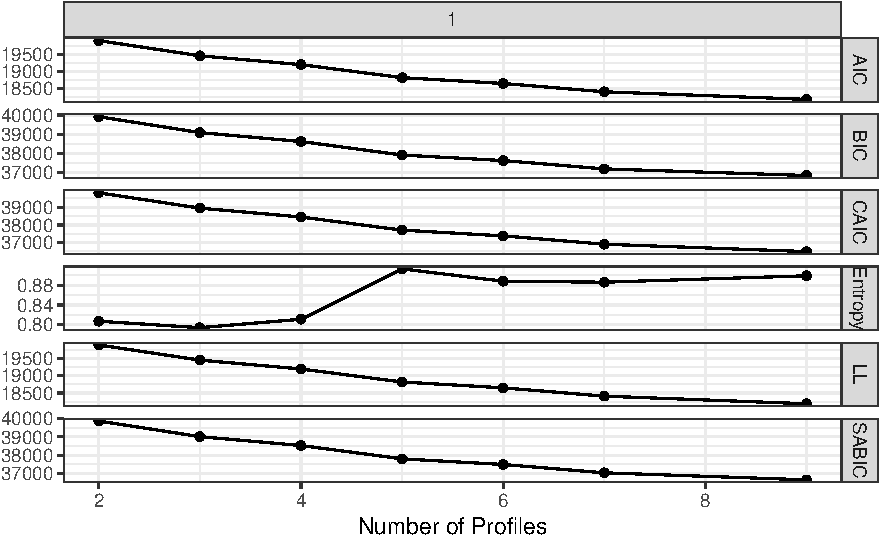
\includegraphics[width=0.5\linewidth]{rosenberg-dissertation_files/figure-latex/model1-1} 

}

\caption{Fit statistics for model 1 solutions}\label{fig:model1}
\end{figure}

\begin{figure}

{\centering 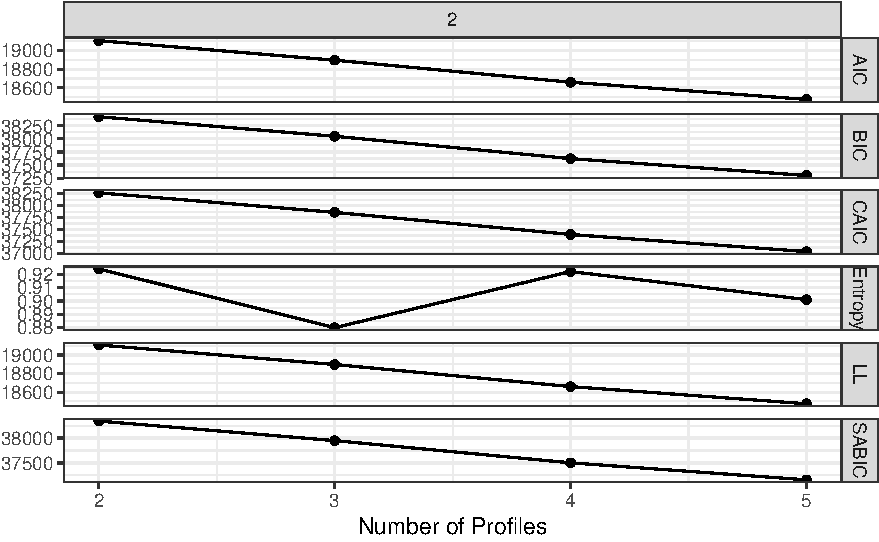
\includegraphics[width=0.4\linewidth]{rosenberg-dissertation_files/figure-latex/model2-1} 

}

\caption{Fit statistics for model 2 solutions}\label{fig:model2}
\end{figure}

Looking across the statistics presented, some general ideas about which
models are to be preferred emerge. Solutions are interpreted first for
each model individually and then across models with the goal of choosing
a smaller number of models to investigate in more detail.

For solutions associated with model 1, the decrease (indicating a
preferred model) in information criteria becomes smaller as the number
of profiles increases from 5 to 6 and 6 to 7. A solution associated with
8 profiles did not replicate the log-likelihood and the VLMR and LMR
suggest that the solution associated with 9 profiles did not fit better
than that with 8 profiles, suggesting that models with 7 or fewer
profiles be preferred. Considering these models, the entropy statistic
increases by a large amount between the solution associated with 4 and 5
profiles (and then decreases slightly between 5 and 6 and 6 and 7
profile solutions), suggesting (but not providing conclusive evidence)
that models 5, 6, or 7 may be preferred. The bootstrapped LRT suggests
that, until the log-likelihood is not replicated, every more complex
model be selected. Taking these pieces of evidence into conclusion, for
model 1, solutions associated with 4 through 7 may be considered in more
depth, with an emphasis on solutions associated with profiles with 5 and
6 profiles on the basis of the slowing of the decrease in the
information criteria associated with the solutions with greater profiles
than these, and the increase in the entropy from 4 to 5 (and 6) profile
solutions.

For solutions associated with model 2, only those associated with 2-5
profile solutions were associated with log-likelihoods that were
replicated. For these four models, the log-likelihood decreased in a
mostly consistent way, such that changes in the decrease are not as
evident as those associated with model 1. The entropy statistic
decreases from 2 to 3 profile solutions, increases from 3 to 4 profile
solutions, and then decreases slightly from 4 to 5 profile solutions,
providing some information that models associated with 4 profiles be
preferred to the others. All of the LRTs suggest that the more complex
model be selected, not providing clear information about which solutions
are to be preferred. On the basis of these pieces of evidence, models
with 3, 4, and 5 solutions may be considered in more depth. However,
there is a lack of consistent evidence favoring more or less complex
models.

\subsection{Comparison of model 1 and model 2 type
solutions}\label{comparison-of-model-1-and-model-2-type-solutions}

When looking across solutions, some overall patterns in terms of what
profiles emerge and some directions for which models are to be selected
for use in subsequent analysis can be identified. First, overall
patterns are discussed. In the table, which profiles emerge from which
solution is presented.

There is a wide range of profiles. Some appear very commonly,
particularly those (full and universally low) characterized by high or
low levels across all of the variables. Moderate profiles, both all
moderate (characterized by moderately high levels across all of the
variables) and moderately low (characterized by low levels across all of
the variables), also appeared commonly, particularly for the solutions
for model 1.

\begin{landscape}\begin{table}

\caption{\label{tab:compare-profiles-by-solution}Profile assignments by LPA solution (models and numbers of profiles)}
\centering
\resizebox{\linewidth}{!}{\begin{tabular}[t]{ccccccccccccc}
\toprule
\rotatebox{-60}{Number of Profiles} & \rotatebox{-60}{Full} & \rotatebox{-60}{All Moderate} & \rotatebox{-60}{Comptent but not Engaged or Challenged} & \rotatebox{-60}{Only Behavioral} & \rotatebox{-60}{Only Affective} & \rotatebox{-60}{Moderately Low} & \rotatebox{-60}{Engaged and Competent but not Challenged} & \rotatebox{-60}{Challenged but not Engaged or Comptent} & \rotatebox{-60}{Challenged} & \rotatebox{-60}{Highly Challenged} & \rotatebox{-60}{Universally Low} & \rotatebox{-60}{Comptent but not Challenged}\\
\midrule
\addlinespace[0.3em]
\multicolumn{13}{l}{\textbf{Model 1}}\\
\hspace{1em}3 & x & x &  &  &  &  &  &  &  &  & x & \\
\hspace{1em}4 & x & x &  &  &  &  &  &  &  &  & x & x\\
\hspace{1em}5 & x & x &  & x & x &  &  &  &  &  & x & \\
\hspace{1em}6 & x & x &  & x & x &  & x &  &  &  & x & \\
\hspace{1em}6 (alt) & x &  &  &  &  & x & x &  & x & x & x & \\
\hspace{1em}7 & x &  &  &  &  & x &  & x & x & x & x & x\\
\addlinespace[0.3em]
\multicolumn{13}{l}{\textbf{Model 2}}\\
\hspace{1em}7 (alt) & x &  &  &  &  & x &  & x & x & x & x & x\\
\hspace{1em}3 &  &  &  &  &  &  &  &  & x &  & x & x\\
\hspace{1em}4 &  &  &  &  &  &  & x &  & x & x & x & \\
5 & x & x &  &  &  &  &  &  &  & x & x & x\\
\bottomrule
\end{tabular}}
\end{table}
\end{landscape}

\subsection{Examination of specific candidate
models}\label{examination-of-specific-candidate-models}

Following from the in-depth exploration of the candidate solutions, in
this section, model solutions associated with specific model types and
the number of profiles are investigated. In particular, the model one
type, six profile, and model one type, seven profile solutions are
described. Descriptions of other candidate solutions is included in the
appendix. For all of the solutions, the raw data and the data that are
centered to have a mean equal to 0 and a standard deviation of 1 (thus,
the y-axis on each of the plots is labeled ``Z-score'').

\subsubsection{Model type: 1, Profiles:
6}\label{model-type-1-profiles-6}

This solution is characterized by:

\begin{itemize}
\tightlist
\item
  A \emph{full} profile, profile 6
\item
  An \emph{universally low} profile, profile 2
\item
  An \emph{all moderate} profile, profile 5--and, like, the model 1, six
  profile solution--with moderate levels of affective engagement
\item
  An \emph{only behaviorally engaged} profile, profile 1, with moderate
  levels of behavioral engagement, very low affective engagement, and
  moderately (low) levels of cognitive engagement and challenge and
  competence
\item
  An \emph{only affectively engaged} profile, profile 4, with moderate
  levels of affective engagement, low levels of behavioral engagement,
  and moderately (low) levels of cognitive engagement and challenge and
  competence
\item
  An \emph{engaged and competent but not challenged} profile, profile 3,
  characterized by high levels of each of the three dimensions of
  engagement and of competence, but with low levels of challenge
\end{itemize}

The number of observations associated with each of the profiles is
somewhat balanced, with the universally low profile with the largest
number of observations (\emph{n} = 667; the same number for this profile
as in the model 1, five profile solution), followed by the all moderate
profile (\emph{n} = 638). Each of the other four profiles were
associated with 300 to 400 observations. Unlike the model 1, four and
five profile solutions, which distinguished observations on
\emph{either} a condition of engagement (i.e., competence) or one of its
dimensions (i.e., cognitive, behavioral, and affective), this solution
was associated with profiles that distinguished observations on the
basis of both: There were profiles for only behaviorally and affectively
engaged and for engaged and competent but not challenged. This solution
is compelling because it appears to group students on the basis of
multiple of the indicators, and demonstrate viability on the basis of
the fit statistics (i.e., the tables and figure). The log-likelihood was
replicated two times, with the next lowest log-likelihood not being
replicated, followed by a log-likelihood that was replicated (at least)
seven times. This solution (associated with the log-likelihood that was
replicated {[}at least{]} seven times) could be investigated in further
detail, to see whether--and if so, how--it differs from the solution
interpreted here. This solution is a strong candidate for use in
subsequent analyses.

\begin{center}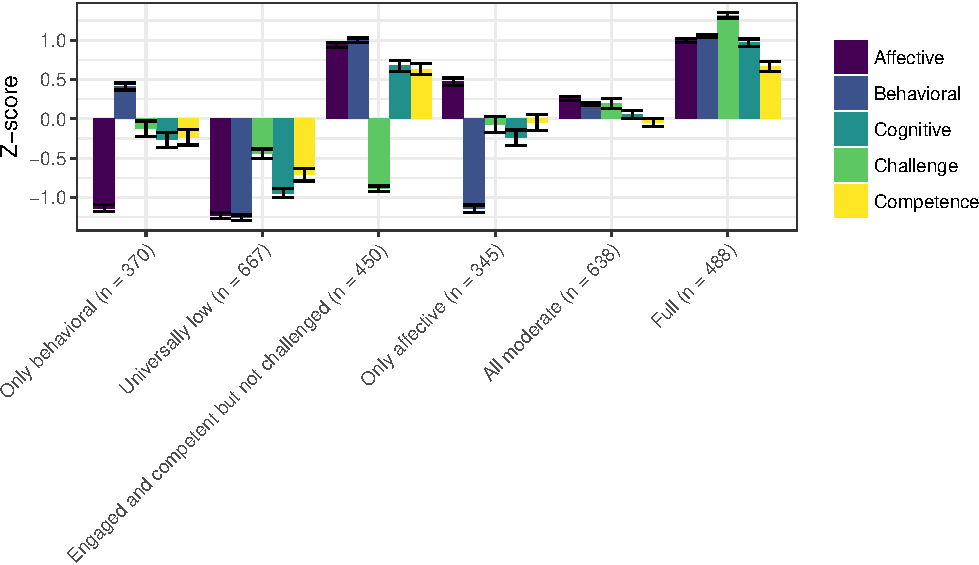
\includegraphics[width=0.95\linewidth]{rosenberg-dissertation_files/figure-latex/m1_6p-1} \end{center}

\begin{center}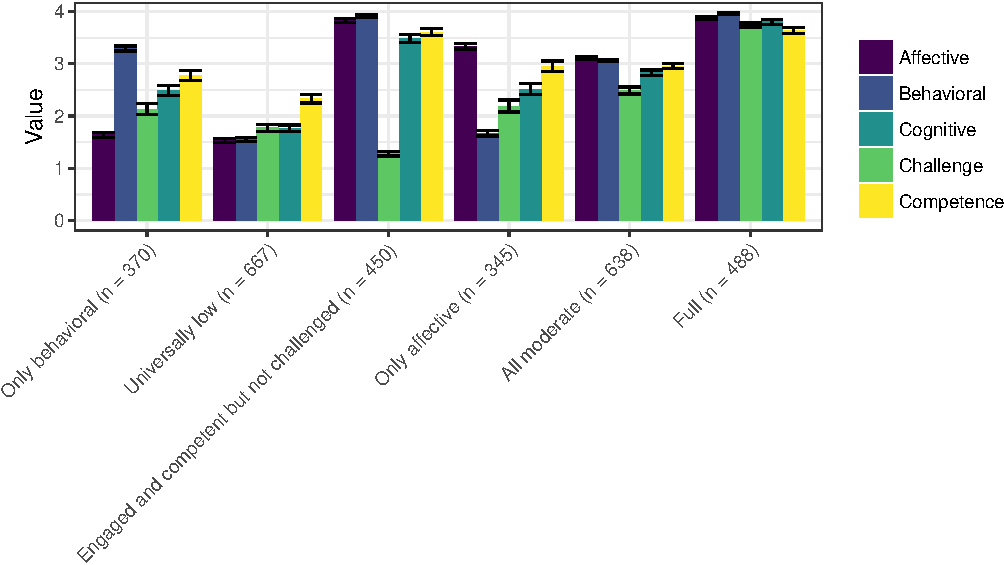
\includegraphics[width=0.95\linewidth]{rosenberg-dissertation_files/figure-latex/m1_6p-2} \end{center}

\begin{verbatim}
## Error: 'i.out' does not exist in current working directory ('/Users/joshuarosenberg/Google Drive/1_Research/dissertation/rosenberg-diss').
\end{verbatim}

\subsubsection{Model type: 1, Profiles:
7}\label{model-type-1-profiles-7}

This solution is characterized by:

\begin{itemize}
\tightlist
\item
  A \emph{full} profile, profile 7
\item
  A \emph{universally low} profile, profile 1
\item
  A \emph{competent but not engaged or challenged} profile, profile 2,
  characterized by high competence and moderate (low) or low levels of
  engagement and challenge
\item
  A \emph{moderately low} profile, profile 3, characterized by
  moderately low levels of all of the variables
\item
  A \emph{challenged} profile, profile 4, characterized by high
  challenge, moderate (high) levels of engagement, and moderate (low)
  levels of competence
\item
  A \emph{highly challenged} profile, profile 5, characterized by
  patterns similar to those of the challenged profile, but with higher
  challenge and with low levels of both engagement and challenge
\item
  A \emph{challenged but not engaged or competent} profile, profile 6,
  characterized by low levels of challenge, and high levels of
  engagement and competence
\end{itemize}

The number of observations associated with each of the profiles is not
very balanced, with few (\emph{n} = 181) observations associated with
the universally low profile and few (\emph{n} = 222) observations
associated with the highly challenged profile. The number of
observations associated with the other profiles ranged from 317 to 651.
Distinct from other solutions, none of the other five profiles were
found in the other model 1 solutions. Two pairs of the
profiles--challenged and highly challenged and universally low and
moderately low--exhibited similar patterns among the variables that were
distinguished by different mean levels. The log-likelihood was
replicated twice, with the next lowest log-likelihood being replicate
four times, possibly warranting further investigation. Taken together,
this solution raises questions about whether it may be too complex,
possibly suggesting preference for model 1 five and six profile
solutions.

\subsubsection{Looking across model 1 and model 2 type
solutions}\label{looking-across-model-1-and-model-2-type-solutions}

The model 1, six and seven profile solutions are compelling because both
show profiles that are distinguished by dimensions of engagement and its
conditions (challenge and competence). Note that for this model, only
the means and variances are estimated (and so no covariances are
estimated), and the variances are constrained to be the same across the
profiles. While this is a very restrictive model, it, along with the
model 3 type (which did not lead to solutions for any of the numbers of
profiles specified) also is a standard model for LPA, in that it meets
the assumption of local independence (of the variables that make up the
profiles--unlike for models in which covariances are estimated) typical
common to LPA (see Muthen \& Muthen, 2016). While some of the solutions
associated with the model 2 type did reach solutions, these demonstrated
less appealing properties in terms of their fit statistics as well as
their interpretability and with respect to concerns of parsimony. Thus,
while no covariances are estimated for the model 1 type solutions, there
is no requirement that these be specified; their benefit, when models
associated with them are preferred, is that they can provide better fit:
they can be used to better explain or predict the data in a sample, but
their inclusion also means that over-fitting the model to the data can
become a greater concern.

For each solution, alternate solutions associated with higher
log-likelihoods were explored. One advantage of the six profile solution
is that most of its profiles can also be identified in solutions with
fewer profiles. For the six profile solutions, this alternate solution
was very different, whereas for the seven profile solutions, this
alternate solution was highly similar. The model solutions exhibit a
less clear pattern in terms of which profiles appear when. All else
being equal, on the basis of parsimony, the model 1, six profile
solution may be preferred and is selected for use in subsequent
analyses.

As a type of sensitivity analysis focused on alternate model
specifications (different from the kind described earlier for
quantifying how robust an inference is to potential sources of bias or
confounding variables, e.g.~Frank, 2003), the model 1, seven profile
solution is also explored, but results for it are included in the
appendix. This model is less restrictive but does not meet the
assumption of independence; some scholars refer to it, as such, as a
general or Guassian mixture model solution, instead of an LPA solution
(Bauer, 2004). Because covariances are estimated, relationships between
the variables not captured in their mean levels estimated for each
profile are also estimated. This suggests that these models may be
modeling different relations between the variables than those associated
with model 1 and that they may fit the data better, but they are also
more complex and so should be interpreted with consideration these added
parameters.

\section{Research Question \#2: Relations Between Instructional Support
for Work With Data and the
PECs}\label{research-question-2-relations-between-instructional-support-for-work-with-data-and-the-pecs}

Broadly, this question is focused on how instructional support for work
with data, as coded from video-recordings of the programs, relates to
the PECs. For the primary results for this question, linear models that
account for the cross-classification of the moment and youth are used
and for the ``nesting'' of both within each of the nine programs are
used. For the outcome (\emph{y} variable), the probability of a response
belonging to the profile is used; thus, there are six models, for each
of the six profiles, for each specification of the predictor (\emph{x})
variables.

Null models showing the proportion of variance (via the intra-class
correlation) are interpreted. The more detailed results (in a table) are
presented in the appendix. These are followed by the interpretation of
findings related to a more variable-centered approach, namely,
correlations between individual aspects of work with data and the
composite and the profiles (and the variables that make them up) and
individual interest. Finally, results of mixed effects models with the
work with data variables added separate and then with the composite for
instructional support for work with data are interpreted and presented.

\subsection{Null models}\label{null-models}

The null models presented in the table provide insight into the levels
at which predictors may be able to explain the outcome. For all six
profiles, the ICCs were very small, from 0.00 to 0.023. This suggests
that very little variability can be explained simply by the program. For
the momentary level, the ICCs were also very small, ranging from 0.004
to 0.011. Finally, the youth-level ICCs ranged from .099 to .427.
Looking across these values, considering variability at the program,
momentary, and youth levels, most of the explained variability in the
responses is associated with youth; the program and momentary levels
were associated with very small values, suggesting that variables at
these levels have minimal variability that is able to be explained. In
turn, this suggests that these variables, including those for
instructional support for work with data, may not have strong effects in
terms of their relations with the PECs.

In terms of specific ICCs at the youth level, the value for the
youth-level ICC was highest for the \emph{full} profile, suggesting that
some youth have a strong tendency to be fully engaged (possibly due to
their initial interest or other individual characteristics and
differences). The other profile characterized by a consistent pattern
across all of the variables--the \emph{universally low} profile--had a
modest ICC, .265. Finally, a large amount of variability is associated
with the residual (variance that is not associated with the program,
momentary, or youth levels). This suggests that there is wide variation
in students' responses that may not be readily explained or predicted.

\subsection{Models with variables for aspects of instructional support
for work with data added
separately}\label{models-with-variables-for-aspects-of-instructional-support-for-work-with-data-added-separately}

When the predictor variables for work with data are added, some overall
patterns and specific findings can be identified. The only relations
with \emph{p}-values that were below the criterion for statistical
significance (.05) were for the relations between modeling data and the
\emph{full} profile (\emph{B} = 0.036 (0.016), \emph{p} = .016) and
between generating data and the full profile (\emph{B} = 0.029 (0.015),
\emph{p} = .024).

Adding these variables changed the (conditional upon the random effects)
r-squared values from, .002 to .018, very small changes suggesting that
the aspects of work with data do not strongly predict the PECs. This is
in-line with the correlations for these variables with those variables
that make up the profiles, and the ICC values at the momentary level.

The sensitivity analysis for the effect of generating data suggested
that 1.884\% of the inference would have to be due to bias to invalidate
the inference, suggesting that this effect is not very robust to
potential sources of bias, such as an omitted (in this analysis)
confounding (or control) variable. For the effect of modeling, 9.835\%
would need to be due to bias to invalidate the inference. This effect,
then, is less sensitive to possible sources of bias, but is still not
highly robust.

\begin{landscape}\begin{table}

\caption{\label{tab:rq2-1-tab-pres}Results of mixed effects models for instructional support for work with data as separate variables}
\centering
\resizebox{\linewidth}{!}{\begin{tabular}[t]{lllllllrrr}
\toprule
model & intercept & dm\_ask & dm\_obs & dm\_gen & dm\_mod & dm\_com & beep\_ID\_ICC & participant\_ID\_ICC & program\_ID\_ICC\\
\midrule
Only behavioral & 0.1 (0.014) (p < .001) & 0.013 (0.014) (p = 0.188) & 0.017 (0.014) (p = 0.122) & 0.009 (0.014) (p = 0.244) & -0.026 (0.015) (p = 0.957) & 0.025 (0.014) (p = 0.043) & 0.008 & 0.097 & 0.007\\
Universally low & 0.231 (0.029) (p < .001) & -0.008 (0.017) (p = 0.685) & 0.01 (0.017) (p = 0.277) & -0.017 (0.017) (p = 0.839) & 0.007 (0.018) (p = 0.356) & -0.006 (0.017) (p = 0.626) & 0.005 & 0.269 & 0.026\\
Engaged and competent but not challenged & 0.148 (0.016) (p < .001) & -0.012 (0.015) (p = 0.797) & 0.009 (0.015) (p = 0.267) & -0.016 (0.014) (p = 0.871) & 0.001 (0.015) (p = 0.487) & 0.008 (0.014) (p = 0.284) & 0.017 & 0.305 & 0.000\\
Only affective & 0.115 (0.011) (p < .001) & 0.005 (0.013) (p = 0.362) & -0.019 (0.013) (p = 0.919) & -0.015 (0.013) (p = 0.874) & -0.011 (0.014) (p = 0.787) & 0.012 (0.013) (p = 0.175) & 0.000 & 0.100 & 0.000\\
All moderate & 0.234 (0.02) (p < .001) & 0.016 (0.017) (p = 0.169) & 0.001 (0.016) (p = 0.477) & 0.015 (0.016) (p = 0.169) & -0.007 (0.017) (p = 0.651) & -0.009 (0.016) (p = 0.716) & 0.005 & 0.260 & 0.005\\
Full & 0.171 (0.025) (p < .001) & -0.017 (0.015) (p = 0.859) & -0.024 (0.015) (p = 0.943) & 0.029 (0.015) (p = 0.025) & 0.035 (0.016) (p = 0.016) & -0.03 (0.015) (p = 0.976) & 0.028 & 0.455 & 0.019\\
\bottomrule
\end{tabular}}
\end{table}
\end{landscape}

\subsection{Models with the composite
added}\label{models-with-the-composite-added}

For the composite of work with data, the composite predicted the profile
for \emph{only behavioral} (\emph{B} = 0.007 (0.004), \emph{p} = .021),
but not any of the other profiles. However, this coefficient is very
small in practical terms, and 12.261\% would need to be due to bias to
invalidate the inference. The change in r-squared values ranged from
.003 to .020, suggesting minimal potential relations among factors (such
as support for work with data as measured by the composite variable) at
the momentary level. When the composite was treated as a dichotomous
(instead of a continuous) variable, so that the variable takes a value
of one if any of the aspects of work with data are present, the results
are similar in terms of the magnitude of the effects and their
significance, as none of the relations are statistically significant
when the dichotomous variable is used.

\begin{landscape}\begin{table}

\caption{\label{tab:just-composite-red}Results of mixed effects models for the composite}
\centering
\resizebox{\linewidth}{!}{\begin{tabular}[t]{lllrrr}
\toprule
model & intercept & dm\_composite & beep\_ID\_ICC & participant\_ID\_ICC & program\_ID\_ICC\\
\midrule
Only behavioral & 0.104 (0.014) (p < .001) & 0.007 (0.004) (p = 0.021) & 0.008 & 0.097 & 0.008\\
Universally low & 0.229 (0.029) (p < .001) & -0.003 (0.004) (p = 0.784) & 0.004 & 0.269 & 0.026\\
Engaged and competent but not challenged & 0.148 (0.016) (p < .001) & -0.002 (0.004) (p = 0.754) & 0.016 & 0.305 & 0.000\\
Only affective & 0.117 (0.011) (p < .001) & -0.005 (0.003) (p = 0.912) & 0.000 & 0.100 & 0.000\\
All moderate & 0.234 (0.02) (p < .001) & 0.003 (0.004) (p = 0.212) & 0.005 & 0.259 & 0.005\\
Full & 0.168 (0.025) (p < .001) & -0.001 (0.004) (p = 0.599) & 0.030 & 0.452 & 0.021\\
\bottomrule
\end{tabular}}
\end{table}
\end{landscape}

\subsection{Summary of findings for research question
\#2}\label{summary-of-findings-for-research-question-2}

When looking across findings, we find few relations between
instructional support for work with data and the profiles, though there
were notable effects of modeling, though they were small effects (i.e.,
when students are doing this, they are around 3\% more likely to be
responding in a way associated with the \emph{full} profile). The
composite for work with data had a relation of around 0.01 with the
\emph{only behavioral} profile, suggesting that for each one-value
increase in the composite (which has a range from one to five), this
profile is around 1\% more likely. These findings are similar to those
obtained when the model 1 type, seven profile solution is used for the
outcome variables; see the appendix for more detail. Broadly, further
explanations and investigations of these effects --focusing on the
characteristics of instructional support for work with data in the
context of summer STEM programs and how this support is measured in
terms of codes from the video--are the focus on research question \#4
and are discussed in the next chapter. Moreover, these findings are
deepened in subsequent analyses for research questions \#3.

\section{Results for Research Question
\#3}\label{results-for-research-question-3}

Research question \#3 is focused on how the relationships of
instructional support for work with data differ on the basis of
pre-program interest and other youth characteristics. Like for the
previous two research questions, linear models that account for the
cross-classification of the moment and the youth--and their nesting
within the programs--are used. Findings from models with pre interest,
gender, and URM status are first presented. Then, models with these
variable and the individual aspects and composite of work with data are
added and then models with the interaction between these characteristics
and the composite.

\subsection{Models with pre interest, gender, and under-represented
minority (URM)
status}\label{models-with-pre-interest-gender-and-under-represented-minority-urm-status}

These results show that overall pre-interest is associated with the
\emph{engaged and competent but not challenged} profile (\emph{B} =
0.039 (0.021), p = .009). The effect of being a female has a relation of
0.059 (0.036, p = .054) upon the probability of a response being
associated with the \emph{universally low} profile; though this effect
did not meet the criteria for statistical significance, sensitivity
analysis to determine how much more robust the effect would need to be
to make an inference. For the effect of overall pre-interest upon the
\emph{engaged and competent but not challenged} profile, 17.879\% would
be needed to invalidate the inference, suggesting a moderately robust
effect. For the effect of gender upon the \emph{universally low}
profile, 16.996\% of the bias would need to be removed (or the effect
would need to be larger by this percentage) to sustain the inference.
The change in r-squared values ranged from .004 to .007, suggesting that
pre-interest and other individual characteristics - in addition to the
aspects of work with data - have minimal relations with the PECs. Thai
is more surprising than the similarly minimal relations observed for
work with data: as the null models indicate, there were large ICCs (a
large proportion of the variability in the outcome variables) at the
youth-level (as pre-interest, gender, and URM status are variables
associated with this level) This is discussed further in the next
chapter.

\begin{landscape}\begin{table}

\caption{\label{tab:reading-for-rq4}Results of mixed effects models with interest and other characteristics}
\centering
\resizebox{\linewidth}{!}{\begin{tabular}[t]{lllllrrr}
\toprule
model & intercept & overall\_pre\_interest & gender\_female & urm & beep\_ID\_ICC & participant\_ID\_ICC & program\_ID\_ICC\\
\midrule
Only behavioral & 0.131 (0.044) (p = 0.002) & -0.014 (0.011) (p = 0.89) & 0.018 (0.019) (p = 0.168) & 0.025 (0.026) (p = 0.168) & 0.006 & 0.091 & 0.012\\
Universally low & 0.33 (0.084) (p < .001) & -0.042 (0.021) (p = 0.974) & 0.059 (0.036) (p = 0.054) & -0.003 (0.051) (p = 0.525) & 0.005 & 0.276 & 0.012\\
Engaged and competent but not challenged & 0.017 (0.062) (p = 0.392) & 0.039 (0.016) (p = 0.009) & 0.026 (0.028) (p = 0.18) & -0.011 (0.04) (p = 0.613) & 0.014 & 0.306 & 0.000\\
Only affective & 0.075 (0.042) (p = 0.037) & 0.009 (0.011) (p = 0.214) & -0.022 (0.018) (p = 0.883) & 0.025 (0.025) (p = 0.159) & 0.011 & 0.094 & 0.005\\
All moderate & 0.374 (0.073) (p < .001) & -0.016 (0.019) (p = 0.806) & -0.037 (0.032) (p = 0.872) & -0.077 (0.046) (p = 0.952) & 0.005 & 0.258 & 0.006\\
Full & 0.084 (0.08) (p = 0.149) & 0.019 (0.02) (p = 0.17) & -0.036 (0.036) (p = 0.842) & 0.043 (0.051) (p = 0.2) & 0.030 & 0.452 & 0.001\\
\bottomrule
\end{tabular}}
\end{table}
\end{landscape}

\subsection{Models with pre interest, gender, and URM status and the
aspects of work with
data}\label{models-with-pre-interest-gender-and-urm-status-and-the-aspects-of-work-with-data}

These results show very similar patterns to those observed in the models
with pre-interest and the other individual characteristics and the
models with the aspects of work with data separate. Like in the models
with only pre-interest and the other individual characteristics,
pre-interest is related to the \emph{only behavioral} profile (\emph{B}
= 0.039 (0.016), p = .009). Being female is again related but not to a
level that it meets the criteria for statistical significance (\emph{B}
= 0.06 (0.037), p = .051). Generating data (\emph{B} = 0.027 (0.015), p
= .033) and modeling data (\emph{B} = 0.034 (0.017), p = .020) were both
related to the \emph{full} profile to a similar extent and with similar
robustness as found in the separate models. Compared to the null models,
the r-squared values changed from .001 to .029, suggesting small
improvements from the additions of the individual characteristics and
the codes for the aspects of work with data.

\begin{landscape}\begin{table}

\caption{\label{tab:pre-int-ind-present}Results of mixed effects models with interest and other characteristics and the aspects of work with data}
\centering
\resizebox{\linewidth}{!}{\begin{tabular}[t]{llllllllllrrr}
\toprule
model & intercept & dm\_ask & dm\_obs & dm\_gen & dm\_mod & dm\_com & overall\_pre\_interest & gender\_female & urm & beep\_ID\_ICC & participant\_ID\_ICC & program\_ID\_ICC\\
\midrule
Only behavioral & 0.107 (0.045) (p = 0.01) & 0.015 (0.015) (p = 0.158) & 0.013 (0.015) (p = 0.191) & 0.014 (0.014) (p = 0.17) & -0.023 (0.016) (p = 0.929) & 0.018 (0.015) (p = 0.115) & -0.013 (0.012) (p = 0.873) & 0.019 (0.019) (p = 0.159) & 0.031 (0.026) (p = 0.122) & 0.008 & 0.095 & 0.010\\
Universally low & 0.356 (0.086) (p < .001) & -0.015 (0.018) (p = 0.789) & 0.003 (0.018) (p = 0.427) & -0.014 (0.017) (p = 0.789) & 0.004 (0.019) (p = 0.407) & 0.002 (0.018) (p = 0.461) & -0.047 (0.022) (p = 0.982) & 0.06 (0.037) (p = 0.051) & -0.01 (0.052) (p = 0.575) & 0.005 & 0.276 & 0.015\\
Engaged and competent but not challenged & 0.022 (0.063) (p = 0.362) & -0.011 (0.015) (p = 0.763) & 0.009 (0.015) (p = 0.266) & -0.014 (0.014) (p = 0.833) & 0 (0.015) (p = 0.504) & 0.004 (0.015) (p = 0.404) & 0.039 (0.016) (p = 0.009) & 0.025 (0.028) (p = 0.188) & -0.012 (0.04) (p = 0.614) & 0.015 & 0.304 & 0.000\\
Only affective & 0.09 (0.04) (p = 0.015) & 0.004 (0.014) (p = 0.397) & -0.017 (0.014) (p = 0.886) & -0.02 (0.013) (p = 0.938) & -0.012 (0.015) (p = 0.8) & 0.016 (0.014) (p = 0.124) & 0.007 (0.01) (p = 0.264) & -0.02 (0.018) (p = 0.867) & 0.018 (0.025) (p = 0.234) & 0.000 & 0.095 & 0.001\\
All moderate & 0.354 (0.075) (p < .001) & 0.023 (0.017) (p = 0.09) & 0.007 (0.017) (p = 0.342) & 0.012 (0.016) (p = 0.233) & -0.004 (0.018) (p = 0.593) & -0.011 (0.017) (p = 0.747) & -0.012 (0.019) (p = 0.743) & -0.038 (0.033) (p = 0.875) & -0.076 (0.046) (p = 0.95) & 0.005 & 0.256 & 0.007\\
Full & 0.094 (0.083) (p = 0.132) & -0.019 (0.016) (p = 0.887) & -0.025 (0.016) (p = 0.94) & 0.027 (0.015) (p = 0.033) & 0.034 (0.017) (p = 0.02) & -0.027 (0.016) (p = 0.956) & 0.018 (0.021) (p = 0.195) & -0.035 (0.037) (p = 0.827) & 0.043 (0.053) (p = 0.207) & 0.027 & 0.476 & 0.002\\
\bottomrule
\end{tabular}}
\end{table}
\end{landscape}

\subsection{Models with pre-interest, gender, and URM status and work
with data
composite}\label{models-with-pre-interest-gender-and-urm-status-and-work-with-data-composite}

Like for the individual aspects, these models with the composite for
work with data instead of the individual aspects. These results show
very similar patterns to those observed in the models with pre-interest
and the other individual characteristics and the models with the aspects
of work with data separate. Like in the models with only pre-interest
and the other individual characteristics alone (and like in the model
with the individual aspects), pre-interest is related to the \emph{only
behavioral} profile (\emph{B} = 0.039 (0.016), p = .009). Being female
is again related but not to a level that it meets the criteria for
statistical significance (\emph{B} = 0.06 (0.037), p = .052). The
composite was significantly related to the \emph{only behavioral}
profile (\emph{B} = 0.007 (0.004), p = .027) to a similar extent and
with similar robustness as found in the separate model. Compared to the
null models, the r-squared values changed from .008 to .026, once again
suggesting small improvements from the additions of the individual
characteristics and the composite for the aspects of work with data.

\begin{landscape}\begin{table}

\caption{\label{tab:pre-int-int-present}Results of mixed effects models with interest and other characteristics and the composite work with data}
\centering
\resizebox{\linewidth}{!}{\begin{tabular}[t]{llllllrrr}
\toprule
model & intercept & dm\_composite & overall\_pre\_interest & gender\_female & urm & beep\_ID\_ICC & participant\_ID\_ICC & program\_ID\_ICC\\
\midrule
Only behavioral & 0.111 (0.045) (p = 0.008) & 0.007 (0.004) (p = 0.027) & -0.013 (0.012) (p = 0.874) & 0.02 (0.019) (p = 0.149) & 0.03 (0.026) (p = 0.126) & 0.007 & 0.095 & 0.010\\
Universally low & 0.355 (0.086) (p < .001) & -0.004 (0.005) (p = 0.824) & -0.047 (0.022) (p = 0.983) & 0.06 (0.037) (p = 0.052) & -0.01 (0.052) (p = 0.573) & 0.003 & 0.277 & 0.015\\
Engaged and competent but not challenged & 0.022 (0.063) (p = 0.364) & -0.003 (0.004) (p = 0.783) & 0.039 (0.016) (p = 0.009) & 0.025 (0.028) (p = 0.19) & -0.011 (0.04) (p = 0.608) & 0.014 & 0.305 & 0.000\\
Only affective & 0.094 (0.041) (p = 0.012) & -0.005 (0.003) (p = 0.93) & 0.006 (0.01) (p = 0.293) & -0.02 (0.018) (p = 0.863) & 0.019 (0.025) (p = 0.226) & 0.000 & 0.095 & 0.002\\
All moderate & 0.354 (0.075) (p < .001) & 0.005 (0.004) (p = 0.111) & -0.012 (0.019) (p = 0.743) & -0.037 (0.033) (p = 0.872) & -0.076 (0.046) (p = 0.95) & 0.005 & 0.256 & 0.008\\
Full & 0.089 (0.083) (p = 0.144) & -0.001 (0.004) (p = 0.62) & 0.019 (0.021) (p = 0.184) & -0.037 (0.037) (p = 0.84) & 0.044 (0.053) (p = 0.205) & 0.029 & 0.473 & 0.002\\
\bottomrule
\end{tabular}}
\end{table}
\end{landscape}

\subsection{Models with interactions between pre interest, gender, and
URM status and work with data
composite}\label{models-with-interactions-between-pre-interest-gender-and-urm-status-and-work-with-data-composite}

These results show similar patterns to the earlier models.Like in the
models with only pre-interest and the other individual characteristics
alone (and like in the model with the individual aspects), pre-interest
is related to the \emph{only behavioral} profile (\emph{B} = 0.033
(0.018), p = .033). Being female is again related but not to a level
that it meets the criteria for statistical significance (\emph{B} =
0.064 (0.041), p = .059). With the interactions added, the composite was
no significantly related to the \emph{only behavioral} profile (\emph{B}
= 0.016 (0.016), p = .156) to a similar extent and with similar
robustness as found in the separate model. One interaction, between
pre-interest and being female, had a significant effect upon the profile
for \emph{full} engagement (\emph{B} = 0.012 (0.006), p = .026).
However, only 1.953\% of the effect would need to be due to bias to
invalidate the inference. The r-squared values, relative to the models
with only random effects (the null models), increased from .003 to .028,
again suggesting small effects of the predictors upon the PECs.

\begin{landscape}\begin{table}

\caption{\label{tab:pre-int-comp}Results of mixed effects models with the interactions between interest and other characactistics and the composite for work with data}
\centering
\resizebox{\linewidth}{!}{\begin{tabular}[t]{lllllllllrrr}
\toprule
model & intercept & dm\_composite & overall\_pre\_interest & gender\_female & urm & overall\_pre\_interest:dm\_composite & dm\_composite:gender\_female & dm\_composite:urm & beep\_ID\_ICC & participant\_ID\_ICC & program\_ID\_ICC\\
\midrule
Only behavioral & 0.095 (0.054) (p = 0.041) & 0.016 (0.016) (p = 0.156) & -0.01 (0.014) (p = 0.764) & 0.018 (0.024) (p = 0.219) & 0.04 (0.033) (p = 0.114) & -0.002 (0.004) (p = 0.655) & 0.001 (0.007) (p = 0.458) & -0.005 (0.01) (p = 0.691) & 0.008 & 0.095 & 0.010\\
Universally low & 0.373 (0.093) (p < .001) & -0.013 (0.019) (p = 0.756) & -0.051 (0.024) (p = 0.982) & 0.064 (0.041) (p = 0.059) & -0.018 (0.057) (p = 0.623) & 0.002 (0.005) (p = 0.335) & -0.002 (0.009) (p = 0.575) & 0.004 (0.012) (p = 0.361) & 0.004 & 0.276 & 0.015\\
Engaged and competent but not challenged & 0.021 (0.068) (p = 0.378) & -0.002 (0.015) (p = 0.559) & 0.033 (0.018) (p = 0.033) & 0.041 (0.031) (p = 0.093) & 0.002 (0.044) (p = 0.479) & 0.003 (0.004) (p = 0.22) & -0.008 (0.007) (p = 0.885) & -0.006 (0.009) (p = 0.753) & 0.015 & 0.303 & 0.000\\
Only affective & 0.078 (0.05) (p = 0.059) & 0.003 (0.015) (p = 0.424) & 0.018 (0.013) (p = 0.078) & -0.02 (0.023) (p = 0.813) & -0.008 (0.031) (p = 0.604) & -0.006 (0.004) (p = 0.946) & -0.001 (0.007) (p = 0.539) & 0.013 (0.009) (p = 0.079) & 0.000 & 0.096 & 0.002\\
All moderate & 0.337 (0.082) (p < .001) & 0.013 (0.018) (p = 0.236) & -0.013 (0.021) (p = 0.731) & -0.043 (0.036) (p = 0.882) & -0.052 (0.051) (p = 0.842) & 0 (0.005) (p = 0.476) & 0.003 (0.008) (p = 0.344) & -0.012 (0.011) (p = 0.864) & 0.005 & 0.256 & 0.008\\
Full & 0.119 (0.087) (p = 0.087) & -0.017 (0.014) (p = 0.886) & 0.016 (0.022) (p = 0.232) & -0.061 (0.039) (p = 0.94) & 0.032 (0.056) (p = 0.283) & 0.002 (0.004) (p = 0.337) & 0.012 (0.006) (p = 0.026) & 0.005 (0.009) (p = 0.264) & 0.029 & 0.476 & 0.001\\
\bottomrule
\end{tabular}}
\end{table}
\end{landscape}

\subsection{Summary of findings for research question
\#3}\label{summary-of-findings-for-research-question-3}

When looking across findings, we find minimal relations between
pre-interest and other individual characteristics. In particular, we
found that pre-interest was related to the \emph{engaged and comptent
but not challenged} profile to a modest extent. Being female did not
demonstrate statistically significant relations with the
\emph{univerally low} profile, though some moderately-sized effects that
were nearly statistically significant were observed and interpreted in
terms of how much bias would need to be reduced (or how much the larger
the effect would need to be) in order for this relation to be
statistically significant. These results, like those for research
question \#2, are similar to those obtained when the model 1 type, seven
profile solution is used for the outcome variables. There were few
interactive effects observed; the magnitude of the effect of the
composite and gender interaction was small (as were the changes in the
r-squared value as a consequence of adding this interaction), and the
effect appears to not be highly robust to potential sources of bias.
Like for research question \#2, reasons for why this may be are explored
in the next chapter. The effect of the activity appears robust, as in
research question \#3

\section{Results for Research Question
\#4}\label{results-for-research-question-4}

To code the data, three research assistants were trained for
approximately eight hours over four meetings. Then, each research
assistant coded all of the segments associated with one of the videos.
After the coding was complete, the three research assistants and I met
to discuss how well the coding frame and potential sources of
disagreement. Then, two coders coded every segment that was coded for at
least one of the aspects of instructional support for work with data.
This coding took around 75 hours of coding by the research assistants.
After each program, the coders met to discuss potential issues that
emerged throughout the coding, and to clarify how they applied the
coding frame. As this was open-ended coding with the aim to provide
greater detail and context for the findings associated with research
questions \#2 and \#3, establishing reliability among the coders was not
carried out. The coders sought to document a) the characteristics of
instructional support for work with data and b) other aspects of the
instructional context that impacts student work with data.

Note that while the first of the two aspects focuses on the support
provided by the instructor, the second aspect focuses on how students
engage in work with data in ways that on occasion diverge (in ways
productive and not productive in terms of student work with data) from
what would be expected on the basis of the instructional support. This
coding resulted in around three to four sentence notes associated with
each segment from each of two raters. Then, I reviewed these notes with
the aim to identify themes based on enriching and better understanding
the findings for research questions \#2-\#4 and, beyond these findings,
to better understand the nature of work with data in summer STEM
programs.

\subsection{Affordances and constraints of summer STEM programs for work
with
data}\label{affordances-and-constraints-of-summer-stem-programs-for-work-with-data}

Summer STEM program have affordances and constraints work with data.
Thus, different from the previous theme that was focused on a
study-related issue, this theme concerns differences in the nature of
the instruction and learning opportunities that learners experienced as
part of their time in the summer STME programs.

\subsubsection{Affordances}\label{affordances}

Affordances included the community setting and the relevance of the
program to youth's lives.

For example, in the \emph{Marine Investigators}, youth participated in
activities designed to help them understand water quality in their
ecosystem. Youth collected trash from sites around their community (in
different ``districts'') and then brought the trash and recyclable
plastic back to the classroom. Then, the youth activity leaders asked
students to figure out how much plastic enters local waterways. As a
part of this activity, youth activity leaders asked students not only to
determine the quantity of trash that entered the waterways, but asked
students about \emph{why} they used math in particular ways (i.e.,
adding the quantity of trash collected and then extrapolating from this
quantity to the amount from across the entire city over the course of
the year). This appeared to be a powerful activity, one that was coded
as involving all five aspects of work with data according to the
measures for instructional support for work with data; this type of
activity seemed to suggest that instructional support for work with data
may impact youth's engagement.

Another affordance concerned the relevance of the program to youth's
lives. For example, in the \emph{Building Mania} program, youth are
involved in engineering design (i.e., identifying a problem and
designing a solution), particularly around the use of simple machines.
In a day in the classroom setting, youth are creating, testing, and
revising catapults. In the next day, youth visit an area University, and
are led in a discussion by a physicist who works with particle
colliders. In this example, the expertise of the physicist, who
explicitly mentions the benefits of engaging in the engineering design
process and the importance of combining engineering to addressing
problems (such as mitigating the damage of earthquakes), seems to be
highly relevant to what youth are doing in their class. In these two
days of class, youth are engaged in different aspects of work with data
as indicated by the codes for instructional support for work with data
(collecting data on the efficacy of their designs in the classroom day,
and asking questions in the subsequent day, particularly); these seem to
suggest, like the example of work work with data from the \emph{Marine
Investigators} program, affordances of work with data for summer STEM
programs.

\subsubsection{Constraints}\label{constraints}

Constraints included the challenge of linking activities as a part of a
complete cycle of investigation and an emphasis on different aspects of
work with data as part of programming.

Youth activity leaders faced challenges linking activities as part of a
complete cycle of investigation. For example, in the \emph{Ecosphere}
program, youth collected water samples in the field. They then brought
these samples to the classroom and tested the water, involving students
in both collecting and, to a degree, generating data (by noting the pH
levels of the water). However, later in the day, youth created a
small-scale model (with inclined trays of dirt, rocks, and plants) of an
ecosystem, in which they added food coloring to determine the impacts of
chemicals and acid rain. Youth then interpreted and discussed these
findings, but did not connect the discussion to the water samples youth
collected and tested earlier. This activity presented an opportunity for
deeper engagement, in which youth could interpret and communicate
findings related to the state of the water in their ecosystem, but,
instead, it was potentially limiting in terms of youth's engagement in
work with data.

A theme related to the challenge of linking activities concerned what
the programs focused on. For example, the mathematics-focused programs,
such as the \emph{Adventures in Mathematics} program, the youth activity
leaders recognizing that youth had difficulty solving equations, used
duct tape and a ``hippity hoppity'', building on an earlier activity in
which youth considered what constituted a rate, on how many ``hops'' it
would take someone to move from one end of the line of duct tape to the
other; the youth activity leader than asked youth to consider how far
they could move in one hop and to consider how they could find out many
hops it would take, using a mathematical equation. In this activity,
youth were supported to approach mathematics problem-solving in creative
ways. However, apart from data modeling, other aspects of work with data
were rarely present, and most of the data that youth worked with was
provided by the teacher or considered in the abstract. Programs focused
on science or engineering, similarly, emphasized other aspects of work
with data: The science-focused programs (\emph{Island Explorers},
\emph{The Ecosphere}, and \emph{Marine Investigators}) all emphasized
collecting and generating data, but data, particularly the data
collected or generated, was rarely modeled or interpreted. In the
engineering-focused programs (\emph{Uptown Architecture}, \emph{Crazy
Machines}, and \emph{Dorchester House}, youth often collected data that
resulted from their engineering designs, and communicated and
interpreted their findings, but, did not generate data, and,
accordingly, (and like the science-focused programs) did not model data
as a regular part of their activities. This finding suggests that while
work with data may have been common overall, different aspects of
instructional support for work with data were emphasized to different
degrees based on the focus of the program.

\subsection{How instructional support for work with data was
measured}\label{how-instructional-support-for-work-with-data-was-measured}

This theme concerned how instructional support was measured and how this
impacted the findings presented in research questions \#2 and \#3. As an
example, in a video associated with a mathematics-focused activity in
the Comunidad de Aprendizaje program, a youth activity leader is
discussing with youth opportunities for them to market products that
they developed to sell in their communities and highlighting the expense
of creating the product, its sale price, and its potential process. In
this example, observing data is coded, but this aspect of instructional
support for work with data does not appear to be present. Considering
the STEM-PQA code on which the code for making observations is based,
this difference is possibly due to a distinction in what both codes are
focused on. The STEM-PQA code is for \emph{classifying or abstracting},
and its operationalization emphasizes staff supporting youth in linking
concrete examples to principles, categories, or formulas. The conceptual
definition of \emph{making observations}, though, emphasizes watching
and noticing what is happening with respect to the phenomena being
investigated. In this case, the application of the STEM-PQA code was
sensible, as the youth activity leader was connecting the products youth
created to mathematical ideas (formulas) for how much they could expect
to earn from the sale of their products; in terms of work with data,
however, youth were not observing or noticing phenomena. This suggests
that differences in how work with data was conceptualized and
operationalized may lead, in some cases, to codes that do not reflect
work with data accurately, and can lead to some findings that seem
unexpected given what we know about the potential for work with data to
be engaging to youth.

\subsection{Summary of Findings for Research Question
\#4}\label{summary-of-findings-for-research-question-4}

These findings focused on the affordances and constrained of work with
data in summer STEM programs and how instructional support for work with
data was measured. Broadly, the qualitative analysis suggested possible
explanations for the findings for research questions \#2 and \#3. For
these questions, little variability was found to exist at the momentary
level, and the predictors at the momentary level (instructional support
for work with data) and at the youth level (pre-interest, gender, and
URM status) demonstrated modest relations with the profiles. These
relations can be due to a variety of reasons, particularly 1) how the
variables for the PECs and how instructional support for work with data
is measured, and 2) how suitable of summer STEM programs for work with
data. Accordingly, this analysis resulted in findings organized around
the following two themes. The first theme concerned \emph{affordances
and constraints of summer STEM programs for work with data}. The second
concerned \emph{howinstructional support for work with data was
measured}. Both are described in the remainder of this section. Another
possible explanation related to whether PECs and the variables that make
them up are appropriate outcomes, and how the PECS are measured, is an
important question, but one that cannot readily be assessed from the
video data that was analyzed; however, this topic is explored in the
next chapter.

\chapter{Discussion}\label{discussion}

\subsection{Key Findings}\label{key-findings}

\paragraph{The nature of engagement in summer STEM
programs}\label{the-nature-of-engagement-in-summer-stem-programs}

We can identify profiles of engagement \ldots{}

\paragraph{What explains PECs}\label{what-explains-pecs}

Engagement varies from moment-to-moment \ldots{}

\paragraph{Summer STEM programs as a context for work with
data}\label{summer-stem-programs-as-a-context-for-work-with-data}

\subsection{Limitations of the Study}\label{limitations-of-the-study}

\paragraph{Measurement issues}\label{measurement-issues}

How instructional support for work with data was measured seems to have
been an issue, given the qualitative coding \ldots{}

\paragraph{Context issues}\label{context-issues}

These programs were not designed to support work with data \ldots{}

\subsection{Recommendations for Future
Research}\label{recommendations-for-future-research}

\paragraph{Explore work with data in settings designed to support
it}\label{explore-work-with-data-in-settings-designed-to-support-it}

There are increasingly ``data camps'' \ldots{}

\paragraph{Measure student work with data as well as instructional
support for work with
data}\label{measure-student-work-with-data-as-well-as-instructional-support-for-work-with-data}

Measuring what students do in addition to what teachers do is important
\ldots{}

\paragraph{Explore changes in longer-term
outcomes}\label{explore-changes-in-longer-term-outcomes}

Changes in longer-term outcomes, such as future plans and goals, are an
important goal for summer STEM educators and other stakeholders in such
programs \ldots{}

\subsection{Implications for Practice}\label{implications-for-practice}

\paragraph{Engage students in complete cycles of
investigation}\label{engage-students-in-complete-cycles-of-investigation}

\paragraph{Support engagement in specific
moments}\label{support-engagement-in-specific-moments}

Viewing engagement in work with data in terms of engagement can help us
to build the knowledge base around key data analytic practices for
learners. In STEM settings, being engaged predicts key learning-related
outcomes (Sinatra et al., 2015). As a consequence, what learners are
thinking, feeling, and doing while engaged in work with data, and how
challenged or good at data doing any or all of the aspects of work with
data they perceive themselves to be, may important predictors of key
outcomes and learners' preparation for future learning (Bransford \&
Schwartz, 1999), especially for learning in data-rich areas of studies
and occupations, such as data science. Engaging in work with data may
also prepare learners to think of, understand, and take action based on
data in their day-to-day lives.

\chapter{References}\label{references}

\setlength{\parindent}{-0.5in} \setlength{\leftskip}{0.5in}

Akiva, T. (2005). Turning training into results: The new youth program
quality assessment. High/Scope Resource, 24(2), 21-24.\\
Bergman, L. R., \& Magnusson, D. (1997). A person-oriented approach in
research on developmental psychopathology. Development and
psychopathology, 9(2), 291-319.\\
Bergman, L. R., Magnusson, D., \& El Khouri, B. M. (2003). Studying
individual development in an interindividual context: A person-oriented
approach. Psychology Press.\\
Berland, L. K., Schwarz, C. V., Krist, C., Kenyon, L., Lo, A. S., \&
Reiser, B. J. (2016). Epistemologies in practice: Making scientific
practices meaningful for students. Journal of Research in Science
Teaching, 53(7), 1082-1112.\\
Bielik, T., \& Yarden, A. (2016). Promoting the asking of research
questions in a high-school biotechnology inquiry-oriented program.
International Journal of STEM Education, 3(1), 15.\\
Breckenridge, J. N. (2000). Validating cluster analysis: Consistent
replication and symmetry. Multivariate Behavioral Research, 35(2),
261-285.\\
Bystydzienski, J. M., Eisenhart, M., \& Bruning, M. (2015). High school
is not too late: Developing girls' interest and engagement in
engineering careers. Career Development Quarterly, 63(1), 88--95.
\url{http://doi.org/10.1002/j.2161-0045.2015.00097.x} Cohen, J. (1992).
A power primer. Psychological Bulletin, 112(1), 155.\\
National Governors Association Center for Best Practices, Council of
Chief State School Officers. (2010). Common Core State Standards for
Mathematics. Washington, DC: National Governors Association Center for
Best Practices and the Council of Chief State School Officers.\\
Corpus, J. H., \& Wormington, S. V. (2014). Profiles of intrinsic and
extrinsic motivations in elementary school: A longitudinal analysis. The
Journal of Experimental Education, 82(4), 480-501.\\
Csikszentmihalyi, M. (1990). Flow: The psychology of optimal
performance. Cambridge, England: Cambridge University Press.\\
Csikszentmihalyi, M. (1997). Finding flow: The psychology of engagement
with everyday life. New York, NY: Basic Books.\\
Creswell, J. W., Plano Clark, V. L., Gutmann, M. L., \& Hanson, W. E.
(2003). Advanced mixed methods research designs. In A. Tashakkori \& C.
Teddlie (Eds.), Handbook of mixed methods in social and behavioral
research (pp.~209--240). Thousand Oaks, CA: Sage.\\
English, L. D. (2012). Data modelling with first-grade students.
Educational Studies in Mathematics, 81(1), 15-30.\\
Finzer, W. (2013). The data science education dilemma. Technology
Innovations in Statistics Education, 7(2), p.~1-9.\\
Forum for Youth Investment. (2012). Youth Program Quality Assessment.
Washington, DC: The Forum for Youth Investment Franklin, C., Kader, G.,
Mewborn, D., Moreno, J., Peck, R., Perry, M., \& Scheaffer, R. (2007).
Guidelines for assessment and instruction in statistics education
(GAISE) report. Alexandria, VA: American Statistical Association.\\
Fredricks, J. A., \& McColskey, W. (2012). The measurement of student
engagement: A comparative analysis of various methods and student
self-report instruments. In S. L. Christenson, A. L. Reschly, \& C.
Wylie (Eds.), The handbook of research on student engagement
(pp.~763--782). New York: Springer Science.
\url{https://doi.org/10.1007/978-1-4614-2018-7_37}\\
Fredricks, J. A., Blumenfeld, P. C., \& Paris, A. H. (2004). School
engagement: Potential of the concept, state of the evidence. Review of
Educational Research, 74(1), 59-109.\\
Fredricks, J. A., Filsecker, M., \& Lawson, M. A. (2016). Student
engagement, context, and adjustment: Addressing definitional,
measurement, and methodological issues. Learning \& Instruction, 43,
1-4.\\
Gelman, S. A., \& Markman, E. M. (1987). Young children's inductions
from natural kinds: The role of categories and appearances. Child
Development, 58(6), 1532-1541.\\
Gopnik, A., \& Sobel, D. M. (2000). Detecting blickets: How young
children use information about novel causal powers in categorization and
induction. Child Development, 71(5), 1205-1222.\\
Gopnik, A., Sobel, D. M., Schulz, L. E., \& Glymour, C. (2001). Causal
learning mechanisms in very young children: two-, three-, and
four-year-olds infer causal relations from patterns of variation and
covariation. Developmental Psychology, 37(5), 620.\\
Greene, B. A. (2015). Measuring cognitive engagement with self-report
scales: Reflections from over 20 years of research. Educational
Psychologist, 50(1), 14-30.\\
Greene, K. M., Lee, B., Constance, N., \& Hynes, K. (2013). Examining
youth and program predictors of engagement in out-of-school time
programs. Journal of Youth and Adolescence, 42(10), 1557-1572.\\
Hancock, C., Kaput, J. J., \& Goldsmith, L. T. (1992). Authentic inquiry
with data: Critical barriers to classroom implementation. Educational
Psychologist, 27(3), 337-364.\\
Harring, J. R., \& Hodis, F. A. (2016). Mixture modeling: Applications
in educational psychology. Educational Psychologist, 51(3-4), 354-367.\\
Hasson, E., \& Yarden, A. (2012). Separating the research question from
the laboratory techniques: Advancing high‐school biology teachers'
ability to ask research questions. Journal of Research in Science
Teaching, 49(10), 1296-1320.\\
Hayenga, A. O., \& Corpus, J. H. (2010). Profiles of intrinsic and
extrinsic motivations: A person-centered approach to motivation and
achievement in middle school. Motivation and Emotion, 34(4), 371-383.\\
Hektner, J. M., Schmidt, J. A., \& Csikszentmihalyi, M. (2007).
Experience sampling method: Measuring the quality of everyday life.
Sage.\\
Jahnukainen, M. (2010). Extreme cases. Encyclopedia of Case Study
Research. Thousand Oaks, CA: Sage. Konold, C., \& Pollatsek, A. (2002).
Data analysis as the search for signals in noisy processes. Journal for
Research in Mathematics Education, 33(4), 259-289.\\
Lauer, P. A., Akiba, M., Wilkerson, S. B., Apthorp, H. S., Snow, D., \&
Martin-Glenn, M. L. (2006). Out-of-school-time programs: A meta-analysis
of effects for at-risk students. Review of educational research, 76(2),
275-313.\\
Lee, H. S., Angotti, R. L., \& Tarr, J. E. (2010). Making comparisons
between observed data and expected outcomes: students' informal
hypothesis testing with probability simulation tools. Statistics
Education Research Journal, 9(1), 68-96.\\
Lee, H., \& Hollebrands, K. (2008). Preparing to teach mathematics with
technology: An integrated approach to developing technological
pedagogical content knowledge. Contemporary Issues in Technology and
Teacher Education, 8(4), 326-341.\\
Lehrer, R., \& Romberg, T. (1996). Exploring children's data modeling.
Cognition and Instruction, 14(1), 69-108.\\
Lehrer, R., \& Schauble, L. (2004). Modeling natural variation through
distribution. American Educational Research Journal, 41(3), 635-679.\\
Lehrer, R. \& Schauble, L. (2015). Developing scientific thinking. In L.
S. Liben \& U. Müller (Eds.), Cognitive processes. Handbook of child
psychology and developmental science (Vol. 2, 7th ed., pp.~671-174).
Hoboken, NJ: Wiley.\\
Lehrer, R., Kim, M. J., \& Jones, R. S. (2011). Developing conceptions
of statistics by designing measures of distribution. ZDM, 43(5),
723-736.\\
Lehrer, R., Kim, M. J., \& Schauble, L. (2007). Supporting the
development of conceptions of statistics by engaging students in
measuring and modeling variability. International Journal of Computers
for Mathematical Learning, 12(3), 195-216.\\
Lesh, R., Middleton, J. A., Caylor, E., \& Gupta, S. (2008). A science
need: Designing tasks to engage students in modeling complex data.
Educational Studies in Mathematics, 68(2), 113-130.\\
Linnansaari, J., Viljaranta, J., Lavonen, J., Schneider, B., \&
Salmela-Aro, K. (2015). Finnish Students Engagement in Science Lessons.
NorDiNa: Nordic Studies in Science Education, 11(2), 192-206. Retrieved
from
\url{https://www.journals.uio.no/index.php/nordina/article/view/2047}\\
Lovett, M. C., \& Shah, P. (2007). Preface. In M. C. Lovett \& P. Shah
(Eds.), Thinking with data (pp.~x-xx {[}requested book through ILL to
confirm page \#s{]}). New York, NY: Lawrence Erlbaum.\\
Magnusson, D., \& Cairns, R. B. (1996). Developmental science: Toward a
unified framework. Cambridge, England: Cambridge University Press.\\
McNeill, K. L., \& Berland, L. (2017). What is (or should be) scientific
evidence use in k‐12 classrooms? Journal of Research in Science
Teaching, 54(5), 672-689.\\
Muthén, B. (2004). Latent variable analysis. The Sage handbook of
quantitative methodology for the social sciences. Thousand Oaks, CA:
Sage Publications, 345-68.\\
Muthén, L. K., \& Muthén, B. O. (1998-2017). Mplus User's Guide. Los
Angeles, CA: Muthén \& Muthén. NGSS Lead States. (2013). Next generation
science standards: For states, by states. Washington, DC: National
Academies Press.\\
Nolen, S. B., Horn, I. S., \& Ward, C. J. (2015). Situating motivation.
Educational Psychologist, 50(3), 234-247. Patall, E. A., Vasquez, A. C.,
Steingut, R. R., Trimble, S. S., \& Pituch, K. A. (2016). Daily
interest, engagement, and autonomy support in the high school science
classroom. Contemporary Educational Psychology, 46, 180-194.\\
Patall, E. A., Steingut, R. R., Vasquez, A. C., Trimble, S. S., Pituch,
K. A., \& Freeman, J. L. (2017). Daily Autonomy Supporting or Thwarting
and Students' Motivation and Engagement in the High School Science
Classroom. Journal of Educational Psychology. Advance online
publication. \url{http://dx.doi.org/10.1037/edu0000214}\\
Pekrun, R., \& Linnenbrink-Garcia, L. (2012). Academic emotions and
student engagement. In S. L. Christenson, A. L. Reschly, \& C. Wylie
(Eds.), Handbook of research on student engagement (pp.~259-292). New
York, NY: Springer. Petrosino, A., Lehrer, R., \& Schauble, L. (2003).
Structuring error and experimental variation as distribution in the
fourth grade. Mathematical Thinking and Learning, 5 (2\&3), 131-156.\\
Piaget, J., \& Inhelder, B. (1969). The psychology of the child. New
York, NY: Basic Books.\\
Pöysä, S., Vasalampi, K., Muotka, J., Lerkkanen, M. K., Poikkeus, A. M.,
\& Nurmi, J. E. (2017). Variation in situation-specific engagement among
lower secondary school students. Learning and Instruction.
\url{http://dx.doi.org/10.1016/j.learninstruc.2017.07.007}\\
Rosenberg, J. M. (2018). Comparing mplus and mclust output. Retrieved
from
\url{https://jrosen48.github.io/r-markdown/comparing-mplus-mclust.html}
Salmela-Aro, K., Moeller, J., Schneider, B., Spicer, J., \& Lavonen, J.
(2016). Integrating the light and dark sides of student engagement using
person-oriented and situation-specific approaches. Learning and
Instruction, 43, 61-70.\\
Salmela-Aro, K., Muotka, J., Alho, K., Hakkarainen, K., \& Lonka, K.
(2016). School burnout and engagement profiles among digital natives in
Finland: A person-oriented approach. European Journal of Developmental
Psychology, 13(6), 704-718.\\
Schneider, B., Krajcik, J., Lavonen, J., Salmela‐Aro, K., Broda, M.,
Spicer, J., \ldots{} \& Viljaranta, J. (2016). Investigating optimal
learning moments in US and Finnish science classes. Journal of Research
in Science Teaching, 53(3), 400-421.\\
Schmidt, J. A., Rosenberg, J. M., Beymer, P. (advance online
publication). A person-in-context approach to student engagement in
science: Examining learning activities and choice. Journal of Research
in Science Teaching. \url{https://dx.doi.org/10.1002/tea.21409}\\
Schwarz, N., Kahneman, D., \& Xu, J. (2009). Global and episodic reports
of hedonic experience. In R. Belli, D. Alwen, \& F. Stafford (Eds.),
Using calendar and diary methods in life events research (pp.~157-174).
Newbury Park, CA: Sage.\\
Sfard, A. (1998). On two metaphors for learning and the dangers of
choosing just one. Educational Researcher, 27(2), 4-13.\\
Shernoff, D. J., Csikszentmihalyi, M., Schneider, B., \& Shernoff, E. S.
(2003). Student engagement in high school classrooms from the
perspective of flow theory. School Psychology Quarterly, 18(2),
158-176.\\
Shernoff, D. J., Kelly, S., Tonks, S. M., Anderson, B., Cavanagh, R. F.,
Sinha, S., \& Abdi, B. (2016). Student engagement as a function of
environmental complexity in high school classrooms. Learning and
Instruction, 43, 52-60.\\
Shumow, L., \& Schmidt, J. A. (2013). STEM interest and engagement (STEM
I.E.). National Science Foundation proposal for award number 1421198.\\
Sinatra, G. M., Heddy, B. C., \& Lombardi, D. (2015). The challenges of
defining and measuring student engagement in science. Educational
Psychologist, 50(1), 1-13. \url{doi:10.1080/00461520.2014.1002924}\\
Singh, K., Granville, M., \& Dika, S. (2002). Mathematics and science
achievement: Effects of motivation, interest, and academic engagement.
The Journal of Educational Research, 95(6), 323-332. Shernoff, D. J., \&
Schmidt, J. A. (2008). Further Evidence of an Engagement--Achievement
Paradox Among U.S. High School Students. Journal of Youth and
Adolescence, 37(5), 564--580.
\url{http://doi.org/10.1007/s10964-007-9241-z}\\
Shumow, L., Schmidt, J. A., \& Zaleski, D. J. (2013). Multiple
perspectives on student learning, engagement, and motivation in high
school biology labs. The High School Journal, 96(3), 232-252.\\
Skinner, E. A., \& Pitzer, J. (2012). Developmental dynamics of
engagement, coping, and everyday resilience. In S. Christenson, A.
Reschly, \& C. Wylie (Eds.), Handbook of Research on Student Engagement
(pp.~21-45). New York: Springer Science.\\
Skinner, E. A., Kindermann, T. A., \& Furrer, C. J. (2009). A
motivational perspective on engagement and disaffection:
Conceptualization and assessment of children's behavioral and emotional
participation in academic activities in the classroom. Educational and
Psychological Measurement, 69(3), 493-525.\\
Skinner, E., Furrer, C., Marchand, G., \& Kindermann, T. (2008).
Engagement and disaffection in the classroom: Part of a larger
motivational dynamic? Journal of Educational Psychology, 100(4), 765.\\
Smith, C., Akiva, T., Sugar, S., Lo, Y. J., Frank, K. A., Peck, S. C.,
Cortina, K. S., \& Devaney, T. (2012).Continuous quality improvement in
afterschool settings: Impact findings from the Youth Program Quality
Intervention study. Washington, DC: The Forum for Youth Investment.
Steinley, D., \& Brusco, M. J. (2011). Evaluating mixture modeling for
clustering: recommendations and cautions. Psychological Methods, 16(1),
63.\\
Stohl, H., \& Tarr, J. E. (2002). Developing notions of inference using
probability simulation tools. The Journal of Mathematical Behavior,
21(3), 319-337.\\
Stroupe, D. (2014). Examining classroom science practice communities:
How teachers and students negotiate epistemic agency and learn
science‐as‐practice. Science Education, 98(3), 487-516.\\
Strati, A. D., Schmidt, J. A., \& Maier, K. S. (2017). Perceived
challenge, teacher support, and teacher obstruction as predictors of
student engagement. Journal of Educational Psychology, 109(1),
131-147.\\
Trevors, G. J., Kendeou, P., Bråten, I., \& Braasch, J. L. (2017).
Adolescents' epistemic profiles in the service of knowledge revision.
Contemporary Educational Psychology, 49, 107-120.\\
Turner, J. C., \& Meyer, D. K. (2000). Studying and understanding the
instructional contexts of classrooms: Using our past to forge our
future. Educational Psychologist, 35(2), 69-85.\\
van Rooij, E. C., Jansen, E. P., \& van de Grift, W. J. (2017).
Secondary school students' engagement profiles and their relationship
with academic adjustment and achievement in university. Learning and
Individual Differences, 54, 9-19.\\
Vandell, D. L., Hall, V., O'Cadiz, P., \& Karsh, A. (2012). Piloting
outcome measures for summer learning initiative programs. Final report
to the David and Lucile Packard Foundation, Children, Families, and
Communities Program. Retrieved from
\url{http://faculty.sites.uci.edu/childcare/files/2013/07/SL-Outcomes-2011-Pilot_Edited_8.19.pdf}\\
Wang, M. T., \& Eccles, J. S. (2012). Social support matters:
Longitudinal effects of social support on three dimensions of school
engagement from middle to high school. Child Development, 83(3),
877-895.\\
Wang, M. T., \& Holcombe, R. (2010). Adolescents' perceptions of school
environment, engagement, and academic achievement in middle school.
American Educational Research Journal, 47(3), 633-662.\\
Westfall, J., Kenny, D. A., \& Judd, C. M. (2014). Statistical power and
optimal design in experiments in which samples of participants respond
to samples of stimuli. Journal of Experimental Psychology: General,
143(5), 2020-2045.\\
Westfall, J. (2016). PANGEA: Power Analysis for General Anova designs.
Retrieved from \url{https://jakewestfall.shinyapps.io/pangea/}\\
Wickham, H. (2018). CRAN downloads. Retrieved from
\url{https://hadley.shinyapps.io/cran-downloads/} Wild, C. J., \&
Pfannkuch, M. (1999). Statistical thinking in empirical enquiry.
International Statistical Review, 67(3), 223-248.\\
Wilkerson, M. H., Andrews, C., Shaban, Y., Laina, V., \& Gravel, B. E.
(2016). What's the technology for? Teacher attention and pedagogical
goals in a modeling-focused professional development workshop. Journal
of Science Teacher Education, 27(1), 11-33.\\
Wilkerson, M. H. \& Fenwick, M. (2017). The practice of using
mathematics and computational thinking. In C. V. Schwarz, C. Passmore,
\& B. J. Reiser (Eds.), Helping Students Make Sense of the World Using
Next Generation Science and Engineering Practices. Arlington, VA:
National Science Teachers' Association Press. pp.~181-204.\\
Witherington, D. C. (2015). Dynamic systems in developmental science. In
W. F. Overton \& P. C. M. Molenaar (Vol. Eds.) \& R. M. Lerner (Ed.),
Handbook of child psychology and developmental science. Vol. 1: Theory
\& method (7th ed., pp.~63-112). Hoboken, NJ: Wiley.\\
Wormington, S. V., \& Linnenbrink-Garcia, L. (advance online
publication). A new look at multiple goal pursuit: The promise of a
person-centered approach. Educational Psychology Review.
\url{doi:10.1007/s10648-016-9358-2}

\chapter{Appendix}\label{appendix}

\section{Appendix: STEM-PQA
alignment}\label{appendix-stem-pqa-alignment}

\begin{verbatim}
## Error: <text>:2:200: unexpected symbol
## 1: tibble::tribble(
## 2:   ~Work.With.Data.Codes.Originally.Proposed,                                                                                                    ~Description, ~Categories.from.STEM-PQA.(Already
##                                                                                                                                                                                                           ^
\end{verbatim}

\section{Appendix: Method additional
materials}\label{appendix-method-additional-materials}

\subsection{Statistical software
developed}\label{statistical-software-developed-1}

The functions in tidyLPA dynamically generate MPlus syntax, so that, for
example, a user can simply provide a data frame with variables to be
used in the analysis, the specification for one of six models, the
number of profiles to be estimated as part of the analysis, and a number
of fine-grained options concerning the estimation and the output
generated. From these inputs, a data file for MPlus is prepared and
saved, the model syntax is created and saved in a model input file, the
model is run, and the output, including the ``savedata'', or the data
with its associated posterior probabilities and profile assignments, is
returned to R for use plots or in subsequent analyses.

Because of the considerable time that it takes to generate MPlus model
syntax (i.e., when choosing to specify a model with different parameters
or when changing the number of profiles to be estimated as part of the
solution), this package makes it easier to carry out LPA in a flexible
way, while retaining the power of the MPlus software. While this
functionality makes it considerably easier to carry out LPA, it requires
that MPlus be purchased and installed. Because of this, the R package I
developed also includes wrapper functions to an open-source tool, mclust
(Scrucca, Fop, Murphy, \& Raftery, 2016). This is a very widely-used
package for mixture modeling. While some authors have suggested that it
can be used to carry out LPA (Oberski, 2016), a key challenge for
analysts using it concerns specifying the models. This is because the
models are described in terms of the geometric properties of the
multivariate distributions being estimated (i.e., ``spherical, equal
volume''), rather than in terms of whether and how the means, variances,
and covariances are estimated. This R package corresponds LPA models to
the mclust models and provides the same functionality that the functions
that use MPlus provide, namely, preparing data, running the model, and
returning the output or use in subsequent analyses. As part of
incorporating the mclust functionality, the functions that use MPlus and
those that use mclust have been benchmarked (Rosenberg, 2018). Despite
leading to identical results (in most cases) for small datasets, because
of differences in how the E-M algorithm is initialized as well as other
estimation-related differences, output will likely not be identical for
many analyses.

\subsection{Appendix: Descriptive statistics additional
materials}\label{appendix-descriptive-statistics-additional-materials}

The Spearman rank (because the data were dichotomous) correlations among
the aspects of instructional support for work with data are presented.
The variables were moderately correlated, with \emph{rho} values between
.18 and .50. These suggest that signals are assocaited

\begin{table}

\caption{\label{tab:unnamed-chunk-15}Correlations among codes for instructional support for work with data (and composite of all codes)}
\centering
\begin{tabular}[t]{llllll}
\toprule
rowname & Asking.Questions & Making.Observations & Generating.Data & Data.Modeling & Communicating.Findings\\
\midrule
Asking Questions &  & .38 & .28 & .43 & .73\\
Making Observations & .38 &  & .24 & .18 & .55\\
Generating Data & .28 & .24 &  & .30 & .65\\
Data Modeling & .43 & .18 & .30 &  & .67\\
Communicating Findings & .73 & .55 & .65 & .67 & \\
\bottomrule
\end{tabular}
\end{table}

\subsection{Appendix: Program
descriptions}\label{appendix-program-descriptions}

\begin{landscape}\begin{table}

\caption{\label{tab:unnamed-chunk-16}STEM Enrichment Program Names and Their Descriptions}
\centering
\begin{tabular}[t]{ll}
\toprule
Program.Name & Program.Description\\
\midrule
Island Explorers & A science-focused program that aims to help youth develop expertise on one species found in the local ecosystem by reading and writing about related content for up to an hour per day; undertaking data collection and analysis tasks to learn about the local ecosystem and how to communicate scientific data; developing vocabulary about the local ecosystem; using art to learn and communicate information; and publishing a book illustrating important elements of the species being studied. Located in both the classroom and local ecosystem. 27 students who are rising 6th graders. Youth spend the morning in more academically-oriented sessions in a classroom setting, while afternoon sessions involved STEM-oriented enrichment sessions taking place outside (the program was associated with Outward Bound) with an emphasis on exploration of the local ecosystem.\\
The Ecosphere & A science-focused program that aims to help youth to explore the marine life of Narragansett Bay. Efforts were undertaken to build youth content knowledge in the areas of ecosystem preservation, marine biology, and water quality, and related skills, such as questioning, showing initiative, data collection, measuring, maintaining an ecosystem, and analyzing water samples. Located in a classroom setting, shoreline, and science education center. 27 youth who are rising 6th to 9th graders. Youth attended programming in a classroom at an area middle school and in a field-based setting on alternating days. Field-based settings included a science education center at a community-based organization and field trips to sites in the community related to the program's focus.\\
Zoology Partners & A science-focused program that aims to support youth's development of content knowledge related to the issue of endangered species, including how species become endangered, processes for monitoring ecosystem viability and population levels, solutions to prevent species from becoming endangered, and approaches to reviving populations that are currently endangered. Located in the classroom as well as zoos, parks, and other natural areas. 25 youth who are rising 6th to 9th graders. Youth attended programming in a classroom at an area middle school and in a field-based setting on alternating days. Field-based settings included a local zoo and field trips to sites in the community related to the program's focus.\\
Marine Investigators & A science-focused program that aims to provide youth with opportunities to learn about and experience Narragansett Bay; examine human impacts on the local ecosystem, including how the geography of the Bay helped influence human history and how the history of humans along the shoreline has impacted the Bay, and begin the process of cultivating a sense of stewardship among participating youth for caring for and protecting the Bay in the future. Located in the classroom, shoreline along the bay, ship on the bay, and various field locations associated with bay health. 19 youth who are rising 7th to 9th graders. Youth attended programming in a classroom at an area middle school and in a field-based setting on alternating days. Field-based settings included the local bay shoreline, a voyage on a marine education ship researching in the Bay, and field trips to sites in the community related to the program's focus. During the span of the program, youth had the opportunity to participate in both a water quality research study.\\
Comunidad de Aprendizaje & A STEM-focused program that aims to help youth improve basic skills in mathematics and develop an interest in STEM content and entrepreneurship. Primarily in the classroom setting. 33 students who are rising 5th to 8th graders. Morning sessions are characterized by direct instruction in mathematics for individual grade levels and mixed grade level afternoon enrichment sessions in either robotics or dance. The direct instruction component of the programs was organized around a theme of promoting entrepreneurship with the goal of helping participating youth better see the relevance of mathematics to future career goals and opportunities.\\
\addlinespace
Jefferson House & A STEM-focused program that aims to support youth's development of basic math skills, the program was primarily focused on helping youth develop problem solving, self-improvement, and critical thinking skills. Located in a classroom. 11 youth who are rising 7th graders. The youth spent the morning in more academically-oriented sessions in a classroom setting focusing on basic skill development, while afternoon sessions involved STEM-oriented enrichment sessions involving media, art, and nutrition. Enrichment offerings varied by day, with math sessions occurring twice per week, alternating with academically oriented sessions in the am that were oriented at supporting skill development in English/language arts.\\
Uptown Architecture & An engineering-focused program that aims to support youth's participation in a process to design and build an outdoor learning space for use at the middle school where the program was housed. A key focus of the program was to provide youth with the opportunity to use design thinking as a problem-solving tool and have the experience of affecting their community positively through the design/build process. Located in a classroom, building shop, and various field locations. 18 youth who were rising 6th to 9th graders. Youth attended programming in a classroom at an area middle school and in a building shop located at a community-based organization on alternating days, while also taking field trips to locations associated with the program's overall theme.\\
Building Mania & An engineering-focused program that aims to provide youth with the opportunity to experiment with designing and using simple machines. A goal of the program is to have youth engage in the engineering design process by determining a need, brainstorming possible designs, selecting a design, planning and drawing out the design, creating and testing and revising it, and producing a final machine. Located in the classroom, design labs, and other local locations. 24 youth who are rising 6th to 9th graders. Youth attended programming in a classroom at an area middle school and a field-based setting on alternating days. Field-based settings included a design lab at a community-based organization and field trips to sites in the community related to the program's focus.\\
Adventures in Mathematics & A mathematics-focused program that aims to help youth to develop the basic math skills and prevent summer learning loss among participating youth through direct instruction and participation in math-related games. Located primarily in the classroom. 20 youth who are rising 8th to 10th graders. Youth participated in direct instructions in mathematics and math-related games in small groups. Program content was aligned with the state's standards in mathematics.\\
\bottomrule
\end{tabular}
\end{table}
\end{landscape}

\subsection{Appendix: Research Question \#1 additional
materials}\label{appendix-research-question-1-additional-materials}

\subsection{Model specifications
details}\label{model-specifications-details}

Here, the six models that are possible to specify in LPA are described
in terms of how the variables used to create the profiles are estimated.
Note that \emph{p} represents different profiles and each
parameterization is represented by a 4 x 4 covariance matrix and
therefore would represent the parameterization for a four-profile
solution. In all of the models, the means are estimated freely in the
different profiles. Imagine that each row and column represents a
different variable, i.e., the first row (and column) represents broad
interest, the second enjoyment, the third self-efficacy, and the fourth
another variable, i.e., future goals and plans. Models 1 and 3 meet the
assumption of independence, that is, that, after accounting for their
relations with the profile, the variables used to estimate the profiles
are independent (Collins \& Lanza, 2010). They estimate variable
variances but do not estimate covariances (i.e., as can be seen, the
covariance matrices are ``diagonal,'' without any off-diagonal
parameters that are estimated). These models are estimated by default in
MPlus, although these assumptions can be relaxed (Muthen \& Muthen,
2017). Importantly, this does not mean the variables used to create the
profile are assumed to be not related; as Collins and Lanza (2010)
explain:

\begin{quote}
The local independence assumption refers only to conditioning on the
latent variable. It does not imply that in a data set that is to be
analyzed, the observed variables are independent. In fact, it is the
relations among the observed variables that are explained by the latent
classes. An observed data set is a mixture of all the latent classes.
Independence is assumed to hold only within each latent class, which is
why it is called ``local''.
\end{quote}

Despite the assumption of independence, as Collins and Lanza (2010),
Muthen and Muthen (2017), and others (i.e., Pastor et al., 2007; Vermunt
\& Magidson, 2002) note, it can be lifted to improve model fit, though
these models without the assumption of independence may be better
described as general or Gaussian mixture models (Fraley et al., 2017).

\subsubsection{Varying means, equal variances, and covariances fixed to
0 (model
1)}\label{varying-means-equal-variances-and-covariances-fixed-to-0-model-1}

In this model, which corresponds to the mclust model wit the name
``EEI'', the variances are estimated to be equal across profiles,
indicated by the absence of a p subscript for any of the diagonal
elements of the matrix. The covariances are constrained to be zero, as
indicated by the 0's between every combination of the variables. Thus,
this model is highly constrained but also parsimonious: the profiles are
estimated in such a way that the variables' variances are identical for
each of the profiles, and the relationships between the variables are
not estimated. In this way, less degrees of freedom are taken used to
explain the observations that make up the data. However, estimating more
parameters--as in the other models--may better explain the data,
justifying the addition in complexity that their addition involves (and
their reduction in degrees of freedom).

\[
\left[ \begin{matrix} { \sigma  }_{ 1 }^{ 2 } & 0 & 0 & 0 \\ 0 & { \sigma  }_{ 2 }^{ 2 } & 0 & 0 \\ 0 & 0 & { \sigma  }_{ 3 }^{ 2 } & 0 \\ 0 & 0 & 0 & { \sigma  }_{ 4 }^{ 2 } \end{matrix} \right] 
\]

\subsubsection{Varying means, equal variances, and equal covariances
(model
2)}\label{varying-means-equal-variances-and-equal-covariances-model-2}

This model corresponds to the mclust model ``EEE''. In this model, the
variances are still constrained to be the same across the profiles,
although now the covariances are estimated (but like the variances, are
constrained to be the same across profiles). Thus, this model is the
first to estimate the covariance (or correlations) of the variables used
to create the profiles, thus adding more information that can be used to
better understand the characteristics of the profiles (and, potentially,
better explain the data).

\[
\left[ \begin{matrix} { \sigma  }_{ 1 }^{ 2 } & { \sigma  }_{ 21 } & { \sigma  }_{ 31 } & { \sigma  }_{ 41 } \\ { \sigma  }_{ 12 } & { \sigma  }_{ 2 }^{ 2 } & { \sigma  }_{ 23 } & { \sigma  }_{ 24 } \\ { \sigma  }_{ 13 } & { \sigma  }_{ 12 } & { \sigma  }_{ 3 }^{ 2 } & { \sigma  }_{ 33 } \\ { \sigma  }_{ 14 } & { \sigma  }_{ 12 } & { \sigma  }_{ 12 } & { \sigma  }_{ 4 }^{ 2 } \end{matrix} \right] 
\]

\subsubsection{Varying means, varying variances, and covariances fixed
to 0 (model
3)}\label{varying-means-varying-variances-and-covariances-fixed-to-0-model-3}

This model corresponds to the mclust model ``VVI'' and allows for the
variances to be freely estimated across profiles. The covariances are
constrained to zero. Thus, it is more flexible (and less parsimonious)
than model 1, but in terms of the covariances, is more constrained than
model 2.

\[ 
\left[ \begin{matrix} { \sigma  }_{ 1p }^{ 2 } & 0 & 0 & 0 \\ 0 & { \sigma  }_{ 2p }^{ 2 } & 0 & 0 \\ 0 & 0 & { \sigma  }_{ 3p }^{ 2 } & 0 \\ 0 & 0 & 0 & { \sigma  }_{ 4p }^{ 2 } \end{matrix} \right] 
\]

\subsubsection{Varying means, varying variances, and equal covariances
(model
4)}\label{varying-means-varying-variances-and-equal-covariances-model-4}

This model, which specifies for the variances to be freely estimated
across the profiles and for the covariances to be estimated to be equal
across profiles, extends model 3. Unfortunately, this model cannot be
specified with mclust, though it can be with MPlus; this model
\emph{can} be used with the functions to interface to MPlus described
below.

\[
\left[ \begin{matrix} { \sigma  }_{ 1p }^{ 2 } & { \sigma  }_{ 21 } & { \sigma  }_{ 31 } & { \sigma  }_{ 41 } \\ { \sigma  }_{ 12 } & { \sigma  }_{ 2p }^{ 2 } & { \sigma  }_{ 23 } & { \sigma  }_{ 24 } \\ { \sigma  }_{ 13 } & { \sigma  }_{ 12 } & { \sigma  }_{ 3p }^{ 2 } & { \sigma  }_{ 33 } \\ { \sigma  }_{ 14 } & { \sigma  }_{ 12 } & { \sigma  }_{ 12 } & { \sigma  }_{ 4p }^{ 2 } \end{matrix} \right] 
\]

\subsubsection{Varying means, equal variances, and varying covariances
(model
5)}\label{varying-means-equal-variances-and-varying-covariances-model-5}

This model specifies the variances to be equal across the profiles, but
allows the covariances to be freely estimated across the profiles. Like
model 4, this model cannot be specified with mclust, though it can be
with MPlus. Again, this model \emph{can} be used with the functions to
interface to MPlus described below.

\[
\left[ \begin{matrix} { \sigma  }_{ 1 }^{ 2 } & { \sigma  }_{ 21p } & { \sigma  }_{ 31p } & { \sigma  }_{ 41p } \\ { \sigma  }_{ 12p } & { \sigma  }_{ 2 }^{ 2 } & { \sigma  }_{ 23p } & { \sigma  }_{ 24p } \\ { \sigma  }_{ 13p } & { \sigma  }_{ 12p } & { \sigma  }_{ 3 }^{ 2 } & { \sigma  }_{ 33p } \\ { \sigma  }_{ 14p } & { \sigma  }_{ 12p } & { \sigma  }_{ 12p } & { \sigma  }_{ 4 }^{ 2 } \end{matrix} \right] \quad 
\]

\subsubsection{Varying means, varying variances, and varying covariances
(model
6)}\label{varying-means-varying-variances-and-varying-covariances-model-6}

This model corresponds to the mclust model ``VVV''. It allows the
variances and the covariances to be freely estimated across profiles.
Thus, it is the most complex model, with the potential to allow for
understanding many aspects of the variables that are used to estimate
the profiles and how they are related. However, it is less parsimonious
than all of the other models, and the added parameters should be
considered in light of how preferred this model is relative to those
with more simple specifications.

\[
\left[ \begin{matrix} { \sigma  }_{ 1p }^{ 2 } & { \sigma  }_{ 21p } & { \sigma  }_{ 31p } & { \sigma  }_{ 41p } \\ { \sigma  }_{ 12p } & { \sigma  }_{ 2p }^{ 2 } & { \sigma  }_{ 23p } & { \sigma  }_{ 24p } \\ { \sigma  }_{ 13p } & { \sigma  }_{ 12p } & { \sigma  }_{ 3p }^{ 2 } & { \sigma  }_{ 33p } \\ { \sigma  }_{ 14p } & { \sigma  }_{ 12p } & { \sigma  }_{ 12p } & { \sigma  }_{ 4p }^{ 2 } \end{matrix} \right] 
\]

\subsection{Model 1 candidate
solutions}\label{model-1-candidate-solutions}

\subsubsection{Model: 1, Profiles: 3}\label{model-1-profiles-3}

This solution is characterized by:

\begin{itemize}
\tightlist
\item
  a \textbf{full} profile, profile 2 (though with more modestly high
  levels of challenge)
\item
  a \textbf{universally low} profile, profile 1 (again with more
  modestly - in this case low - levels of challenge)
\item
  an \textbf{all moderate} profile, profile 3, characterized by levels
  of all of the variables close to the mean, profile 3
\end{itemize}

The number of observations associated with each of the profiles is
somewhat balanced, with the all moderate profile demonstrating a higher
number of observations (\emph{n} = 1,288) than the full (\emph{n} = 897)
and universally low (\emph{n} = 773) profiles. The log-likelihood was
replicated many (more than 10) times. Because the profiles associated
with this solution all demonstrated the same overall pattern (i.e., all
five variables are high, low, or moderate), on the basis of
interpretability, this particular solution may not be useful in terms of
understanding how youth experience engagement and its conditions.

\begin{center}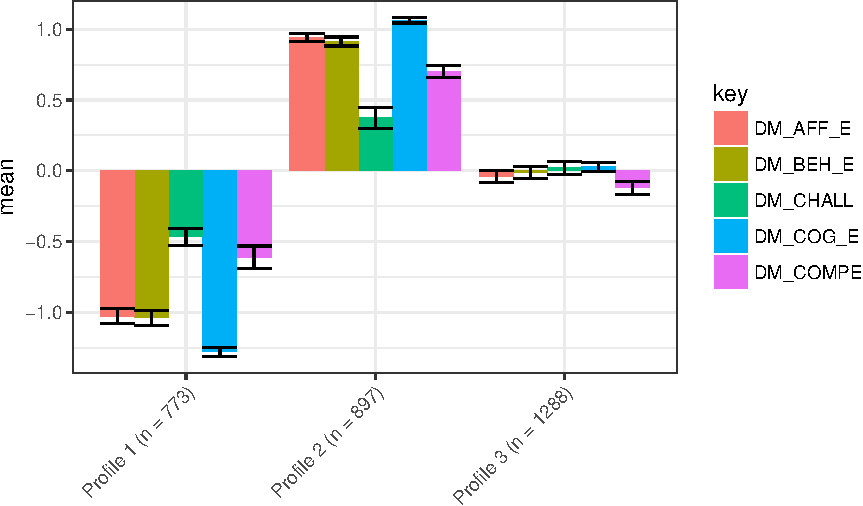
\includegraphics[width=0.8\linewidth]{rosenberg-dissertation_files/figure-latex/m1_3p-1} \end{center}

\subsubsection{Model: 1, Profiles: 4}\label{model-1-profiles-4}

This solution is characterized by:

\begin{itemize}
\tightlist
\item
  a \textbf{full} profile, profile 2
\item
  a \textbf{universally low} profile, profile 1
\item
  an \textbf{all moderate} profile, profile 3.
\item
  a \textbf{competent but not engaged or challenged} profile, with high
  levels of competence and low levels of engagement and challenge
\end{itemize}

Most profiles are in the all moderate profile (\emph{n} = 1,288), with a
large number in the full (\emph{n} = 920) profile, and fewer in the
universally low and competent (\emph{n} n = 427) but not engaged or
challenged profiles (\emph{n} = 415). With somewhat more purchase in
terms of its interpretability than the solution for model 1 with three
profiles, like that solution, this one may not be as useful as more
complex models for understanding youth's experiences.

The log-likelihood was replicated many (more than 10) times.

\begin{center}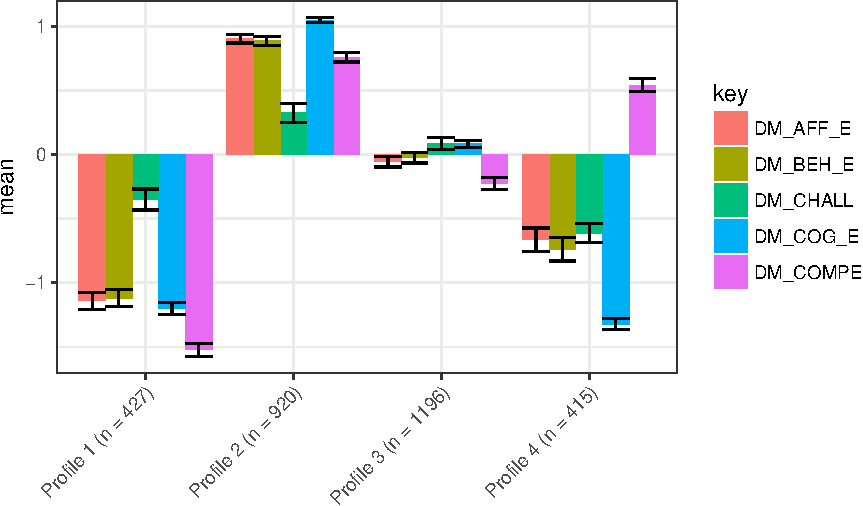
\includegraphics[width=0.8\linewidth]{rosenberg-dissertation_files/figure-latex/m1_4p-1} \end{center}

\subsubsection{Model: 1, Profiles: 5}\label{model-1-profiles-5}

This solution is characterized by:

\begin{itemize}
\tightlist
\item
  a \textbf{full} profile, profile 5
\item
  a \textbf{universally low} profile, profile 3
\item
  an \textbf{all moderate} profile, profile 3, though with moderate
  levels of affective engagement than in similar profiles associated
  with the four and five profile solutions, perhaps suggesting that a
  different profile than in those solutions
\item
  an \textbf{only behavioral} profile, profile 2, with moderate levels
  of behavioral engagement, very low affective engagement, and
  moderately (low) levels of cognitive engagement and challenge and
  competence
\item
  an \textbf{only affective} profile, profile 4, with moderate levels of
  affective engagement, low levels of behavioral engagement, and
  moderately (low) levels of cognitive engagement and challenge and
  competence
\end{itemize}

The number of observations associated with each of the profiles is
somewhat balanced, with a large number in the full profile (\emph{n} =
928), a moderate number of observations in the universally low (\emph{n}
= 667) and all moderate (\emph{n} = 643) profiles, and fewer
observations in the only behaviorally engaged (\emph{n} = 375) and only
affective engaged (\emph{n} = 345) profiles. This solution primarily
distinguishes between affective and behavioral engagement; unlike the
solution for model 1 with four profiles, there is not a competent but
not engaged or challenged profile. This may suggest that solutions with
a greater number of profiles represents both the distinction between
behavioral and affective engagement highlighted by profiles in this
solution as well as profiles that are characterized by higher or lower
levels of the conditions for engagement (i.e., competence). The
log-likelihood was replicated four times.

\begin{center}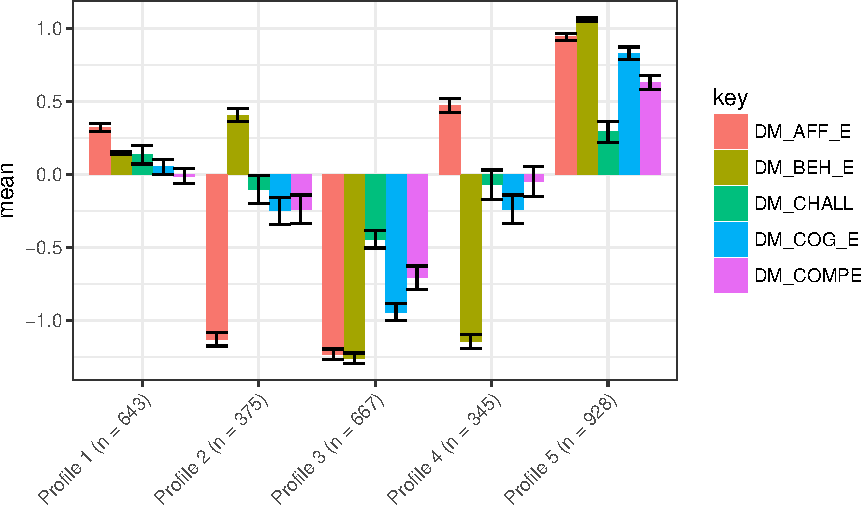
\includegraphics[width=0.8\linewidth]{rosenberg-dissertation_files/figure-latex/m1_5p-1} \end{center}

\subsubsection{Model: 1, Profiles: 6
(alternate)}\label{model-1-profiles-6-alternate}

This solution is characterized by:

\begin{itemize}
\tightlist
\item
  a \textbf{full} profile, profile 6
\item
  a \textbf{universally low} profile, profile 1
\item
  an \textbf{engaged and competent but not challenged} profile, profile
  3
\item
  a \textbf{challenged} profile, profile 2
\item
  a \textbf{highly challenged} profile, profile 3
\item
  a \textbf{moderately low} profile, profile 5
\end{itemize}

The number of observations are not very balanced, with the moderately
low profile with a large number of observations (\emph{n} = 852) and the
challenged, engaged and competent but not challenged, and full profiles
with moderate numbers of observations (from 464 to 619 observations),
and low numbers of observations exhibited by universally low (\emph{n} =
280) and highly challenged (\emph{n} = 158) profiles. This--and,
critically, the lower log-likelihood of the other model 1, six profile
solution--suggests that this solution is not preferred. However, the
very different profiles that emerge for this solution suggest that there
might not be a somewhat under-identified solution associated with model
1 and six profiles.

\begin{center}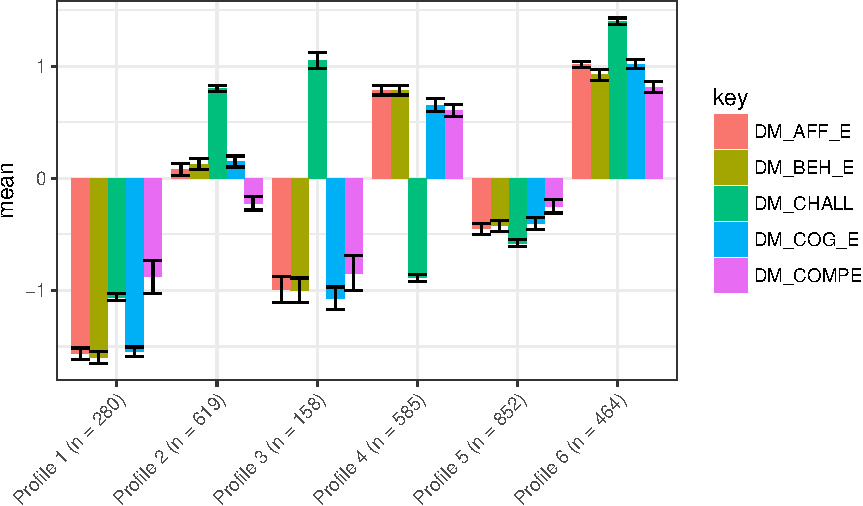
\includegraphics[width=0.8\linewidth]{rosenberg-dissertation_files/figure-latex/m1_6p-alt-1} \end{center}

\subsubsection{Model: 1, Profiles: 7
(alternate)}\label{model-1-profiles-7-alternate}

When investigating an alternate solution (associated with the second
lowest log-likelihood) for the model 1, seven profile solution, we can
see that even for the solutions associated with other log-likelihoods,
the profiles that can be identified are very similar. One minor
distinction concerns the \textbf{competent but not engaged or
challenged} profile, which in the alternate solution is associated with
neutral levels of affective engagement, compared to moderately low
levels of affective engagement in the solution with the lowest
log-likelihood. Because five of the seven profiles associated with both
of these model 1, seven profile solutions seem to be distinct from those
identified from simpler model 1 solutions, investigation of this
alternate solution provides additional evidence that these profiles are
not associated with an under-identified model and that simpler models
may be preferred over these seven profile solutions.

\begin{center}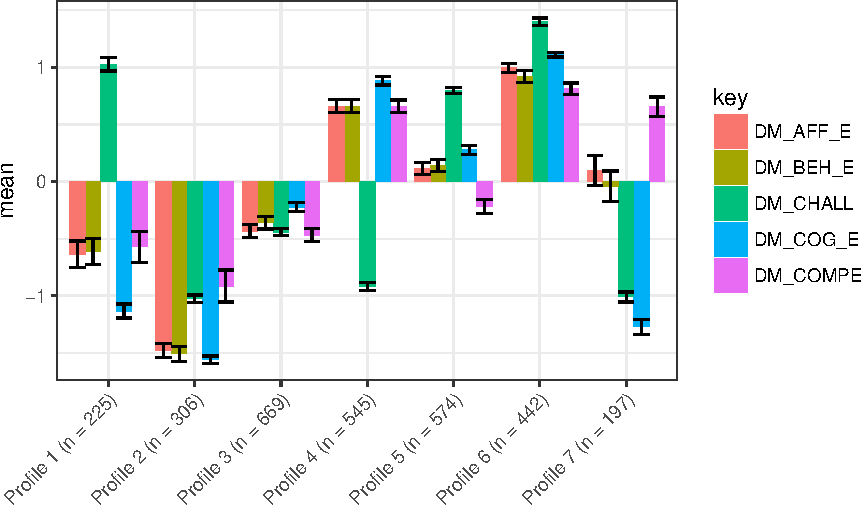
\includegraphics[width=0.8\linewidth]{rosenberg-dissertation_files/figure-latex/m1_7-other-LL-p-1} \end{center}

\subsection{Model 2 candidate
solutions}\label{model-2-candidate-solutions}

\subsubsection{Model: 2, Profiles: 3}\label{model-2-profiles-3}

This solution is characterized by:

\begin{itemize}
\tightlist
\item
  a \textbf{universally low} profile, profile 1, associated with
  moderate (low) and low levels of all of the variables; this profile is
  similar to the universally low profile identified as part of other
  solutions, although with more moderate values for some of the
  variables (especially cognitive engagement)
\item
  a \textbf{competent but not challenged} profile, profile 2,
  characterized by high competence and low challenge
\item
  a \textbf{challenged} profile, profile 3, characterized by very high
  challenge and moderate (high) levels of the other variables, similar
  to the challenged profile found as part of the model 1, four profile
  solution, but with higher levels of competence, which are moderately
  high in this solution but moderately low for the other solution.
\end{itemize}

The number of observations associated with each solution is fairly
balanced, with the most in the challenged profile (\emph{n} = 1,241),
followed by the universally low (\emph{n} = 954 observations) and
competent but not challenged (\emph{n} = 763) profiles. This solution is
very different than the three profile solution that was interpreted for
model 1. Model 2 differs from model 1 in that covariances between the
variables are estimated (they are constrained to be the same are across
the profiles). The log-likelihood was replicated (at least) ten times.
Thus, this and other solutions associated with model 2 include
information about how the variables relate. Including this information
seems to be associated with profiles that differentiate the groups on
the basis of the levels of each of the variables in more distinct ways:
the model 1, three profile solution was characterized by high, moderate,
or low levels of all variables for each of the three profiles.

\begin{center}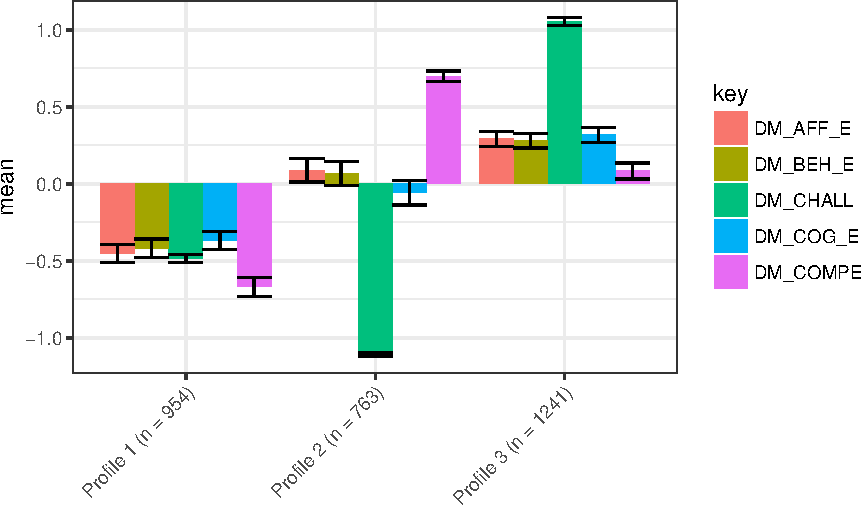
\includegraphics[width=0.8\linewidth]{rosenberg-dissertation_files/figure-latex/m2_3p-1} \end{center}

\subsubsection{Model: 2, Profiles: 4}\label{model-2-profiles-4}

This solution is characterized by:

\begin{itemize}
\tightlist
\item
  a \textbf{universally low} profile, profile 1
\item
  a \textbf{challenged} profile, profile 2
\item
  a \textbf{highly challenged} profile, profile 4
\item
  an \textbf{engaged and competent but not challenged} profile, profile
  3
\end{itemize}

The number of observations in each of the profiles is not very balanced,
with more than 1,000 observations in both the universally low (\emph{n}
= 1,029) and challenged (\emph{n} = 1,106) profiles, a moderate number
if the engaged and competent but not challenged profile (\emph{n} =
688), and very few in the highly challenged (\emph{n} = 135) profile.
The log-likelihood was replicated three times. While each of these
profiles has been identified in another solution, the small number of
observations in the highly challenged profile suggests that this
solution be interpreted with some skepticism because of the potentially
limited utility (and statistical power associated with the use) of the
profiles in subsequent analyses.

\begin{center}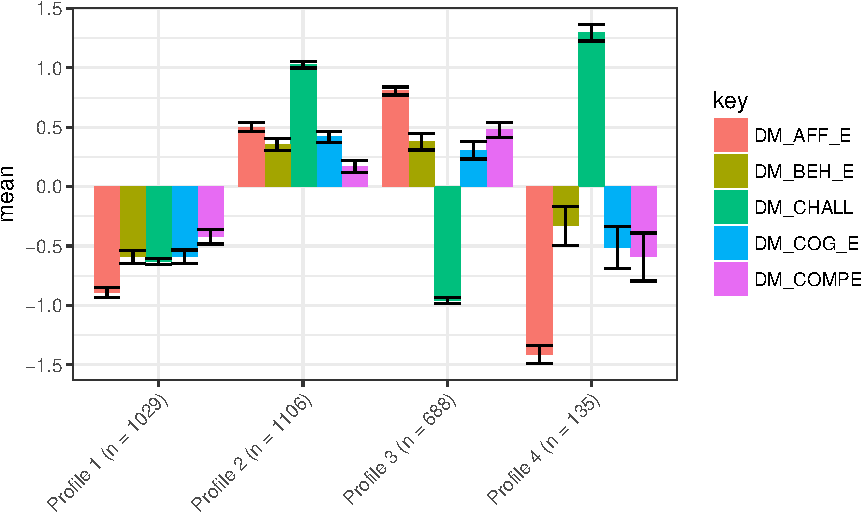
\includegraphics[width=0.8\linewidth]{rosenberg-dissertation_files/figure-latex/m2_4p-1} \end{center}

\subsubsection{Model: 2, Profiles: 5}\label{model-2-profiles-5}

This solution is characterized by:

\begin{itemize}
\tightlist
\item
  a \textbf{universally low} profile, profile 1
\item
  a \textbf{full} profile, profile 4, although with very high levels of
  challenged (in addition to high levels of all of the other variables),
  making this profile similar to that (challenged) profile
\item
  a \textbf{highly challenged} profile, profile 5
\item
  an \textbf{all moderate} profile, profile 3, although with moderately
  lower levels of competence than is found in profiles associated with
  other solutions
\item
  a \textbf{competent but not challenged} profile, profile 2, similar to
  the competent but not challenged or engaged profile, but with neutral,
  rather than low, levels of the engagement variables
\end{itemize}

The number of observations associated with each of the profiles is not
very balanced, with a very large number of observations in the all
moderate profile (\emph{n} = 1,113) and a large number in the competent
but not challenged profile (\emph{n} = 871), a moderate number in the
full profile (\emph{n} = 573), and very few in the universally low
(\emph{n} = 271) and challenged but not competent (\emph{n} = 130)
profiles. The log-likelihood was replicated four times. Like for the
model 2, four profile solution, the small number of observations
associated with two of the profiles suggests that this solution should
be interpreted with some caution.

\begin{center}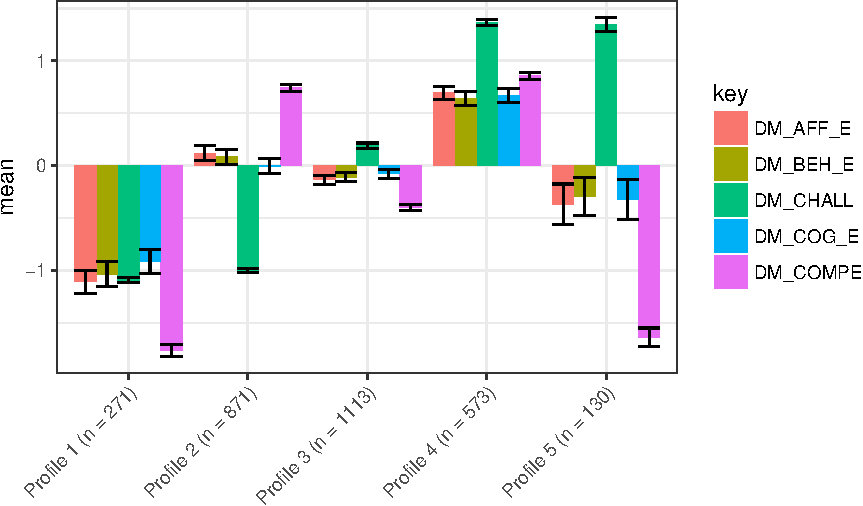
\includegraphics[width=0.8\linewidth]{rosenberg-dissertation_files/figure-latex/m2_5p-1} \end{center}

\section{Appendix: Models for research question \#2 and \#3 with the
seven-profile
solution}\label{appendix-models-for-research-question-2-and-3-with-the-seven-profile-solution}

\begin{landscape}\begin{table}

\caption{\label{tab:rq2-1-tab-pres-i}Results of mixed effects models for instructional support for work with data as separate variables}
\centering
\resizebox{\linewidth}{!}{\begin{tabular}[t]{lllllllrrr}
\toprule
model & intercept & dm\_ask & dm\_obs & dm\_gen & dm\_mod & dm\_com & beep\_ID\_ICC & participant\_ID\_ICC & program\_ID\_ICC\\
\midrule
Universally low & 0.072 (0.01) (p < .001) & -0.011 (0.011) (p = 0.839) & 0.001 (0.011) (p = 0.457) & -0.005 (0.01) (p = 0.686) & -0.002 (0.011) (p = 0.58) & -0.002 (0.01) (p = 0.583) & 0.008 & 0.176 & 0.002\\
Competent but not engaged or challenged & 0.111 (0.019) (p < .001) & 0.002 (0.013) (p = 0.428) & -0.007 (0.013) (p = 0.696) & -0.01 (0.012) (p = 0.78) & -0.025 (0.014) (p = 0.969) & -0.002 (0.013) (p = 0.549) & 0.014 & 0.222 & 0.021\\
Moderately low & 0.186 (0.029) (p < .001) & 0.024 (0.017) (p = 0.077) & 0.024 (0.017) (p = 0.074) & 0.009 (0.016) (p = 0.281) & -0.002 (0.018) (p = 0.544) & 0.027 (0.017) (p = 0.053) & 0.016 & 0.279 & 0.033\\
Challenged & 0.197 (0.023) (p < .001) & 0.011 (0.016) (p = 0.252) & -0.013 (0.016) (p = 0.799) & 0.034 (0.015) (p = 0.015) & -0.005 (0.017) (p = 0.626) & -0.002 (0.016) (p = 0.561) & 0.007 & 0.261 & 0.015\\
Highly challenged & 0.083 (0.01) (p < .001) & -0.007 (0.012) (p = 0.714) & 0 (0.012) (p = 0.504) & -0.016 (0.012) (p = 0.913) & 0.017 (0.013) (p = 0.1) & -0.013 (0.012) (p = 0.859) & 0.023 & 0.104 & 0.000\\
Engaged and competent but not challenged & 0.199 (0.018) (p < .001) & -0.014 (0.017) (p = 0.787) & 0.019 (0.017) (p = 0.129) & -0.033 (0.016) (p = 0.979) & -0.013 (0.018) (p = 0.77) & 0.019 (0.017) (p = 0.127) & 0.015 & 0.286 & 0.000\\
Full & 0.154 (0.023) (p < .001) & -0.009 (0.014) (p = 0.748) & -0.024 (0.014) (p = 0.961) & 0.022 (0.013) (p = 0.048) & 0.032 (0.014) (p = 0.012) & -0.025 (0.013) (p = 0.97) & 0.018 & 0.513 & 0.012\\
\bottomrule
\end{tabular}}
\end{table}
\end{landscape}

\begin{landscape}\begin{table}

\caption{\label{tab:just-composite-red-i}Results of mixed effects models for the composite}
\centering
\resizebox{\linewidth}{!}{\begin{tabular}[t]{lllrrr}
\toprule
model & intercept & dm\_composite & beep\_ID\_ICC & participant\_ID\_ICC & program\_ID\_ICC\\
\midrule
Universally low & 0.071 (0.01) (p < .001) & -0.004 (0.003) (p = 0.937) & 0.007 & 0.176 & 0.002\\
Competent but not engaged or challenged & 0.113 (0.019) (p < .001) & -0.008 (0.003) (p = 0.993) & 0.013 & 0.222 & 0.022\\
Moderately low & 0.188 (0.029) (p < .001) & 0.016 (0.004) (p < .001) & 0.015 & 0.279 & 0.032\\
Challenged & 0.2 (0.023) (p < .001) & 0.005 (0.004) (p = 0.09) & 0.007 & 0.260 & 0.015\\
Highly challenged & 0.08 (0.01) (p < .001) & -0.004 (0.003) (p = 0.917) & 0.022 & 0.104 & 0.000\\
Engaged and competent but not challenged & 0.2 (0.018) (p < .001) & -0.005 (0.004) (p = 0.887) & 0.015 & 0.285 & 0.000\\
Full & 0.151 (0.023) (p < .001) & 0 (0.003) (p = 0.527) & 0.019 & 0.510 & 0.013\\
\bottomrule
\end{tabular}}
\end{table}
\end{landscape}

\begin{landscape}\begin{table}

\caption{\label{tab:just-composite-red-2-i}Results of mixed effects models for the composite}
\centering
\resizebox{\linewidth}{!}{\begin{tabular}[t]{lllrrr}
\toprule
model & intercept & dm\_composite\_di & beep\_ID\_ICC & participant\_ID\_ICC & program\_ID\_ICC\\
\midrule
Universally low & 0.078 (0.012) (p < .001) & -0.02 (0.01) (p = 0.98) & 0.006 & 0.176 & 0.003\\
Competent but not engaged or challenged & 0.118 (0.019) (p < .001) & -0.03 (0.012) (p = 0.993) & 0.014 & 0.223 & 0.021\\
Moderately low & 0.175 (0.029) (p < .001) & 0.063 (0.016) (p < .001) & 0.015 & 0.279 & 0.031\\
Challenged & 0.203 (0.024) (p < .001) & 0.01 (0.015) (p = 0.261) & 0.008 & 0.260 & 0.014\\
Highly challenged & 0.083 (0.011) (p < .001) & -0.016 (0.011) (p = 0.922) & 0.023 & 0.104 & 0.000\\
Engaged and competent but not challenged & 0.198 (0.019) (p < .001) & -0.011 (0.016) (p = 0.763) & 0.015 & 0.285 & 0.000\\
Full & 0.146 (0.024) (p < .001) & 0.006 (0.013) (p = 0.308) & 0.019 & 0.510 & 0.014\\
\bottomrule
\end{tabular}}
\end{table}
\end{landscape}

\begin{landscape}\begin{table}

\caption{\label{tab:reading-for-rq4-i}Results of mixed effects models with interest and other characteristics}
\centering
\resizebox{\linewidth}{!}{\begin{tabular}[t]{lllllrrr}
\toprule
model & intercept & overall\_pre\_interest & gender\_female & urm & beep\_ID\_ICC & participant\_ID\_ICC & program\_ID\_ICC\\
\midrule
Universally low & 0.069 (0.04) (p = 0.042) & -0.002 (0.01) (p = 0.569) & 0.017 (0.018) (p = 0.177) & -0.005 (0.025) (p = 0.576) & 0.016 & 0.194 & 0.000\\
Competent but not engaged or challenged & 0.126 (0.049) (p = 0.006) & -0.011 (0.013) (p = 0.808) & 0.021 (0.022) (p = 0.165) & -0.007 (0.031) (p = 0.591) & 0.017 & 0.211 & 0.003\\
Moderately low & 0.301 (0.082) (p < .001) & -0.023 (0.021) (p = 0.869) & 0.02 (0.034) (p = 0.275) & -0.018 (0.048) (p = 0.642) & 0.017 & 0.290 & 0.030\\
Challenged & 0.297 (0.073) (p < .001) & -0.013 (0.019) (p = 0.757) & -0.04 (0.031) (p = 0.9) & -0.032 (0.044) (p = 0.768) & 0.013 & 0.254 & 0.016\\
Highly challenged & 0.108 (0.034) (p = 0.001) & -0.014 (0.009) (p = 0.946) & -0.013 (0.015) (p = 0.803) & 0.016 (0.021) (p = 0.221) & 0.026 & 0.112 & 0.001\\
Engaged and competent but not challenged & 0.065 (0.07) (p = 0.177) & 0.033 (0.018) (p = 0.034) & 0.042 (0.032) (p = 0.094) & -0.002 (0.045) (p = 0.518) & 0.013 & 0.275 & 0.000\\
Full & 0.048 (0.082) (p = 0.28) & 0.022 (0.021) (p = 0.142) & -0.043 (0.037) (p = 0.878) & 0.06 (0.053) (p = 0.129) & 0.023 & 0.510 & 0.000\\
\bottomrule
\end{tabular}}
\end{table}
\end{landscape}

\begin{landscape}\begin{table}

\caption{\label{tab:pre-int-ind-present-i}Results of mixed effects models with interest and other characteristics and the aspects of work with data}
\centering
\resizebox{\linewidth}{!}{\begin{tabular}[t]{llllllllllrrr}
\toprule
model & intercept & dm\_ask & dm\_obs & dm\_gen & dm\_mod & dm\_com & overall\_pre\_interest & gender\_female & urm & beep\_ID\_ICC & participant\_ID\_ICC & program\_ID\_ICC\\
\midrule
Universally low & 0.077 (0.041) (p = 0.031) & -0.01 (0.011) (p = 0.822) & 0.002 (0.011) (p = 0.429) & -0.003 (0.011) (p = 0.612) & -0.003 (0.012) (p = 0.616) & -0.002 (0.011) (p = 0.569) & -0.003 (0.01) (p = 0.63) & 0.017 (0.018) (p = 0.166) & -0.002 (0.025) (p = 0.535) & 0.008 & 0.189 & 0.004\\
Competent but not engaged or challenged & 0.141 (0.05) (p = 0.003) & 0.002 (0.013) (p = 0.432) & -0.011 (0.013) (p = 0.803) & -0.007 (0.013) (p = 0.718) & -0.028 (0.014) (p = 0.978) & 0.003 (0.013) (p = 0.421) & -0.013 (0.013) (p = 0.839) & 0.021 (0.022) (p = 0.167) & -0.011 (0.03) (p = 0.644) & 0.013 & 0.201 & 0.011\\
Moderately low & 0.271 (0.084) (p < .001) & 0.024 (0.018) (p = 0.087) & 0.027 (0.017) (p = 0.061) & 0.002 (0.017) (p = 0.447) & 0 (0.018) (p = 0.499) & 0.033 (0.017) (p = 0.03) & -0.024 (0.021) (p = 0.869) & 0.02 (0.034) (p = 0.284) & -0.019 (0.049) (p = 0.649) & 0.014 & 0.288 & 0.036\\
Challenged & 0.279 (0.075) (p < .001) & 0.018 (0.017) (p = 0.138) & -0.003 (0.017) (p = 0.568) & 0.029 (0.016) (p = 0.036) & -0.005 (0.017) (p = 0.606) & -0.006 (0.017) (p = 0.648) & -0.011 (0.019) (p = 0.725) & -0.042 (0.032) (p = 0.906) & -0.032 (0.045) (p = 0.762) & 0.007 & 0.253 & 0.022\\
Highly challenged & 0.128 (0.035) (p < .001) & -0.004 (0.013) (p = 0.63) & -0.008 (0.013) (p = 0.722) & -0.016 (0.012) (p = 0.9) & 0.023 (0.014) (p = 0.048) & -0.022 (0.013) (p = 0.951) & -0.015 (0.009) (p = 0.959) & -0.009 (0.015) (p = 0.721) & 0.013 (0.021) (p = 0.263) & 0.025 & 0.108 & 0.000\\
Engaged and competent but not challenged & 0.071 (0.071) (p = 0.161) & -0.018 (0.017) (p = 0.854) & 0.017 (0.017) (p = 0.164) & -0.027 (0.016) (p = 0.948) & -0.013 (0.018) (p = 0.759) & 0.017 (0.017) (p = 0.168) & 0.034 (0.018) (p = 0.034) & 0.046 (0.032) (p = 0.079) & -0.001 (0.045) (p = 0.509) & 0.013 & 0.279 & 0.000\\
Full & 0.053 (0.085) (p = 0.266) & -0.015 (0.014) (p = 0.852) & -0.026 (0.014) (p = 0.967) & 0.022 (0.013) (p = 0.048) & 0.029 (0.015) (p = 0.026) & -0.022 (0.014) (p = 0.938) & 0.023 (0.021) (p = 0.148) & -0.043 (0.038) (p = 0.868) & 0.063 (0.055) (p = 0.127) & 0.021 & 0.534 & 0.000\\
\bottomrule
\end{tabular}}
\end{table}
\end{landscape}

\begin{landscape}\begin{table}

\caption{\label{tab:pre-int-int-present-i}Results of mixed effects models with interest and other characteristics and the composite work with data}
\centering
\resizebox{\linewidth}{!}{\begin{tabular}[t]{llllllrrr}
\toprule
model & intercept & dm\_composite & overall\_pre\_interest & gender\_female & urm & beep\_ID\_ICC & participant\_ID\_ICC & program\_ID\_ICC\\
\midrule
Universally low & 0.077 (0.041) (p = 0.031) & -0.004 (0.003) (p = 0.908) & -0.004 (0.01) (p = 0.632) & 0.017 (0.018) (p = 0.168) & -0.002 (0.025) (p = 0.533) & 0.007 & 0.189 & 0.004\\
Competent but not engaged or challenged & 0.144 (0.05) (p = 0.002) & -0.008 (0.003) (p = 0.992) & -0.013 (0.013) (p = 0.841) & 0.022 (0.022) (p = 0.159) & -0.012 (0.03) (p = 0.65) & 0.012 & 0.201 & 0.012\\
Moderately low & 0.273 (0.083) (p < .001) & 0.017 (0.004) (p < .001) & -0.024 (0.021) (p = 0.871) & 0.02 (0.034) (p = 0.278) & -0.019 (0.049) (p = 0.653) & 0.013 & 0.288 & 0.034\\
Challenged & 0.28 (0.075) (p < .001) & 0.007 (0.004) (p = 0.044) & -0.011 (0.019) (p = 0.717) & -0.042 (0.032) (p = 0.905) & -0.032 (0.045) (p = 0.763) & 0.006 & 0.253 & 0.022\\
Highly challenged & 0.125 (0.035) (p < .001) & -0.005 (0.003) (p = 0.951) & -0.016 (0.009) (p = 0.964) & -0.01 (0.015) (p = 0.733) & 0.014 (0.021) (p = 0.254) & 0.024 & 0.109 & 0.000\\
Engaged and competent but not challenged & 0.072 (0.071) (p = 0.156) & -0.006 (0.004) (p = 0.911) & 0.033 (0.018) (p = 0.035) & 0.046 (0.032) (p = 0.078) & 0 (0.045) (p = 0.503) & 0.012 & 0.279 & 0.000\\
Full & 0.05 (0.085) (p = 0.278) & -0.001 (0.004) (p = 0.657) & 0.023 (0.021) (p = 0.143) & -0.045 (0.038) (p = 0.878) & 0.063 (0.055) (p = 0.126) & 0.022 & 0.532 & 0.000\\
\bottomrule
\end{tabular}}
\end{table}
\end{landscape}

\begin{landscape}\begin{table}

\caption{\label{tab:pre-int-comp-i}Results of mixed effects models with the interactions between interest and other characactistics and the composite for work with data}
\centering
\resizebox{\linewidth}{!}{\begin{tabular}[t]{lllllllllrrr}
\toprule
model & intercept & dm\_composite & overall\_pre\_interest & gender\_female & urm & overall\_pre\_interest:dm\_composite & dm\_composite:gender\_female & dm\_composite:urm & beep\_ID\_ICC & participant\_ID\_ICC & program\_ID\_ICC\\
\midrule
Universally low & 0.113 (0.046) (p = 0.008) & -0.022 (0.012) (p = 0.973) & -0.014 (0.012) (p = 0.878) & 0.025 (0.021) (p = 0.113) & -0.012 (0.029) (p = 0.663) & 0.005 (0.003) (p = 0.038) & -0.004 (0.005) (p = 0.761) & 0.005 (0.007) (p = 0.225) & 0.007 & 0.189 & 0.004\\
Competent but not engaged or challenged & 0.133 (0.056) (p = 0.009) & -0.002 (0.013) (p = 0.553) & -0.01 (0.015) (p = 0.761) & 0.031 (0.025) (p = 0.106) & -0.013 (0.035) (p = 0.643) & -0.001 (0.003) (p = 0.656) & -0.005 (0.006) (p = 0.784) & 0.001 (0.008) (p = 0.466) & 0.012 & 0.201 & 0.011\\
Moderately low & 0.256 (0.089) (p = 0.002) & 0.026 (0.017) (p = 0.071) & -0.017 (0.023) (p = 0.774) & 0.015 (0.038) (p = 0.345) & -0.02 (0.053) (p = 0.643) & -0.003 (0.005) (p = 0.767) & 0.003 (0.008) (p = 0.376) & 0 (0.011) (p = 0.505) & 0.013 & 0.287 & 0.034\\
Challenged & 0.262 (0.082) (p < .001) & 0.016 (0.017) (p = 0.178) & -0.002 (0.021) (p = 0.542) & -0.063 (0.035) (p = 0.961) & -0.03 (0.05) (p = 0.724) & -0.004 (0.005) (p = 0.83) & 0.011 (0.008) (p = 0.094) & -0.002 (0.011) (p = 0.573) & 0.006 & 0.253 & 0.022\\
Highly challenged & 0.12 (0.042) (p = 0.002) & -0.003 (0.013) (p = 0.608) & -0.018 (0.011) (p = 0.951) & -0.015 (0.019) (p = 0.778) & 0.03 (0.026) (p = 0.126) & 0.001 (0.003) (p = 0.368) & 0.003 (0.006) (p = 0.317) & -0.008 (0.008) (p = 0.851) & 0.025 & 0.108 & 0.000\\
Engaged and competent but not challenged & 0.07 (0.078) (p = 0.185) & -0.004 (0.017) (p = 0.593) & 0.029 (0.02) (p = 0.079) & 0.065 (0.036) (p = 0.034) & 0.007 (0.05) (p = 0.441) & 0.002 (0.005) (p = 0.319) & -0.01 (0.008) (p = 0.888) & -0.003 (0.011) (p = 0.624) & 0.012 & 0.277 & 0.000\\
Full & 0.073 (0.088) (p = 0.205) & -0.014 (0.013) (p = 0.848) & 0.021 (0.022) (p = 0.172) & -0.057 (0.04) (p = 0.921) & 0.049 (0.057) (p = 0.196) & 0.001 (0.003) (p = 0.38) & 0.006 (0.006) (p = 0.148) & 0.007 (0.008) (p = 0.202) & 0.022 & 0.532 & 0.000\\
\bottomrule
\end{tabular}}
\end{table}
\end{landscape}

\bibliography{book.bib,packages.bib}


\end{document}
